\documentclass[utf8,german,fpg,lot,lof,lol]{zihpub}

\usepackage{algorithmicx}
\usepackage{algpseudocode}
\usepackage{caption}
\usepackage{chngcntr} % Bilder pro section zählen
\usepackage{datetime}
\usepackage{etoolbox}
\usepackage{float}
\usepackage[acronyms,nonumberlist,nopostdot,toc,savewrites,xindy]{glossaries}
\usepackage[section,newfloat]{minted}
\usepackage[super]{nth}
\usepackage{pgfplots}
\usepackage[binary-units]{siunitx}
\usepackage{subcaption}
\usepackage{textcomp}
\usepackage{tcolorbox}
\usepackage{tikz}
\usepackage{tkz-berge}
\usepackage{xintexpr} % weil PGFPlots zu dämlich für 1024 ist

% Bilder pro section
\counterwithin{figure}{section}

\usetikzlibrary{arrows}
\usetikzlibrary{arrows.meta}

\pgfplotsset{
    /pgfplots/peak/.style = {
        legend image code/.code = {
            \draw[solid,thick,red](-0.05cm,0cm) -- (0.3cm, 0cm);
        }
    }
}

\usepackage{CJKutf8}
\AtBeginDvi{\input{zhwinfonts}}

\makeglossaries

\newacronym{api}{API}{\textit{application programming interface}}
\newacronym{apu}{APU}{\textit{accelerated processing unit}}

\newacronym{cpu}{CPU}{\textit{central processing unit}}

\newacronym{dsp}{DSP}{\textit{digital signal processor}}

\newacronym{fpga}{FPGA}{\textit{field programmable gate array}}

\newacronym{gpgpu}{GPGPU}{\textit{general purpose computation on graphics processing unit}}
\newacronym{gpu}{GPU}{\textit{graphics processing unit}}

\newacronym{hc}{HC}{\textit{Heterogeneous Compute API}}
\newacronym{hcc}{HCC}{\textit{Heterogeneous Compute Compiler}}
\newacronym{hip}{HIP}{\textit{Heterogeneous-Computing Interface for Portability}}
\newacronym{hpc}{HPC}{\textit{high-performance computing}}
\newacronym{hsa}{HSA}{\textit{Heterogeneous System Architecture}}

\newacronym{numa}{NUMA}{\textit{non-uniform memory access}}

\newacronym{openacc}{OpenACC}{\textit{Open Accelerators}}
\newacronym{opencl}{OpenCL}{\textit{Open Compute Language}}
\newacronym{openmp}{OpenMP}{\textit{Open Multi-Processing}}

\newacronym{rock}{ROCk}{\textit{Radeon Open Compute Kernel driver}}
\newacronym{rocm}{ROCm}{\textit{Radeon Open Compute Platform}}
\newacronym{rocr}{ROCr}{\textit{Radeon Open Compute Platform Runtime}}
\newacronym{roct}{ROCt}{\textit{Radeon Open Compute Thunk Interface}}

\newglossaryentry{kernel}{name = Kernel,
                          description = {Programm, das auf einem Beschleuniger,
                                         wie etwa einer GPU, ausgeführt wird.},
                          plural = Kernel}
\newglossaryentry{host}{name = Host,
                        description = {Gerät, das einen Kernel auf dem Device
                                       ausführen lässt. Üblicherweise das Gerät,
                                       auf dem das Betriebssystem läuft, etwa
                                       ein PC oder ein Knoten auf einem
                                       Superrechner.},
                        plural = Hosts}
\newglossaryentry{device}{name = Device,
                          description = {Gerät, das einen Kernel ausführt. Im
                                         Kontext dieser Arbeit stets eine GPU.},
                          plural = Devices}
\newglossaryentry{singlesource}{name = {single-source compilation},
                                description = {Die Quelltexte für Host und
                                               Device werden gleichzeitig vom
                                               Compiler für die
                                               Zielarchitekturen übersetzt.}}
\newglossaryentry{splitsource}{name = {split-source compilation},
                               description = {Die Quelltexte für Host und
                                              Device werden getrennt kompiliert.
                                              Der Host-Quelltext wird von einem
                                              normalen Compiler übersetzt, der
                                              Device-Quelltext erst zur Laufzeit
                                              des Programms von einem weiteren
                                              Compiler.}}


\newenvironment{code}{\captionsetup{type=listing}}{}
\SetupFloatingEnvironment{listing}{name=Quelltext}

\BeforeBeginEnvironment{minted}{\begin{tcolorbox}}
\AfterEndEnvironment{minted}{\end{tcolorbox}}

\newcommand{\lstfont}[1]{\color{#1}\small\ttfamily}

\definecolor{keyword-green}{RGB}{0, 128, 0}

\author{Jan Stephan}
\title{Innovative Spracherweiterungen für Beschleunigerkarten am Beispiel von
       SYCL, HCC, HIP und CUDA: Untersuchung zu Nutzbarkeit und Performance}
\matno{3755136}
\betreuer{\hspace{0.15mm}Dr.-Ing.\ Bernd Trenkler\\
          \qquad \qquad Matthias Werner, M.Sc.}
\date{21.\ Februar 2019}

\bibfiles{bibliography.bib}
\def\UrlBreaks{\do\/\do-}

% Germanisiere LaTeX
\deftranslation[to=German]{Acronyms}{Abkürzungsverzeichnis}
\deftranslation[to=German]{Glossary}{Glossar}
\renewcommand*{\listlistingname}{Quelltextverzeichnis}

\sisetup{locale = DE}
\sisetup{group-separator = {.}}
\sisetup{group-four-digits}

\fancyhf{}
\fancyhead[L]{Jan Stephan -- Innovative Spracherweiterungen}

\begin{document}

\glsaddall

\printglossary
\printglossary[type=\acronymtype]

\section{Einleitung}
\label{einleitung}

\subsection{Motivation}
\label{einleitung:motivation}

Das Feld der \gls{gpgpu} ist seit 2006 vor allem durch NVIDIAs CUDA-Plattform
und GPUs geprägt und dominiert worden. Die Konkurrenz (vor allem der
GPU-Hersteller AMD) konnte dem lange Zeit wenig entgegensetzen -- heute
(November 2018) sind NVIDIA-GPUs in fünf der zehn leistungsstärksten
Supercomputer vorhanden, darunter die ersten beiden Plätze. Auf der Liste der
500 leistungsstärksten Supercomputer finden sich mit NVIDIA-GPUs bestückte
Rechner insgesamt 126 Mal, GPUs des größten Konkurrenten AMD kein einziges Mal.
Intels als GPU-Alternative vor- und mittlerweile zugunsten einer noch
unbekannten zukünftigen Plattform (vgl.~\cite{intel2017}) eingestellten
Xeon-Phi-Beschleuniger sind auf dieser Liste noch 30 Mal vertreten.
(vgl.~\cite{top500})

Softwareseitig entstand ab 2008 mit der von Apple entwickelten und vom
Khronos-Industriekonsortium standardisierten \gls{opencl} ein offener und
hardware-übergreifender Konkurrent der CUDA-Plattform, der zunächst von einer
Reihe wichtiger Hersteller (einschließlich NVIDIA) unterstützt wurde. Im 
Gegensatz zu CUDA wurde \gls{opencl} von Anfang an auf verschiedene Arten von
Beschleunigern ausgelegt, wie etwa Systeme mit einem \gls{dsp} oder einem
\gls{fpga}. Mit der Zeit zeigte sich jedoch, dass die Unterstützung durch die
Hersteller mit jeder weiteren Revision des Standards abnahm; so ist die 2011
erschienene \gls{opencl}-Version 1.2 bis heute die neueste Version, die von
NVIDIA und AMD\footnote{AMD unterstützte zwischenzeitlich \gls{opencl} 2.0, ist
jedoch infolge des Umbaus des eigenen Treiber- und Compute-Ökosystems auf
\gls{opencl} 1.2 zurückgegangen.} vollständig unterstützt wird. Lediglich Intel
bietet eine Implementierung eines modernen \gls{opencl}-Standards an, beschränkt
sich dabei aber auf seine CPUs und integrierten GPUs. Eine
\gls{opencl}-Implementierung für die neuesten Produktlinien der Xeon-Phi-Reihe,
\textit{Knights Landing} und \textit{Knights Mill}, existiert nicht, während
\gls{opencl} 1.0 (2008) die einzige verfügbare Version für \gls{fpga}s
darstellt.

Sowohl Khronos als auch AMD versuchen seit einigen Jahren, durch neue
Technologien im Umfeld des \gls{hpc} wieder Anschluss an NVIDIA zu finden. Im
März 2014 stellte Khronos den SYCL-Standard vor, der auf \gls{opencl}s Konzepten
und Portabilität aufbaut, jedoch eine auf C++ basierende, deutlich modernere
und angenehmere Programmierweise bieten soll. AMD folgte im April 2016 mit einer
eigenen, quelloffenen Plattform namens \gls{rocm}, die neben einer
Portabilitätsschicht zu CUDA (\gls{hip}) einen auf AMD-GPUs spezialisierten
C++-Dialekt (\gls{hc}) bietet.

Beide Ansätze befinden sich im Gegensatz zu CUDA noch am Anfang ihrer
Entwicklung und erfahren laufend größere Änderungen sowie Feature-Updates. Eine
vergleichende Untersuchung der bereits verfügbaren Fähigkeiten und Konzepte 
sowohl untereinander als auch im Vergleich zu CUDA ist jedoch möglich und in
der wissenschaftlichen Literatur bisher nicht aufzufinden.

\subsection{Forschungsstand}
\label{einleitung:forschung}

Die wissenschaftliche Literatur betrachtet SYCL vornehmlich als
Abstraktionsschicht über \gls{opencl}. Aus diesem Grund sind Untersuchungen, die
sich direkt auf SYCL fokussieren, relativ selten.

Das im März 2014 veröffentlichte SYCL wurde erstmals im August des selben Jahres
von Trigkas untersucht. Zu diesem Zweck wurde SYCL mit \gls{opencl} und
\gls{openmp} verglichen und auf Intels Xeon-Phi-Beschleunigern ausgeführt.
(vgl.~\cite{trigkas2014})

Cardoso da Silva et al.\ führten im Oktober 2016 ebenfalls einen Vergleich
zwischen SYCL, OpenCL und OpenMP durch, als Hardware kamen hier Intels Xeon-CPUs
zum Einsatz.
(vgl.~\cite{dasilva2016})

Jesenšek stellte 2017 eine SYCL-Implementierung für Intels
Xeon-Phi-Prozessoren und das Betriebssystem Linux vor.
(vgl.~\cite{jesensek2017})

Im Mai 2017 zeigten Goli et al.\, dass SYCL zur Beschleunigung des
Deep-Learning-Frameworks \textit{TensorFlow} eingesetzt werden kann.
(vgl.~\cite{goli2017})

Zur selben Zeit verwendeten Copik und Kaiser SYCL als Backend für das
\gls{hpc}-Programmiermodell \textit{HPX.Compute}.
(vgl.~\cite{copik2017})

Im selben Monat untersuchten Doumoulakis et al.\ die Interoperabilität zwischen
SYCL und \gls{opencl} auf GPUs und \gls{fpga}s.
(vgl.~\cite{doumoulakis2017})

Ebenfalls im selben Monat implementierten Aliaga et al.\ BLAS-Algorithmen auf
der Basis von Ausdrucksbäumen und SYCL.
(vgl.~\cite{aliaga2017})

St Clere Smithe und Potter stellten im Mai 2018 ein energieeffizientes
neuronales Netzwerk vor, das mittels SYCL implementiert wurde.
(vgl.~\cite{stcleresmithe2018})

Gleichzeitig zeigte Fare einen ersten Ansatz, der das Profiling von in SYCL
geschriebenen Anwendungen ermöglicht.
(vgl.~\cite{fare2018})

Zur selben Zeit präsentierten Keryell und Yu eine Untersuchung von
auf SYCL aufbauenden Programmen, die auf \gls{fpga}s ausgeführt werden.
(vgl.~\cite{keryell2018})

Afzal et al.\ lösten im Juli 2018 Maxwell-Gleichungen mit SYCL und verglichen
die Performance mit einer vorherigen Implementierung in der Programmiersprache
C.
(vgl.~\cite{afzal2018})

In der wissenschaftlichen Literatur tauchen die Begriffe \gls{rocm}, \gls{hc}
und \gls{hip} erstmals 2016 auf. Während sich die Arbeiten der ersten
Jahreshälfte vornehmlich mit der \gls{hsa} befassen und \gls{rocm} lediglich als
verwendeten Software-Unterbau erwähnen (vgl.\ etwa \cite{li2016},
\cite{larsson2016}), unternahm Sun im Juli 2016 den vermutlich ersten Vergleich
zwischen \gls{hip} und CUDA (vgl.~\cite{sun2016}. Es folgten viele verschiedene
Leistungsanalysen auf der Basis von \gls{rocm}:

Im September 2016 veröffentlichten Sun et al.\ ihre Benchmark-Suite
\textit{Hetero-Mark}, die vornehmlich die Leistungsfähigkeit von \gls{apu}s
misst und dabei auf \gls{rocm} und \gls{hc} aufsetzt (vgl.~\cite{sunyifan2016}).
Sun et al.\ nutzten \textit{Hetero-Mark} sowie das Framework \textit{DNNMark} im
April 2018 erneut, um \gls{rocm} einer eingehenden Performance-Analyse zu
unterziehen (vgl.~\cite{sun2018}). In die gleiche Richtung geht die im April
2017 von Gómez-Luna et al.\ vorgestellte Benchmark-Suite \textit{Chai}
(vgl.~\cite{gomezluna2017}). 

Im Mai 2017 stellten Hou et al.\ Benchmarks vor, die auf der Ebene der Register,
des L1-Caches und des \textit{shared memory} arbeiteten und in \gls{hc} und
CUDA implementiert wurden. (vgl.~\cite{hou2017})

Im Juli 2017 portierte Konstantinidis seine Sammlung von Micro-Benchmarks, die
die Leistungsfähigkeit von CUDA-\gls{gpu}s auf der Instruktionsebene prüfen,
mit der Hilfe von \gls{hip} auf die \gls{rocm}-Plattform.
(vgl.~\cite{konstantinidis2017})

Im Januar 2018 untersuchten Nobre et al.\ die Performanz und Genauigkeit von
Fließkommazahlen mit halber Präzision auf AMD \gls{gpu}s.
(vgl.~\cite{nobre2018})

\subsection{Zielstellung}
\label{einleitung:zielstellung}

Das Ziel dieser Arbeit ist ein vergleichende Analyse der Programmiermodelle
CUDA, SYCL und \gls{rocm} (bzw.\ \gls{hc} und \gls{hip}) auf GPUs der Hersteller
NVIDIA und AMD. Dabei sollen einerseits die den jeweiligen Modellen zugrunde
liegenden Fähigkeiten und Konzepte verglichen, andererseits die konkret
erreichbare Performanz anhand geeigneter Benchmarks ermittelt werden. Von den so
gewonnenen Erkenntnissen werden Empfehlungen für den zukünftigen Einsatz dieser
Modelle im \gls{hpc}-Umfeld abgeleitet.

\subsubsection{Anmerkung}

Die vollständigen Quelltexte und Ergebnisse der Benchmarks sowie die
\LaTeX-Quelltexte dieser Arbeit sind öffentlich unter dem folgenden Link
erreichbar: \url{https://github.com/j-stephan/fpg}

\section{Funktionaler Vergleich der Spracherweiterungen}
\label{vergleich}

\subsection{Anforderungen an Spracherweiterungen}
\label{vergleich:anforderungen}

Ein Vergleich der Fähigkeiten der einzelnen Spracherweiterungen erfordert einen
Kriterienkatalog, anhand dessen die Bewertung erfolgen kann. Dabei sind sowohl
die Sicht auf die Daten, also der Umgang der Spracherweiterungen mit den Daten,
als auch die Sicht auf die Aufgaben, also die Transformation der Daten, zu
berücksichtigen.

\subsubsection{Datensicht}
\label{vergleich:anforderungen:datensicht}

Der effiziente Umgang mit großen Datenmengen ist seit jeher eines der
Kernprobleme des \gls{hpc} im Allgemeinen und heterogener Systeme im Besonderen,
d.h.\ unterschiedlicher Berechnungs-Hardware im selben Rechnersystem. Michael
Wong\footnote{Mitglied des C++-Standard-Komitees, ehemaliger Projektleiter des
XL-C++-Compilers der Firma IBM und derzeit Entwicklungsleiter des Unternehmens
Codeplay, das unter anderem den SYCL-Standard implementiert} bezeichnete in
einem Vortrag im November 2018 vor LLVM-Entwicklern die folgenden Punkte als
essentielle Probleme der Programmierung heterogener Systeme
(vgl.~\cite{wong2018}):

\paragraph{Datenbewegung} 
Die Bewegung der Daten ist stets mit Kosten verbunden. Im Allgemeinen ist damit
der Zeitbedarf gemeint, um Daten etwa vom Hauptspeicher des Systems in den
Speicher der GPU zu kopieren. Im weiteren Sinne kann dieser Punkt aber auch
andere Kriterien umfassen, wie z.B.\ den für den Kopiervorgang notwendigen
Energiebedarf, der als Bestandteil des gesamten Energiebedarfs von
\gls{hpc}-Systemen in jüngerer Zeit ebenfalls Gegenstand der Forschung geworden
ist.

Aus der Sicht des Programmierers ist außerdem die Frage relevant, ob die
Datenbewegung \textit{explizit} oder \textit{implizit} erfolgt. Die
\textit{explizite} Datenbewegung hat den Vorteil, dass der Programmierer
jederzeit die volle Kontrolle über die Verschiebung und damit auch über die
Performanz hat, geht jedoch mit einer höheren Programmierkomplexität und damit
Fehleranfälligkeit einher. Überdies wird die volle Kontrolle nicht
notwendigerweise an jeder Stelle gebraucht und bläht damit den Quelltext unnötig
auf. Die Adressräume bleiben bei der expliziten Datenbewegung getrennt (siehe
Abbildung~\ref{vergleich:anforderungen:datensicht:explizitebewegung})

Diesem Ansatz steht die \textit{implizite} Datenbewegung gegenüber. Diese
überlässt den Zeitpunkt und den konkreten Vorgang des Kopierens oder
Verschiebens sowie den Umfang der bewegten Datenmenge der Laufzeitumgebung; aus
Sicht des Programmierers existiert ein virtueller Adressraum, den sich CPU und
GPU teilen (siehe
Abbildung~\ref{vergleich:anforderungen:datensicht:implizitebewegung}).

\begin{figure}[!hbt]
    \centering
    \begin{subfigure}{0.75\textwidth}
        \centering
        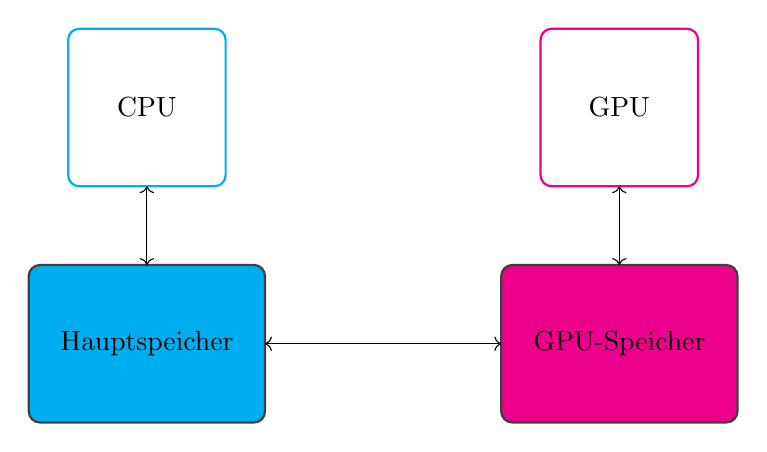
\begin{tikzpicture}
            \draw [thick, rounded corners, draw = cyan]
                  (-1.0, 0.0) rectangle (1.0, 2.0) node[pos = 0.5]
                  {CPU};

            \draw [thick, rounded corners, fill = cyan, draw = darkgray]
                  (-1.5, -3.0) rectangle (1.5, -1.0) node[pos = 0.5]
                  {Hauptspeicher};

            \draw [thick, rounded corners, draw = magenta]
                  (5.0, 0.0) rectangle (7.0, 2.0) node[pos=0.5] {GPU};

            \draw [thick, rounded corners, fill = magenta, draw = darkgray]
                  (4.5, -3.0) rectangle (7.5, -1.0) node[pos = 0.5]
                  {GPU-Speicher};

            \draw [<->] (0.0, 0.0) -- (0.0, -1.0); % CPU <-> RAM
            \draw [<->] (6.0, 0.0) -- (6.0, -1.0); % GPU <-> GPU-RAM
            \draw [<->] (1.5, -2.0) -- (4.5, -2.0); % RAM <-> GPU-RAM
        \end{tikzpicture}
        \caption{Sicht auf den Adressraum bei expliziter Datenbewegung.}
        \label{vergleich:anforderungen:datensicht:explizitebewegung}
    \end{subfigure}
    \par\bigskip
    \begin{subfigure}{0.75\textwidth}
        \centering
        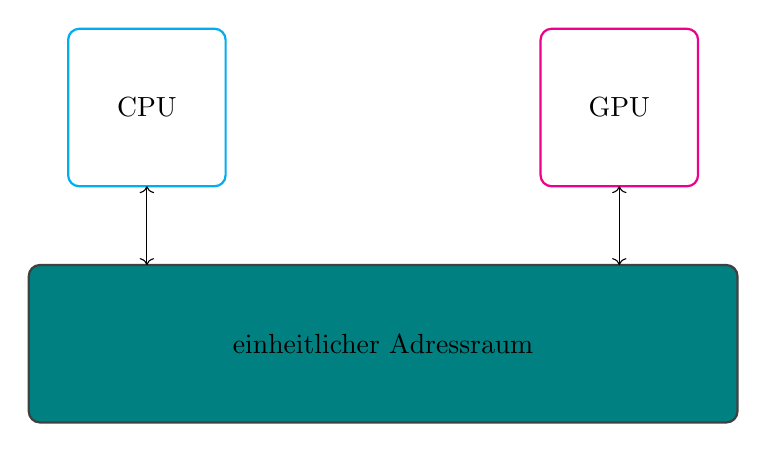
\begin{tikzpicture}
            \draw [thick, rounded corners, draw = cyan]
                  (-1.0, 0.0) rectangle (1.0, 2.0) node[pos = 0.5]
                  {CPU};

            \draw [thick, rounded corners, draw = magenta]
                  (5.0, 0.0) rectangle (7.0, 2.0) node[pos=0.5] {GPU};

            \draw [thick, rounded corners, fill = teal, draw = darkgray]
                  (-1.5, -3.0) rectangle (7.5, -1.0) node[pos = 0.5]
                  {einheitlicher Adressraum};

            \draw [<->] (0.0, 0.0) -- (0.0, -1.0); % CPU <-> Adressraum
            \draw [<->] (6.0, 0.0) -- (6.0, -1.0); % GPU <-> Adressraum
        \end{tikzpicture}
        \caption{Sicht auf den Adressraum bei impliziter Datenbewegung.}
        \label{vergleich:anforderungen:datensicht:implizitebewegung}
    \end{subfigure}
    \caption{Verschiedene Adressraumsichten}
    \label{vergleich:anforderungen:datensicht:adressraeume}
\end{figure}

Eine bewertende Gegenüberstellung beider Ansätze übersteigt den Rahmen dieser
Arbeit (und ist bisher auch in der Literatur nicht zu finden). Stattdessen wird
untersucht, in welcher Form beide Ansätze von den jeweiligen Spracherweiterungen
unterstützt werden.

\paragraph{Datenanordnung}

Die Anordnung der Daten im Speicher kann aufgrund einer Reihe von Faktoren, wie
etwa unterschiedlicher optimaler Zugriffsmuster von CPUs (\textit{cachelines})
und GPUs (\textit{strided access}), erheblich zur Performanz der Berechnung
beitragen. Aus Sicht des Programmieres ist es daher wünschenswert, dass die
Spracherweiterung eine abstrakte Sicht auf den von ihr verwendeten Speicher
bietet, welche die optimalen Zugriffsmuster der verschiedenen Hardware kapselt.

\paragraph{Datenaffinität}

Die Datenaffinität definiert die Zuordnung und Nähe eines Speicherbereichs zu
einer \textit{bestimmten} Ausführungseinheit, die auf diesen Speicherbereich
zugreifen muss. Im Hinblick auf GPUs meint dies die Zuordnung von im
Hauptspeicher liegenden Daten auf eine oder mehrere GPUs.

\paragraph{Datenlokalität}

Die obigen Punkte sind alle eng mit dem Aspekt der Datenlokalität verknüpft.
Im GPU-Kontext ist vornehmlich relevant, inwiefern sich die einzelnen
Ebenen der Speicherhierarchie (globaler Speicher der GPU, lokaler Speicher und
Cache der auf der GPU verbauten parallelen Prozessoren, Register der einzelnen
Threads) durch die Spracherweiterungen ansteuern und nutzen lassen.

\subsubsection{Aufgabensicht}
\label{vergleich:anforderungen:aufgabensicht}

Die im vorherigen Abschnitt genannten Punkte stellen die in dieser Arbeit
verwendeten Vergleichskriterien dar, bedürfen jedoch noch einer Ergänzung:

\paragraph{Aufgabengraphen}

Die Abfolge und Abhängigkeiten einzelner \textit{Kernel} lassen sich in Form
eines Graphen darstellen (siehe
Abbildung~\ref{vergleich:anforderungen:aufgabensicht:graph}). Eine effiziente
Ausnutzung der Parallelität voneinander unabhängiger Aufgaben setzt voraus,
dass Kernel \textit{asynchron} -- sowohl im Hinblick auf die CPU als auch
untereinander -- und \textit{parallel} auf der gleichen GPU ausgeführt werden
können. Im Rahmen dieser Arbeit wird deshalb ebenfalls untersucht, welche Mittel
die einzelnen Spracherweiterungen zur Verfügung stellen, um Aufgabengraphen zu
implementieren.

\begin{figure}[htb]
    \centering
    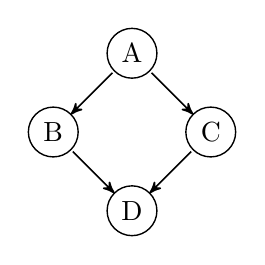
\begin{tikzpicture}
        \tikzstyle{every node} = [node distance = 3cm, fill = gray!30]

        \Vertex{B}
        \NOEA(B){A}
        \SOEA(B){D}
        \NOEA(D){C}

        \tikzstyle{EdgeStyle}=[post]
        \Edge(A)(B)
        \Edge(A)(C)
        \Edge(B)(D)
        \Edge(C)(D)
    \end{tikzpicture}
    \caption{Beispielhafter Aufgabengraph. Der Kernel D hängt von den Kerneln
             B und C ab, die voneinander unabhängig sind, jedoch beide vom
             Kernel A abhängen.}
    \label{vergleich:anforderungen:aufgabensicht:graph}
\end{figure}

\subsection{CUDA}
\label{vergleich:cuda}

\subsubsection{Einführung}
\label{vergleich:cuda:einfuehrung}

Da der CUDA-Compiler \texttt{nvcc} ein C++-Compiler ist, lässt sich CUDA neben
C++ auch in klassischen C-Programmen nutzen, sofern die Inkompatibilitäten
zwischen C und C++ beachtet werden. Zu diesem Zweck ist das \gls{api} auf
C-Konventionen beschränkt und unterstützt C++-Idiome nur sehr begrenzt. Die
CUDA-Kernel selbst werden in einem C++-Dialekt geschrieben.
(vgl.~\cite{cudaguide}, Abschnitt F)

CUDA-Kernel werden gemeinsam mit dem sie aufrufenden Quelltext kompiliert; CUDA
folgt damit dem Modell der \textit{\gls{singlesource}}\footnote{CUDAs frühester
Konkurrent \gls{opencl} kompiliert die Device-Kernel dagegen erst zur Laufzeit
des Programms, um zwischen verschiedenen Architekturen portabel zu bleiben
(\textit{\gls{splitsource}}.)}. \texttt{nvcc} extrahiert dazu die Kernel und
Device-Funktionen aus dem Quelltext und reicht den verbleibenden C- oder
C++-Quelltext an den auf dem System befindlichen entsprechenden Compiler
weiter. Der Device-Quelltext wird in einem weiteren Schritt vom tatsächlichen
Device-Compiler \texttt{cicc} in die Maschinensprache der Ziel-GPU übersetzt.

Der Quelltext~\ref{vergleich:cuda:einfuehrung:vecadd} zeigt einen
Beispiel-Kernel in CUDA. Das Schlüsselwort \texttt{\_\_global\_\_} markiert
einen Kernel, der vom Compiler extrahiert und für das Device übersetzt wird. Mit
dem Schlüsselwort \texttt{\_\_device\_\_} werden Funktionen markiert, die
innerhalb eines Kernels aufgerufen werden können, selbst jedoch keine
eigenständigen Kernel darstellen. Die letzte Zeile zeigt den Aufruf des Kernels
aus dem Host-Code heraus. Die hier sichtbaren Konzepte der Blocks und Threads
werden in den nächsten Abschnitten ausführlich erklärt.

\begin{code}
    \begin{minted}[breaklines,breakafter=\,,escapeinside=||,fontsize=\small]{cuda}
__device__ int foo() { /* ... */ }

__global__ void vec_add(const float* a, const float* b, float* c,
                        std::size_t dim)
{
    auto i = blockIdx.x * blockDim.x + threadIdx.x;
    if(i < dim)
        return;

    auto k = foo();
    c[i] = a[i] + b[i] + k;
}

vec_add<<<block_num, thread_num>>>(dev_a, dev_b, dev_c, dim);
    \end{minted}
    \caption{Beispielkernel in CUDA}
    \label{vergleich:cuda:einfuehrung:vecadd}
\end{code}


\subsubsection{Ausführungsmodell}

Ein \textit{thread} ist die kleinste selbstständige Einheit, die eine Aufgabe
ausführen kann und direkt auf einen Hardware-Thread eines Multiprozessors
abbildbar. \textit{Threads} sind auf der Hardware-Ebene in \textit{warps}
(Gruppen aus 32 Threads) zusammengefasst, die synchron die selben Instruktionen
ausführen. \textit{Warps} entsprechen damit Registern der CPU, die das Modell
\gls{simd} unterstützen, sind im Vergleich zu diesen allerdings flexibler
programmierbar. Dieses Hardware-Modell wird von NVIDIA auch als \gls{simt}
bezeichnet.

Die nächsthöhere Ebene bilden \textit{blocks}, die aus bis zu \num{1024}
\textit{threads} in drei Dimensionen bestehen können (das Produkt der
\textit{thread}-Zahl in $x$-, $y$- und $z$-Richtung darf \num{1024} also nicht
übersteigen). Während die Anzahl der \textit{threads} in diesem Rahmen frei
wählbar ist, bedingt die feste \textit{warp}-Größe, dass eine
\textit{block}-Größe ein Vielfaches von 32 sein sollte. Andernfalls könnte
der letzte \textit{warp} jedes \textit{blocks} nicht vollständig genutzt werden,
was zu geringerer Parallelität auf \textit{thread}-Ebene führen würde. Ein
\textit{block} wird genau einem Multiprozessor zugeordnet und von diesem
ausgeführt. Sind mehr \textit{blocks} als Multiprozessoren vorhanden, werden
\textit{blocks}, die z.B.\ durch Speicherzugriffe blockiert sind, vom Scheduler
in einen wartenden Zustand versetzt und durch wartende, aber bereite
\textit{blocks} ersetzt. Dieser Kontextwechsel geschieht auf einer GPU bei einer
geringen Anzahl von \textit{blocks} pro Multiprozessor deutlich schneller als
auf einer CPU und ist mit nur wenigen Zyklen verbunden, da die verwendeten
Register und Caches nicht geleert und im Speicher hinterlegt werden müssen. Eine
zu hohe Zahl von \textit{blocks} pro Multiprozessor kann im Umkehrschluss einen
gegenteiligen Effekt hervorrufen, durch den der Kontextwechsel nicht mehr derart
performant ist.

Alle \textit{threads} eines \textit{blocks} können untereinander über den
Speicher des Multiprozessors kommunizieren (\textit{shared memory}). Barrieren
ermöglichen die Synchronisation zwischen \textit{warps}, während
\textit{threads} innerhalb eines \textit{warps} durch spezielle Intrinsiken
kommunizieren können.

Die Gesamtheit der \textit{blocks} bildet das \textit{grid}, das ebenfalls bis
zu drei Dimensionen umfassen kann. Eine Synchronisierung zwischen
\textit{blocks} ist mit CUDA selbst nicht möglich, allerdings ermöglicht
das im Zusammenhang mit CUDA 9 eingeführte (vgl.~\cite{cuda2018}, S.\ 3)
\gls{api} \textit{cooperative groups} eine \textit{grid}-weite Barriere.
(vgl.~\cite{cudaguide}, Abschnitt 2.2)

\subsubsection{Datensicht}
\label{vergleich:cuda:datensicht}

\paragraph{Datenbewegung}

CUDA bietet mehrere Möglichkeiten der Datenbewegung an. Die \textit{explizite}
Datenbewegung wird seit der ersten CUDA-Version unterstützt und erfordert vom
Programmierer die Allokation von Host- und Device-Speicher, das Auslösen des
Kopiervorgangs der Daten vom Host auf das Device (und zurück) und das Freigeben
des Speichers, wenn er nicht mehr benötigt wird (siehe
Quelltext~\ref{vergleich:cuda:datensicht:explizitebewegung}).

\begin{code}
    \begin{minted}[breaklines,breakafter=\,,escapeinside=||,fontsize=\small]{c++}
auto a_h = new float[num_elems];
auto b_h = new float[num_elems];

/* a_h initialisieren */

auto a_d = static_cast<float*>(nullptr);
auto b_d = static_cast<float*>(nullptr);
cudaMalloc(&a_d, num_elems * sizeof(float));
cudaMalloc(&b_d, num_elems * sizeof(float));

cudaMemcpy(a_d, a_h, num_elems * sizeof(float),
           |\textbf{\textcolor{keyword-green}{cudaMemcpyHostToDevice}}|);

kernel<<<...>>>(a_d, b_d, num_elems);

cudaMemcpy(b_h, b_d, num_elems * sizeof(float),
           |\textbf{\textcolor{keyword-green}{cudaMemcpyDeviceToHost}}|);

cudaFree(b_d);
cudaFree(a_d);

delete[] b_h;
delete[] a_h;
    \end{minted}
    \caption{Explizite Datenbewegung mit CUDA}
    \label{vergleich:cuda:datensicht:explizitebewegung}
\end{code}

Seit dem im Jahr 2011 erschienenen CUDA 4 unterstützt CUDA einen einheitlichen
virtuellen Adressraum für Host und Device (vgl.~\cite{cuda2011}, S.\ 4). Dieser
ermöglichte noch keine implizite Datenbewegung, ersparte dem Programmierer
aber die Angabe der Kopierrichtung beim Aufruf von
\mintinline{c++}{cudaMemcpy}. Der letzte Parameter des Befehls konnte seit
diesem Zeitpunkt durch \mintinline{c++}{cudaMemcpyDefault} ersetzt werden.

Die \textit{implizite} Datenbewegung wird seit dem im Jahr 2014 erschienenen
CUDA 6 unterstützt (vgl.~\cite{cuda2014}, S.\ 3). Der Befehl
\mintinline{c++}{cudaMallocManaged} allokiert einen Speicherbereich, der sowohl
vom Host als auch vom Device angesteuert werden kann. Die CUDA-Laufzeitumgebung
sorgt dann im Hintergrund für das Kopieren der notwendigen Speicherbereiche. Es
obliegt jedoch dem Programmierer, die Synchronisierung zwischen Host und Device
auszuführen. Das in Quelltext~\ref{vergleich:cuda:datensicht:explizitebewegung}
aufgeführte Beispiel wird dadurch zu der in
Quelltext~\ref{vergleich:cuda:datensicht:implizitebewegung} gezeigten
Vereinfachung.

\begin{code}
    \begin{minted}[breaklines,breakafter=\,,escapeinside=||,fontsize=\small]{c++}
auto a = static_cast<float*>(nullptr);
auto b = static_cast<float*>(nullptr);

cudaMallocManaged(&a, num_elems * sizeof(float));
cudaMallocManaged(&b, num_elems * sizeof(float));

kernel<<<...>>>(a, b, num_elems);

cudaDeviceSynchronize();

/* b ab hier auf dem Host nutzbar */

cudaFree(b);
cudaFree(a);
    \end{minted}
    \caption{Implizite Datenbewegung ab CUDA 6}
    \label{vergleich:cuda:datensicht:implizitebewegung}
\end{code}

Im Jahr 2016 führte NVIDIA die Pascal-Architektur und CUDA 8 ein. Mit dieser
neuen Architektur wurde die implizite Datenbewegung weiter vereinfacht, da es
nun möglich war, gänzlich auf CUDA zur Speicherallokation zu verzichten: der
Aufruf von \mintinline{c++}{new} oder \mintinline{c}{malloc} genügt
(vgl.~\cite{harris2016}). Dadurch wurde auch die Verwendung von C++-Containern
im Zusammenhang mit CUDA einfacher, deren Speicherbereich man nun direkt an
CUDA-Kernel übergeben konnte (siehe
Quelltext~\ref{vergleich:cuda:datensicht:explizitcuda8}).

\begin{code}
    \begin{minted}[breaklines,breakafter=\,,escapeinside=||,fontsize=\small]{c++}
auto a = std::vector<float>{};
auto b = std::vector<float>{};

a.resize(num_elems);
b.resize(num_elems);

kernel<<<...>>>(a.data(), b.data(), num_elems);

cudaDeviceSynchronize();

/* b ab hier auf dem Host nutzbar */
    \end{minted}
    \caption{Implizite Datenbewegung ab CUDA 8 und Pascal}
    \label{vergleich:cuda:datensicht:explizitcuda8}
\end{code}

\paragraph{Datenanordnung}

Die Anordnung der Daten im globalen Speicher der GPU entspricht bei der
Allokation mit \mintinline{c++}{cudaMalloc} und der Kopie mit
\mintinline{c++}{cudaMemcpy} der Anordnung der Daten im Host-Speicher. Es ist
Aufgabe des Programmierers, die Effizienz der Anordnung und des
Zugriffsverhaltens sicherzustellen (vgl.~\cite{cudaguide}, Abschnitt 5.3.2,
Überschrift \glqq Global Memory\grqq).

Einen Sonderfall stellen zweidimensionale Arrays dar. Die Adresse $A$ eines
Felds eines 2D-Arrays mit der Startadresse $S$ und der Breite $B$ durch einen
Thread mit den Koordinaten $(x, y)$ berechnet sich in vielen Anwendungsfällen
wie folgt:

\begin{align*}
    A = S + y * B + x
\end{align*}

Ein effizienter Zugriff dieser Form erfordert sowohl eine Block-Breite als auch
eine Array-Breite, die ein mathematisches Vielfaches der Warpbreite sind. Mit
\mintinline{c++}{cudaMallocPitch} und \mintinline{c++}{cudaMemcpy2D} kann man
letzterer Anforderung Rechnung tragen. Eine Erweiterung dieses Prinzips auf
dreidimensionale Arrays, die man sich auch als Array von 2D-Arrays vorstellen
kann, ist mit \mintinline{c++}{cudaMalloc3D} und \mintinline{c++}{cudaMemcpy3D}
möglich. (vgl.~\cite{cudaguide}, Abschnitt 5.3.2, Überschrift \glqq
Two-Dimensional Arrays\grqq)

Sofern häufig auf benachbarte Spalten und Zeilen eines Arrays zugegriffen
wird, lässt sich dies effizienter auslesen, wenn die eigentlich für
Grafikoperationen -- die häufig benachbarte Pixel manipulieren -- vorgesehenen
Textur-Caches der GPU genutzt werden. Eine für diese Caches optimale
Speicheranordnung lässt sich mit \mintinline{c++}{cudaMallocArray}
bewerkstelligen. Ein auf diese Weise angelegtes \mintinline{c++}{cudaArray} ist
kein Zeiger, sondern eine für den Programmierer opake Datenstruktur, auf die
nur über spezielle Texturbefehle zugegriffen werden kann.
(vgl.~\cite{cudaguide}, Abschnitt 5.3.2, Überschrift \glqq Texture and Surface
Memory\grqq)

\paragraph{Datenaffinität}

Die explizite Datenbewegung ordnet die kopierten Daten automatisch der
\textit{aktiven} GPU zu. Der CUDA-Kontext kennt generell nur ein aktives Device;
will man in einem Multi-GPU-System auf eine andere GPU wechseln, geschieht dies
durch den manuellen Wechsel mit dem Befehl \texttt{cudaSetDevice} (siehe
Quelltext~\ref{vergleich:cuda:datensicht:setdevice}).

Dieses Verfahren gilt zum Teil auch für die implizite Datenbewegung. Speicher,
der mit dem Befehl \texttt{cudaMallocManaged} reserviert wurde, wird bei allen
NVIDIA-GPU-Architekturen bis einschließlich \textit{Maxwell} nur zwischen dem
Host und dem zum Zeitpunkt der Reservierung aktiven Device ausgetauscht. Ab der
\textit{Kepler}-Architektur wird der Speicher dagegen auf allen GPUs sichtbar
und nach Bedarf auf die GPU kopiert, welche die Daten benötigt.
(vgl.~\cite{cudaguide}, Abschnitt K.1.5)

\begin{code}
    \begin{minted}[fontsize=\small]{c++}
auto count = 0;
cudaGetDeviceCount(&count); // Zahl der GPUs abfragen

cudaSetDevice(0); // Device 0 aktiv
cudaMemcpy(..., cudaMemcpyHostToDevice); // kopieren auf Device 0

cudaSetDevice(1); // Device 1 aktiv
cudaMemcpy(..., cudaMemcpyHostToDevice); // kopieren auf Device 1
    \end{minted}
    \caption{Setzen der aktiven GPU mit CUDA}
    \label{vergleich:cuda:datensicht:setdevice}
\end{code}

\paragraph{Datenlokalität}

CUDA kennt sieben Ebenen innerhalb der GPU-Speicherhierarchie
(vgl.~\cite{cudaguide}, Abschnitt 5.3.2).

\textit{Global memory} ist der Hauptspeicher der GPU und für alle
Multiprozessoren sichtbar. Die Zugriffe sind jedoch zeitaufwendig.

Zugriffe auf den \textit{global memory} erfolgen über L1- (pro Multiprozessor)
und L2-Caches (alle Multiprozessoren). Die Caches lassen sich vom Programmierer
nicht direkt ansteuern.

\textit{Constant memory} liegt im \textit{global memory}, wird aber auf eine
spezielle Weise in den Cache geladen. Er ermöglicht deutlich schnellere
Speicherzugriffe, wenn alle \textit{threads} eines \textit{warps} gleichzeitig
auf dasselbe Datum zugreifen.

Operationen, die die Textureinheiten der GPU verwenden, können über die
Textur-Caches der GPU lesend auf den \textit{global memory} zugreifen. Diese
Caches sind für häufige zweidimensionale Speicherzugriffe auf benachbarte Zeilen
und Spalten optimiert. Sie sind vom Programmierer mittels der Intrinsik
\texttt{\_\_ldg} direkt ansprechbar oder können implizit durch die in CUDA
enthaltenen Texturbefehle genutzt werden.

\textit{Shared memory} ist ein spezieller L1-Cache, der direkt vom Programmierer
lesbar und beschreibbar ist. Der \textit{shared memory} ist in seiner Kapazität
sehr eingeschränkt (er umfasst nur einige KiB), ermöglicht dem Programmierer
aber sehr schnelle Zugriffe sowie die Kommunikation zwischen \textit{threads}
eines \textit{blocks}.

Die Register des Multiprozessors werden \textit{threads} nach Bedarf zugeordnet
und sind vom Programmierer nicht direkt ansprechbar.

\textit{Local memory} ist \textit{thread}-lokaler \textit{global memory}. In
diesem werden lokale Variablen, die nicht mehr in die Register passen
(weil deren Anzahl erschöpft ist), oder Arrays unbekannter Länge automatisch
untergebracht. Da der \textit{local memory} versteckt im \textit{global memory}
liegt, ist seine Nutzung aufgrund der langen Zugriffszeiten üblicherweise
unerwünscht.

\subsubsection{Aufgabensicht}

\paragraph{Aufgabengraphen}

Aufgabengraphen lassen sich in CUDA auf zwei Arten implementieren. Der
herkömmliche Weg ist die Verwendung von \textit{streams}. Diese können als
Warteschlangen für Aufgaben (Speicherbewegungen, Kernel-Ausführungen) gesehen
werden und sind untereinander und in Bezug auf den Host asynchron. Das heißt,
dass verschiedene Kernel in getrennten \textit{streams} parallel auf der GPU
ausgeführt werden können (entsprechende Hardware-Ressourcen vorausgesetzt).
Innerhalb eines \textit{streams} sind alle Aufgaben immer serialisiert, zwei
Kernel im selben \textit{stream} werden also immer nacheinander ausgeführt.

Die Kommunikation bzw.\ Synchronisation zwischen \textit{streams} erfolgt über
\textit{events}. \textit{Events} werden z.B.\ durch das Beenden eines Kernels
ausgelöst. Ist ein Kernel eines anderen \textit{streams} von diesem abhängig,
lässt sich durch das Warten auf dieses \textit{event} der \textit{stream}
blockieren, bis die Ausführung fortgesetzt werden kann.

Der Quelltext~\ref{vergleich:cuda:aufgabensicht:streams} zeigt die
Implementierung des Beispiel-Graphen
in Abbildung~\ref{vergleich:anforderungen:aufgabensicht:graph} mit
\textit{streams}.

\begin{code}
    \begin{minted}[fontsize=\small]{c++}
A<<<..., stream1>>>();
// eventA wird ausgelöst, sobald A fertig ist
cudaEventRecord(eventA, stream1);

B<<<..., stream1>>>(); // wartet automatisch auf A

// stream2 wartet auf eventA
cudaStreamWaitEvent(stream2, eventA);
// C kann jetzt ausgeführt werden
C<<<..., stream2>>>();
// eventC wird ausgelöst, sobald C fertig ist
cudaEventRecord(eventC, stream2);

// stream1 wartet auf eventC
cudaStreamEvent(stream1, eventC);
D<<<..., stream1>>>(); // wartet automatisch auf B
    \end{minted}
    \caption{Aufgabengraph mit \textit{streams}}
    \label{vergleich:cuda:aufgabensicht:streams}
\end{code}

Der \textit{stream}-Ansatz hat den Nachteil, dass bei iterativen Verfahren, die
das mehrfache Ausführen des Graphen erfordern, durch das ständige Starten der
Kernel und das manuelle Blockieren der \textit{streams} viel Overhead erzeugt
wird. Die mit dem 2018 veröffentlichten CUDA 10 eingeführten
\textit{CUDA Graphs} (vgl.~\cite{cuda10rel}, S.\ 4) sollen dieses Problem lösen
(vgl.~\cite{ramarao2018} für eine Einführung).

Aufgabengraphen lassen sich mit diesem \gls{api} direkt implementieren.
Quelltext~\ref{vergleich:cuda:aufgabensicht:graph} zeigt die
Abbildung~\ref{vergleich:anforderungen:aufgabensicht:graph} entsprechende
Implementierung. 

\begin{code}
    \begin{minted}[fontsize=\small]{c++}
cudaGraphCreate(&graph);

// Abhängigkeiten definieren
cudaGraphAddNode(graph, A, {}, ...);
cudaGraphAddNode(graph, B, {A}, ...);
cudaGraphAddNode(graph, C, {A}, ...);
cudaGraphAddNode(graph, D, {B, C}, ...);

// Graph-Instanz erzeugen
cudaGraphInstantiate(&instance, graph);

// Graph-Instanz auf stream ausführen
cudaGraphLaunch(instance, stream);
    \end{minted}
    \caption{Aufgabengraph mit \textit{CUDA Graphs}}
    \label{vergleich:cuda:aufgabensicht:graph}
\end{code}

\subsection{HIP}

\subsubsection{Einführung}

AMDs \gls{hip}-\gls{api} ist als portable Alternative zu CUDA gedacht und de
facto ein Klon des CUDA-\gls{api}, bei dem fast jeder CUDA-Befehl
\texttt{cudaCmd} seine genaue Entsprechung im \gls{hip}-Befehl \texttt{hipCmd}
findet. Tatsächlich werden \gls{hip}-Quelltexte, die für eine NVIDIA-GPU
kompiliert werden sollen, wieder in CUDA-Quelltexte umgewandelt, da die
\gls{hip}-Befehle die äquivalenten CUDA-Befehle ohne Umwege aufrufen.

Die in den vorherigen Abschnitten für CUDA dargestellten Prinzipien gelten daher
weitestgehend auch für \gls{hip}; vorhandene Unterschiede werden in den
folgenden Abschnitten aufgeführt.

\gls{hip} für AMD-GPUs ist eine dünne Schicht über AMDs eigentlichem
\gls{gpgpu}-\gls{api}, \gls{hc}, das in Abschnitt~\ref{vergleich:hc} vorgestellt
wird.

Der Quelltext~\ref{vergleich:hip:einfuehrung:vecadd} zeigt einen in HIP
geschriebenen Beispielkernel und den zugehörigen Aufruf innerhalb des
Host-Codes. Die Block- und Threadkonzepte entsprechen den in CUDA vorhandenen.

\begin{code}
    \begin{minted}[breaklines,breakafter=\,,escapeinside=||,fontsize=\small]{cuda}
__device__ int foo() { /* ... */ }

__global__ void vec_add(const float* a, const float* b, float* c,
                        std::size_t dim)
{
    auto i = |\textcolor{keyword-green}{hipBlockIdx\_x}| * |\textcolor{keyword-green}{hipBlockDim\_x}| + |\textcolor{keyword-green}{hipThreadIdx\_x}|;
    if(i < dim)
        return;

    auto k = foo();
    c[i] = a[i] + b[i] + k;
}

hipLaunchKernelGGL(vec_add, block_num, thread_num, 0, 0,
                   dev_a, dev_b, dev_c, dim);
    \end{minted}
    \caption{Beispielkernel in HIP}
    \label{vergleich:hip:einfuehrung:vecadd}
\end{code}

\subsubsection{Datensicht}

\paragraph{Datenbewegung}

Die implizite Datenbewegung, die mit \texttt{cudaMallocManaged} möglich ist,
hat gegenwärtig kein \gls{hip}-Äquivalent. Programmierer haben daher nur die
Möglichkeit der expliziten Datenbewegung.

\paragraph{Datenanordnung}

Zweidimensionaler Speicher kann auf CUDA-GPUs mit \texttt{cudaMallocPitch} in
einer optimierten Anordnung reserviert werden. Dieser Befehl wird derzeit nicht
in \gls{hip} abgebildet. Gleiches gilt für \texttt{cudaArray}s, die in ihrer
Anordnung für den Textur-Cache optimiert sind.

\paragraph{Datenlokalität}

Die Textur-Einheiten und damit der Textur-Cache der GPU werden von \gls{hip} zur
Zeit nur eingeschränkt unterstützt.

\subsubsection{Aufgabensicht}

\paragraph{Aufgabengraphen}

Aufgabengraphen lassen sich in \gls{hip} nur über \textit{streams}
implementieren, \textit{CUDA Graphs} werden momentan nicht unterstützt.

\subsection{HC}
\label{vergleich:hc}

\subsubsection{Einführung}

AMDs \gls{hc}-\gls{api} ist ein Dialekt des C++AMP-API, das im August 2012 von
der Firma Microsoft veröffentlicht wurde. C++AMP setzte auf der
Grafikschnittstelle DirectX 11 auf und ermöglichte die direkte Programmierung
von GPUs und CPU-\gls{simd}-Registern mittels C++. 2013 übernahm AMD C++AMP
für sein \gls{hsa}-Programm und erweiterte das API um AMD-spezifische Funktionen
und GPU-relevante Features.

HC-Kernel können entweder als separate Funktionen oder Funktoren geschrieben 
oder als Lambda-Funktionen direkt in den C++-Quelltext eingebettet werden. Der
Compiler extrahiert die Kernel aus dem sie umgebenden Quelltext und übersetzt
sie in den GPU-Maschinencode, während der restliche Quelltext in den
CPU-Maschinencode umgewandelt wird. Der komplette Quelltext wird also in einem
Schritt kompiliert.

Unglücklicherweise ist die Dokumentationslage des \gls{hc}-\gls{api} sehr
schlecht. Es gibt von AMD keine öffentlich zugänglichen Dokumente, die der
CUDA-Dokumentation in Umfang und Inhalt nahe kämen. Die in den folgenden
Abschnitten präsentierten Erkenntnisse basieren auf der unvollständigen
\gls{hc}-\gls{api}-Referenz, die ein AMD-Angestellter auf seiner privaten
GitHub-Seite zur Verfügung stellt (vgl.~\cite{hcref}), der C++AMP-Spezifikation
aus dem Jahr 2012\footnote{Die Features der Ende 2013 veröffentlichten
Spezifikation für C++AMP 1.2 werden von HC nicht unterstützt.}
(vgl.~\cite{cppamp2012}) und

Der Quelltext~\ref{vergleich:hc:einfuehrung:vecadd} zeigt einen in HC
geschriebenen Beispielkernel. Device-Funktionen und Kernel werden beide
mit dem Attribut \texttt{[[hc]]} markiert. Die letzten Zeilen zeigen den Aufruf
des Kernels innerhalb des Host-Codes. Auch hier werden die Konzepte in den
nächsten Abschnitten detailliert erklärt.

\begin{code}
    \begin{minted}[breaklines,breakafter=\,,escapeinside=||,fontsize=\small]{c++}
int foo() [[hc]] { /* ... */ }

void vec_add [[hc]] (hc::tiled_index<1> idx,
                     hc::array_view<const float> a,
                     hc::array_view<const float> b,
                     hc::array_view<float> c, std::size_t dim)
{
    auto i = idx.global[0];
    if(i < dim)
        return;

    auto k = foo();
    c[i] = a[i] + b[i] + k;
}

auto global_extent = hc::extent<1>{global_thread_num};
hc::parallel_for_each(global_extent.tile(tile_size),
[=](hc::tiled_index<1> idx)
{
    vec_add(idx, a_view, b_view, c_view, dim);
});
    \end{minted}
    \caption{Beispielkernel in HC}
    \label{vergleich:hc:einfuehrung:vecadd}
\end{code}

\subsubsection{Ausführungsmodell}

Das \gls{hc}-Ausführungsmodell ähnelt dem von CUDA sehr stark und unterscheidet
sich nur in einigen Details. Auch hier ist die kleinste Ausführungseinheit ein
\textit{thread}, die direkt auf einen Hardware-Thread eines Multiprozessors
abgebildet wird. Eine Gruppe von 64 \textit{Threads} bildet eine
\textit{wavefront} (das Gegenstück zu CUDA-\textit{warps}) und arbeitet synchron
die selben Instruktionen ab.

Auf der nächsthöheren Organisationsebene befinden sich \textit{tiles}, die
den CUDA-\textit{blocks} entsprechen und ebenfalls aus insgesamt \num{1024}
\textit{threads} bestehen können. Auch bei \gls{hc} ist die Größe der
\textit{tiles} bis zu dieser Grenze frei wählbar, wird aufgrund der
\textit{wavefront}-Größe in der Regel jedoch ein Vielfaches von 64 sein. Jede
\textit{tile} wird einem Multiprozessor zugeordnet und von diesem ausgeführt,
das Scheduling-Verhalten der GPU bei überzähligen \textit{tiles} entspricht
dem von CUDA.

Die \textit{threads} einer \textit{tile} teilen sich den Speicher eines
Multiprozessors, der \textit{tile static memory} genannt wird und CUDAs
\textit{shared memory} entspricht. Barrieren ermöglichen die Synchronisation
zwischen \textit{wavefronts}, zudem gibt es Hardware-Intrinsiken für die
Kommunikation innerhalb einer \textit{wavefront}.

CUDAs \textit{grid}-Konzept hat keine direkte \gls{hc}-Entsprechung, da
bei letzterem die Menge der \textit{tiles} keine große Rolle spielt. Stattdessen
ist die globale Problemgröße von Relevanz. Diese muss dabei nicht zwangsläufig
der Gesamtzahl der \textit{threads} entsprechen. Der Programmierer hat dadurch
die Möglichkeit, das Problem mit \textit{tiles} von selbst definierter Größe
zu bearbeiten oder nur die globale Problemgröße anzugeben und die Festlegung der
\textit{threads} und \textit{tiles} der Laufzeitumgebung zu überlassen.

\subsubsection{Datensicht}

\paragraph{Datenbewegung}

Die \textit{explizite} Datenbewegung geschieht über das Definieren des
Host-Speichers und eines GPU-Arrays sowie den anschließenden Aufruf des
\texttt{copy}-Befehls (siehe
Quelltext~\ref{vergleich:hc:datensicht:explizitebewegung}). Eine manuelle
Freigabe des Speichers ist nicht notwendig, da dies automatisch im Destruktor
des GPU-Arrays geschieht, sobald der umschließende Kontext verlassen wird.

\begin{code}
    \begin{minted}[breaklines,breakafter=\,,escapeinside=||,fontsize=\small]{c++}
auto a_h = std::vector<float>{};
auto b_h = std::vector<float>{};

a_h.resize(num_elems);
b_h.resize(num_elems);

/* a_h initialisieren */

auto a_d = hc::array<float, 1>{hc::extent<1>{num_elems}};
auto b_d = hc::array<float, 1>{hc::extent<1>{num_elems}};

hc::copy(std::begin(a_h), a_d);

hc::parallel_for_each( /* kernel */ );

hc::copy(b_d, std::begin(b_h))
    \end{minted}
    \caption{Explizite Datenbewegung mit HC}
    \label{vergleich:hc:datensicht:explizitebewegung}
\end{code}

Einen Mittelweg zwischen impliziter und expliziter Datenbewegung stellt die
direkte Zuordnung eines \texttt{hc::array} zu einem Datenbereich auf dem Host
dar. Die Host-Daten werden vollständig in das \texttt{hc::array} kopiert. Wenn
das System, auf dem das Programm ausgeführt wird, einen einheitlichen virtuellen
Speicherbereich unterstützt, ist das \texttt{hc::array} anschließend auch vom
Host aus ansprechbar (siehe Quelltext~\ref{vergleich:hc:datensicht:arraymix}).

\begin{code}
    \begin{minted}[breaklines,breakafter=\,,escapeinside=||,fontsize=\small]{c++}
auto a_h = std::vector<float>{};

a_h.resize(num_elems);

/* a_h initialisieren */

auto a_d = hc::array<float, 1>{hc::extent<1>{num_elems},
                               std::begin(a_h)};
auto b_d = hc::array<float, 1>{hc::extent<1>{num_elems},
                               std::begin(b_h)};

hc::parallel_for_each( /* kernel */ );

// wenn vom System unterstützt
func(b_d[42]);
    \end{minted}
    \caption{Implizite Datenbewegung mit HC-Arrays}
    \label{vergleich:hc:datensicht:arraymix}
\end{code}

Mit der \texttt{hc::array\_view}-Struktur ist eine weitere Möglichkeit der
\textit{impliziten} Datenbewegung gegeben. \texttt{hc::array\_view} lässt sich 
sowohl für ein \texttt{hc::array} als auch einen Standard-C++-Container
konstruieren. Die Bewegung der auf der jeweils anderen Seite benötigten Daten
geschieht im Verborgenen und nur für die tatsächlich angeforderten Teile, nicht
das gesamte Feld. Der Zugriff auf die Daten erfolgt dabei über die Methoden der
\texttt{hc::array\_view}, die einen internen Zwischenspeicher besitzt. Ein
Zugriff auf das original \texttt{hc::array} bzw.\ den originalen C++-Container
bedarf der vorherigen Synchronisierung (siehe
Quelltext~\ref{vergleich:hc:datensicht:implizitebewegung}). Darüber hinaus ist
zu bemerken, dass das ausführende System keinen einheitlichen virtuellen
Speicherbereich unterstützen muss, um \texttt{hc::array\_view} nutzen zu können.

\begin{code}
    \begin{minted}[breaklines,breakafter=\,,escapeinside=||,fontsize=\small]{c++}
auto a_h = std::vector<float>{};
a_h.resize(num_elems);

auto b_d = hc::array<float, 1>{hc::extent<1>{num_elems}};

/* a_h initialisieren */

auto a_view = hc::array_view<float, 1>{hc::extent<1>{num_elems}, a_h};
auto b_view = hc::array_view<float, 1>{b_d};

a_h[42] = ...;    // a_h schreiben
a_view.refresh(); // a_view synchronisieren

hc::parallel_for_each( /* kernel */ );

// a_view und b_view auf Host-Seite schreiben / lesen
for(auto i = 0; i < num_elems; ++i)
    a_view[hc::index<1>{i}] = b_view[hc::index<1>{i}];

a_view.synchronize(); // a_h synchronisieren
... = a_h[42]; // a_h enthält jetzt die neuen Daten
    \end{minted}
    \caption{Implizite Datenbewegung mit HC-Sichten}
    \label{vergleich:hc:datensicht:implizitebewegung}
\end{code}

\paragraph{Datenanordnung}

\texttt{hc::array} und \texttt{hc::array\_view} können bis zu drei Dimensionen
abdecken. Die interne Anordnung der Daten wird dabei vor dem Programmierer
verborgen. Dies wird einerseits daran deutlich, dass der Zugriff auf ein Feld
über den \texttt{[]}-Operator nicht durch ganze Zahlen erfolgt, sondern mittels
der speziellen Struktur \texttt{hc::index}, die ebenfalls bis zu drei
Dimensionen umfassen kann. Andererseits gibt es zwei Methoden, die den
gekapselten Zeiger zurückliefern:

\begin{itemize}
    \item \texttt{hc::array::accelerator\_pointer()} und das
          \texttt{hc::array\_view}-Gegenstück geben einen Zeiger auf den
          zugehörigen Device-Speicher zurück.
    \item \texttt{hc::array::data()} bzw. das
          \texttt{hc::array\_view}-Äquivalent liefern einen Zeiger auf ein
          \textit{linearisiertes} Array.
\end{itemize}

Aus den obigen Beobachtungen lässt sich daher folgern, dass die Anordnung der
Daten im GPU-Speicher nicht unbedingt der Anordnung im Hauptspeicher entsprechen
muss und sich unter Umständen auch zwischen verschiedenen \gls{hc}-Versionen
oder GPUs unterscheiden kann.

\paragraph{Datenaffinität}

Ein \texttt{hc::array} ist immer an ein bestimmtes Device gebunden. Sofern der
Programmierer bei der Konstruktion eines \texttt{hc::array}s in einem
Multi-GPU-System kein Device angibt, entscheidet die Laufzeitumgebung, auf
welcher GPU der Speicher reserviert wird. Über den \texttt{hc::copy}-Befehl
lassen sich Daten direkt zwischen \texttt{hc::array}s auf verschiedenen GPUs
bewegen (siehe Quelltext~\ref{vergleich:hc:datensicht:arrayaff}).

\begin{code}
    \begin{minted}[breaklines,breakafter=\,,escapeinside=||,fontsize=\small]{c++}
auto accelerators = hc::accelerator::get_all();

// Devices aussuchen
auto acc0 = ...;
auto acc1 = ...;

auto acc0_view = acc0.get_default_view();
auto acc1_view = acc1.get_default_view();
        
auto a_h = std::vector<float>{};
auto b_h = std::vector<float>{};
a_h.resize(num_elems);
b_h.resize(num_elems);

/* a_h und b_h initialisieren */

// a_d auf Device #0 anlegen
auto a_d = hc::array<float, 1>{hc::extent<1>{num_elems},
                               std::begin(a_h), acc0_view};

// b_d auf Device #1 anlegen
auto b_d = hc::array<float, 1>{hc::extent<1>{num_elems},
                               std::begin(b_h), acc1_view};

// Inhalt von a_d zu b_d kopieren
hc::copy(a_d, b_d);
    \end{minted}
    \caption{GPU-Speicheraffinität mit HC-Arrays}
    \label{vergleich:hc:datensicht:arrayaff}
\end{code}


\texttt{hc::array\_view} wird dagegen keiner GPU direkt zugeordnet. Bei einem
Zugriff auf den auf einer GPU liegenden und von \texttt{hc::array\_view}
verwalteten Speicher durch eine andere GPU wird der Prozess der Datenbewegung
grundsätzlich verborgen. Zu einem von ihm gewählten Zeitpunkt kann der
Programmierer den Vorgang jedoch durch den Befehl
\texttt{hc::array\_view::synchronize\_to()} auslösen.

\paragraph{Datenlokalität}

\gls{hc} unterscheidet lediglich zwei Ebenen innerhalb der Speicherhierarchie:

Der \textit{global memory} ist der auf dem Device vorhandene, allen
Multiprozessoren zugängliche Speicher. Er verfügt über ein großes
Fassungsvermögen, benötigt jedoch viel Zeit für Speicherzugriffe.

Die Multiprozessoren verfügen über programmierbare Caches, die von ihren
Hardware-Threads genutzt werden können. Dieser \textit{tile static memory}
genannte Speicher ist deutlich kleiner als der globale GPU-Speicher, kann jedoch
viel schneller angesteuert werden.

Obwohl \gls{hc} auf C++AMP basiert und hauptsächlich für GPUs und \gls{apu}s
gedacht ist, werden die in C++AMP enthaltenen (optionalen) Textur-Features nicht
unterstützt.

\subsubsection{Aufgabensicht}

\paragraph{Aufgabengraphen}

\gls{hc}-Kernel werden an Datenstrukturen vom Typ \texttt{hc::accelerator\_view}
übermittelt. Wie der Name impliziert, handelt es sich bei diesen Strukturen um
\textit{logische} Sichten auf einen Beschleuniger. Der Programmierer kann
mehrere \texttt{hc::accelerator\_view}s pro GPU erzeugen.

Alle Kernel, die einer bestimmten \texttt{hc::accelerator\_view} zugeordnet
werden, werden in der Reihenfolge ihrer Übermittlung ausgeführt. Kernel, die
zu verschiedenen Sichten gehören, können dagegen in anderer Reihenfolge oder
parallel ausgeführt werden. Die Synchronisation zwischen von einander abhängigen
Kerneln, die verschiedenen \texttt{hc::accelerator\_view}s übermittelt wurden,
erfolgt durch \texttt{hc::completion\_future}-Objekte. Diese entsprechen in
ihrem Verhalten weitestgehend den \texttt{std::future}-Objekten der
C++-Standardbibliothek, wurden jedoch um die Methode \texttt{then} erweitert,
die eine Ausführung eines nachfolgenden Befehls ermöglicht, sobald der aktuelle
Kernel beendet ist. Dieser Ansatz hat jedoch einen Nachteil: \texttt{then}
kann nur ein einziges Mal pro \texttt{completion\_future} ausgeführt werden,
eine Verkettung oder Parallelisierung mehrerer nachfolgender Befehle gestaltet
sich also recht schwierig.

Der Quelltext~\ref{vergleich:hc:aufgabensicht:views} zeigt die
Implementierung des Beispiel-Graphen
in Abbildung~\ref{vergleich:anforderungen:aufgabensicht:graph} mit
\gls{hc}.

Eine auf Graphen spezialisierte Schnittstelle existiert nicht.

\begin{code}
    \begin{minted}[breaklines,breakafter=\,,escapeinside=||,fontsize=\small]{c++}
auto accelerators = hc::accelerator::get_all();

auto acc = ...;
auto view0 = acc.create_view();
auto view1 = acc.create_view();
        
// A ausführen
auto futureA = hc::parallel_for_each(view0, /* kernel A */);

// B wird nach A ausgeführt
auto futureB = hc::parallel_for_each(view0, /* kernel B */);

// C ausführen, sobald A fertig ist
auto futureC = hc::completion_future{};
futureA.then([&]()
{
    futureC = hc::parallel_for_each(view1, /* kernel C */);
});

// D wird nach B ausgeführt, sobald C fertig ist
futureC.then([&]()
{
    hc::parallel_for_each(view0, /* kernel D */);
});
    \end{minted}
    \caption{Aufgabengraph mit HC}
    \label{vergleich:hc:aufgabensicht:views}
\end{code}


\subsection{SYCL}
\label{vergleich:sycl}

\subsubsection{Einführung}

Khronos' SYCL-Standard ging aus einer Compiler-Erweiterung der Firma Codeplay
hervor, die für den Einsatz auf PlayStation-3-Spielekonsolen konzipiert wurde.
Diese Erweiterung ermöglichte die Markierung von C++-Funktionen mit
Compiler-Direktiven, die dadurch automatisch auf den in der PlayStation 3
enthaltenen Beschleunigern ausgeführt wurden. (vgl.~\cite{lomueller2016})

SYCL ist syntaktisch vollständig mit dem C++-Standard kompatibel. Die Kernel
bedürfen also keiner speziellen Annotation, wie das etwa in CUDA mit der
Markierung \texttt{\_\_global\_\_} bzw.\ bei HC mit der Markierung
\texttt{[[hc]]} der Fall ist. Kernel werden als Lambda-Funktionen oder als
Funktoren geschrieben und können weitere Funktionen aufrufen. Es ist die Aufgabe
des Compilers, Kernel und aufgerufen Funktionen zu erkennen und für das
Ziel-Device zu übersetzen.

Um die Portabilität zu gewährleisten, wird der Quelltext in mehreren Phasen
übersetzt. Der Quelltext für den Host wird einmal vom System-Compiler
kompiliert, der Device-spezifische Code einmal für jedes Ziel-Device durch den
jeweiligen Device-Compiler. Code, der sowohl auf AMD als auch NVIDIA-GPUs
zur Ausführung gebracht werden soll, benötigt also einen Device-Compiler,
der den AMD-GPU-Befehlssatz beherrscht und zusätzlich einen weiteren
Device-Compiler, der den Befehlssatz für NVIDIA-GPUs kennt. Der so generierte
Maschinen-Code wird in die ausführbare Datei eingebettet und zur Laufzeit
ausgewählt. (vgl.~\cite{syclspec}, S.\ 262)

SYCL kann ebenfalls \gls{opencl}-Kernel verarbeiten, die dann -- wie bei dem
\gls{opencl}-\gls{api} -- zur Laufzeit kompiliert werden.

Zur Zeit existieren drei SYCL-Implementierungen, die bereits (auf jeweils
anderer Hardware) nutzbar sind, sich jedoch noch stark in der Entwicklung
befinden:

Codeplays Implementierung \textit{ComputeCpp} ist sowohl in einer kommerziellen
Variante für den Embedded- und Automotive-Bereich als auch in einer kostenlosen
Version für Intel-CPUs sowie Intel- und NVIDIA-GPUs verfügbar.
\gls{opencl}-Implementierungen, die Khronos'
\textit{intermediate representations}\footnote{Eine abstrakte Maschinensprache,
die von Compilern vor der Übersetzung in die eigentliche Maschinensprache
verwendet wird. Das bekannteste Beispiel ist die
\textit{Low Level Virtual Machine}, besser bekannt als LLVM.} SPIR oder SPIR-V
unterstützen, können ebenfalls mit \textit{ComputeCpp} angesprochen werden.
(vgl.~\cite{computecpp})

Die von der Firma Xilinx vorangetriebene Referenzimplementierung
\textit{triSYCL} kann SYCL-Kernel auf CPUs verschiedener Hersteller (über
\gls{openmp}) und Xilinx' eigenen FPGAs ausführen.
(vgl.~\cite{trisycl})

Intel arbeitet gegenwärtig daran, SYCL-Unterstützung direkt in den
clang-Compiler einzubauen. Diese namenlose\footnote{Der offizielle Titel der
Implementierung lautet \textit{SYCL Compiler and Runtimes}.} Implementierung
kann mit \gls{opencl}-2.1-Implementierungen zusammenarbeiten, die derzeit nur
für manche Intel-CPUs und -GPUs vorhanden sind.
(vgl.~\cite{intelsycl})

Der Quelltext~\ref{vergleich:sycl:einfuehrung:vecadd} zeigt das
Vektoradditions-Beispiel in SYCL. Auffällig ist, dass Device-Funktionen und
Kernel im Gegensatz zu den anderen Spracherweiterungen keine speziellen
Annotationen benötigen. Die nächsten Abschnitte erläutern die verwendeten
Konzepte genauer.

\begin{code}
    \begin{minted}[breaklines,breakafter=\,,escapeinside=||,fontsize=\small]{c++}
int foo() { /* ... */ }

struct vec_adder
{
    cl::sycl::accessor<float, 1,
                       cl::sycl::access::mode::read,
                       cl::sycl::access::target::global_buffer> a;
    cl::sycl::accessor<float, 1,
                       cl::sycl::access::mode::read,
                       cl::sycl::access::target::global_buffer> b;
    cl::sycl::accessor<float, 1,
                       cl::sycl::access::mode::discard_write,
                       cl::sycl::access::target::global_buffer> c;
    std::size_t dim;

    void operator()(cl::sycl::nd_item<1> my_item)
    {
        auto i = my_item.get_global_id(0);
        if(i >= dim)
            return;

        auto k = foo();
        c[i] = a[i] + b[i] + k;
    }
};

queue.submit(cl::sycl::handler& cgh)
{
    auto acc_a = buf_a.get_access<cl::sycl::access::mode::read,
                                  cl::sycl::target::global_buffer>();
    auto acc_b = buf_b.get_access<cl::sycl::access::mode::read,
                                  cl::sycl::target::global_buffer>();
    auto acc_c = buf_c.get_access<cl::sycl::access::mode::discard_write,
                                  cl::sycl::target::global_buffer>();

    auto adder = vec_adder { acc_a, acc_b, acc_c, dim };

    cgh.parallel_for(cl::sycl::nd_range<1>{
                        cl::sycl::range<1>{global_thread_num},
                        cl::sycl::range<1>{group_size}},
                     adder);
}
    \end{minted}
    \caption{Beispielkernel in SYCL}
    \label{vergleich:sycl:einfuehrung:vecadd}
\end{code}

\subsubsection{Ausführungsmodell}

SYCL übernimmt \gls{opencl}s Ausführungsmodell ohne weitere Anpassungen. Da es
sich hier nicht um ein reines GPU-\gls{api} handelt und andere Beschleuniger
ebenfalls berücksichtigt werden, wird bei SYCL und \gls{opencl} von
GPU-spezifischen Konzepten wie \textit{threads} abstrahiert.

Führt ein Beschleuniger einen SYCL-Kernel aus, wird ein Index-Raum definiert,
der bis zu drei Dimensionen umfassen kann. Für jeden Punkt in diesem Raum wird
der Kernel einmal ausgeführt. Diese Kernel-Instanz heißt \textit{work-item} und
entspricht konzeptionell den \textit{threads} der anderen Spracherweiterungen.
(vgl.~\cite{syclspec}, S.\ 23)

\textit{Work-items} werden in \textit{work-groups} gesammelt, der Entsprechung
zu den \textit{groups} bzw.\ \textit{tiles} der anderen Spracherweiterungen.
Die \textit{work-items} einer \textit{work-group} werden parallel vom
Beschleuniger ausgeführt, während verschiedene \textit{work-groups} auch seriell
ausgeführt werden können.
(vgl.~\cite{syclspec}, S.\ 23)

\textit{Work-items} der selben \textit{Work-group} können untereinander über
den \textit{local memory} kommunizieren, der CUDAs \textit{shared memory} bzw.\
\gls{hc}s \textit{tile static memory} entspricht. Die dabei notwendige
Synchronisierung erfolgt durch verschiedene Barrierentypen.

Aufgrund des abstrakten Hardware-Modells gibt es kein Äquivalent zu
\textit{warps} und \textit{wavefronts} und somit auch keine standardisierten
Intrinsiken oder Befehle, die die Kommunikation innerhalb dieser
Hardware-spezifischen Threadgruppen ermöglichen. Eine Nutzung von
herstellerspezifischen Erweiterungen (wie bei \gls{opencl}) ist für SYCL-Kernel
nicht vorgesehen, hier ist nur der \glqq Umweg\grqq\ über \gls{opencl}-Kernel
möglich. Das Schreiben hochperformanter Kernel setzt jedoch gelegentlich die
Nutzung solcher Intrinsiken voraus, weshalb SYCL gegenüber den anderen
Spracherweiterungen im Nachteil ist.

\subsubsection{Datensicht}

\paragraph{Datenbewegung}

Die von der SYCL-Spezifikation vorgesehene Datenbewegung ist grundsätzlich
\textit{implizit}. Dabei kommt ein zweistufiges System zum Einsatz. Zunächst
wird der zu verarbeitende Speicherbereich des Hosts einem \textit{buffer}
zugeordnet. Der \textit{buffer} übernimmt während seiner Lebensdauer die
Kontrolle über besagten Host-Speicher und reserviert einen entsprechenden
Bereich auf dem Device (bzw. den Devices, siehe Affinitäts-Abschnitt). Der
ursprüngliche Host-Container bzw.\ -Zeiger ist währenddessen in einem nicht
definierten Zustand. Mitunter kann es notwendig sein, schon während der
Lebensdauer des \textit{buffer}s den eigentlichen Host-Container zu verändern
oder zu lesen. In diesem Fall ermöglicht das SYCL-\gls{api} die manuelle
Synchronisierung mittels \textit{mutual exclusions}.
(vgl.~\cite{syclspec}, Abschnitt 4.7.2)

Der Zugriff auf den so verwalteten Speicher geschieht sowohl auf Host- als auch
auf Device-Seite über \textit{accessor}-Instanzen, die über die
\texttt{get\_access}-Methode des \textit{buffer}s akquiriert werden. Dabei
muss der Programmierer angeben, ob der Zugriff lesend, schreibend (mit oder ohne
Beibehalten der vorherigen Daten) oder sowohl lesend als auch schreibend
erfolgen soll. Dies ermöglicht der SYCL-Laufzeitumgebung Optimierungen und die
Abhängigkeitserkennung, die für Aufgabengraphen nötig ist (siehe
Abschnitt~\ref{vergleich:sycl:aufgabensicht}).
(vgl.~\cite{syclspec}, Abschnitt 4.7.6)

Sobald der Destruktor des \textit{buffer}s erreicht wird, werden die verwalteten
Daten wieder mit dem ursprünglichen Host-Container synchronisiert. Der
Quelltext~\ref{vergleich:sycl:datensicht:implizitebewegung} zeigt die implizite
Datenbewegung mit SYCL.

\begin{code}
    \begin{minted}[breaklines,breakafter=\,,escapeinside=||,fontsize=\small]{c++}
struct some_kernel
{
    cl::sycl::accessor<float, 1,
                       cl::sycl::access::mode::read_only> a;
    cl::sycl::accessor<float, 1,
                       cl::sycl::access::mode::discard_write> b;

    void operator()(cl::sycl::nd_item<1> work_item)
    { /* kernel */ }
};

auto a_h = std::vector<float>{};
auto b_h = std::vector<float>{};

a_h.resize(num_elems);
b_h.resize(num_elems);

/* a_h initialisieren */

/* neuer Scope - SYCL-Objekte existieren nur innerhalb der
   geschweiften Klammern */
{
    auto a_d = cl::sycl::buffer<float>{a_h.data(),
                                       cl::sycl::range<1>{num_elems}};
    auto b_d = cl::sycl::buffer<float>{b_h.data(),
                                       cl::sycl::range<1>{num_elems}};
    // a_h und b_h sind ab hier undefiniert

    queue.submit([&](cl::sycl::handler& cgh)
    {
        auto acc_a = a_d.get_access<
                        cl::sycl::access::mode::read_only>();
        auto acc_b = b_d.get_access<
                        cl::sycl::access::mode::discard_write>();

        auto kernel = some_kernel{acc_a, acc_b};
        cgh.parallel_for(cl::sycl::nd_range<1>{
                            cl::sycl::range<1>{global_size},
                            cl::sycl::range<1>{group_size}},
                         kernel);
    });
    // a_h und b_h sind immer noch undefiniert
} // Destruktoren von a_d und b_d werden hier aufgerufen
// b_h enthält ab hier die neuen Daten
    \end{minted}
    \caption{Implizite Datenbewegung mit SYCL}
    \label{vergleich:sycl:datensicht:implizitebewegung}
\end{code}

SYCL unterstützt ebenfalls die \textit{explizite} Datenbewegung. Dafür stehen
zwei Wege bereit.

Der erste Weg ähnelt stark der impliziten Datenbewegung. Hier wird lediglich
ein anderer Konstruktor der Klasse \texttt{buffer} benutzt, der als Parameter
keinen Zeiger auf einen Speicherbereich des Hosts erhält, sondern
einen Ein- und einen Ausgabeiterator eines C++-Containers. Im obigen Beispiel
könnte man diese beispielsweise durch die Funktionen \texttt{std::begin} und
\texttt{std::end} der Standardbibliothek abfragen.
(vgl.~\cite{syclspec}, Abschnitt 4.7.2.3)

Der zweite Weg stellt mit der Methode \texttt{copy} der Klasse \texttt{handler}
einen expliziteren Befehl bereit. Aus Sicht des Programmierers handelt es sich
dabei um einen speziellen Kernel, der von der SYCL-Laufzeitumgebung dann in die
entsprechenden Kopierfunktionen des \gls{opencl}-\gls{api} umgewandelt wird. Wie
bei der impliziten Datenbewegung erfolgt der Datenzugriff über die
\texttt{accessor}-Klasse; der
Quelltext~\ref{vergleich:sycl:datensicht:explizitebewegung} illustriert den
Vorgang. (vgl.~\cite{syclspec}, Abschnitt 4.8.6)

\begin{code}
    \begin{minted}[breaklines,breakafter=\,,escapeinside=||,fontsize=\small]{c++}
auto a_h = std::vector<float>{};
auto b_h = std::vector<float>{};

a_h.resize(num_elems);
b_h.resize(num_elems);

/* a_h initialisieren */

auto a_d = cl::sycl::buffer<float>{cl::sycl::range<1>{num_elems}};
auto b_d = cl::sycl::buffer<float>{cl::sycl::range<1>{num_elems}};

queue.submit([&](cl::sycl::handler& cgh)
{
    auto acc_a = a_d.get_access<
                    cl::sycl::access::mode::discard_write>();
    cgh.copy(a_h.data(), acc_a);
});

queue.submit([&](cl::sycl::handler& cgh)
{
    auto acc_a = a_d.get_access<cl::sycl::access::mode::read_only>();
    auto acc_b = b_d.get_access<
                    cl::sycl::access::mode::discard_write>();

    /* kernel - wie im impliziten Beispiel */
});

queue.submit([&](cl::sycl::handler& cgh)
{
    auto acc_b = b_d.get_access<cl::sycl::access::read_only>();
    cgh.copy(acc_b, b_h.data());
});
    \end{minted}
    \caption{Explizite Datenbewegung mit SYCL - copy-Befehl}
    \label{vergleich:sycl:datensicht:explizitebewegung}
\end{code}

\paragraph{Datenanordnung}

Die SYCL-Spezifikation macht keine Angaben darüber, wie der den \textit{buffer}n
zugrundeliegende Speicher angeordnet ist. Stattdessen werden Device-seitige
Zeiger-Klassen, die sich über den \textit{accessor} anfordern lassen, explizit
als \textit{implementation defined} bezeichnet. Es ist daher anzunehmen, dass
eine gute SYCL-Implementierung die Datenanordnung für die jeweilige Hardware
optimiert. (vgl.~\cite{syclspec}, S.\ 132)

SYCL bietet neben dem für alle Datentypen geeigneten \textit{buffer} zusätzlich
eine \texttt{image}-Klasse, die für die möglicherweise auf der Hardware
vorhandenen Textur-Einheiten geeignet ist. (vgl.~\cite{syclspec}, S.\ 94)

\paragraph{Datenaffinität}

\textit{Buffer}- und \textit{image}-Objekte sind auf allen im System vorhandenen
Devices sichtbar. Um die Synchronisierung zwischen Devices (möglicherweise von
verschiedenen Herstellern) zu gewährleisten, kapseln diese Objekte unter
Umständen mehrere Speicherreservierungen auf dem Host und den Devices.
Eventuelle Abhängigkeiten zwischen Device-Zugriffen werden von der
SYCL-Laufzeitumgebung erkannt und im Hintergrund synchronisiert. Bei einer
parallelen Verarbeitung des selben Objekts durch mehrere Devices kann der
Programmierer explizit einen atomaren Zugriff definieren.
(vgl.~\cite{syclspec}, S.\ 24)

\paragraph{Datenlokalität}

SYCLs Speicherhierarchie ist vierstufig. Auf der obersten Ebene liegt der
\textit{global memory}, der für alle \textit{work-items} sichtbar ist, er
entspricht also den gleichnamigen Speicherebenen in CUDA und \gls{hc}.

\textit{Constant memory} ist ebenfalls für alle \textit{work-items} sichtbar,
jedoch -- wie der Name andeutet -- nur lesbar. Konzeptionell stellt er damit
das Äquivalent zu CUDAs gleichnamigem Speicher dar.

Auf der Ebene der \textit{work-groups} befindet sich der \textit{local memory},
der den einer \textit{work-group} zugehörigen \textit{work-items} die
Kommunikation ermöglicht. Er entspricht CUDAs \textit{shared memory} und
\gls{hc}s \textit{tile static memory}.

Der Speicher eines einzelnen \textit{work-items} wird als
\textit{private memory} bezeichnet. Variablen, die innerhalb des Kernels
definiert werden, werden automatisch in diesem Speicherbereich abgelegt.
\textit{Private memory} ist damit konzeptionell wie ein Register aufzufassen.
(vgl.~\cite{syclspec}, S.\ 27)

\subsubsection{Aufgabensicht}
\label{vergleich:sycl:aufgabensicht}

\paragraph{Aufgabengraphen}

Aufgabengraphen sind ein inhärentes Prinzip des SYCL-Standards. Grundsätzlich
sind alle Kernel asynchron zueinander; sofern Abhängigkeiten bestehen, ist es
Aufgabe der SYCL-Laufzeitumgebung, diese zu erkennen und die Kernel-Ausführung
entsprechend zu serialisieren. (vgl. \cite{syclspec}, Abschnitt 3.4.1.2)

Der in der Abbildung~\ref{vergleich:anforderungen:aufgabensicht:graph} gezeigte
Beispielgraph lässt sich in SYCL wie in
Quelltext~\ref{vergleich:sycl:aufgabensicht:graph} gezeigt implementieren.

\begin{code}
    \begin{minted}[fontsize=\small]{c++}
queue.submit([&](cl::sycl::handler& cgh)
{
    cgh.parallel_for(cl::sycl::nd_range<1>{...}, A);
});

// B wird nach A und parallel zu C ausgeführt
queue.submit([&](cl::sycl::handler& cgh)
{
    cgh.parallel_for(cl::sycl::nd_range<1>{...}, B);
});

// C wird nach A und parallel zu B ausgeführt
queue.submit([&](cl::sycl::handler& cgh)
{
    cgh.parallel_for(cl::sycl::nd_range<1>{...}, C);
});

// D wird nach B und C ausgeführt
queue.submit([&](cl::sycl::handler& cgh)
{
    cgh.parallel_for(cl::sycl::nd_range<1>{...}, D);
});
    \end{minted}
    \caption{Aufgabengraph mit SYCL}
    \label{vergleich:sycl:aufgabensicht:graph}
\end{code}

\subsection{Zusammenfassung und Bewertung}
\label{vergleich:zusammenfassung}

Zusammenfassend lässt sich feststellen, dass die einzelnen Spracherweiterungen
ähnliche Fähigkeiten bieten. Gleichwohl bleibt an dieser Stelle festzuhalten,
dass der gewählte Kriterienkatalog nicht alle Anwendungsfälle dieser \gls{api}s
abdeckt; eine Untersuchung unter anderen Schwerpunkten könnte daher zu einer
gänzlich anderen Bewertung führen.

Ein wichtiger Unterschied zwischen CUDA/\gls{hip} einerseits und \gls{hc} und
SYCL andererseits liegt in ihrer Modernität. CUDA/\gls{hip} ist host-seitig ein
reines C-\gls{api} und verlangt dem Programmierer dadurch bei der
Speicherverwaltung erheblich mehr Arbeit und Aufmerksamkeit ab. Die C-Natur des
\gls{api} führt außerdem dazu, dass eine Integration in bestehenden C++-Code
vergleichsweise aufwendig ist, da z.B.\ die Interaktion mit Containern nur
über Zeiger möglich ist.

\gls{hc} und SYCL lassen sich dagegen in Kombination mit modernem C++ nutzen und
orientieren sich in vielen Konzepten an der Standardbibliothek, was ihre
Integration in bestehenden C++-Code recht einfach macht. Besonders der einfache
Übergang von Standard-Containern zu den jeweiligen Speicherverwaltungssystemen
der \gls{api}s ist hier hervorzuheben.

Die Umsetzungen der Aufgabengraphen, wie sie bei CUDA/\gls{hip} und SYCL zu
finden sind, sind für den Programmierer einfach verständlich (in SYCLs Fall
sogar ein implizites Sprach-Feature) und gut auf komplexere Graphen skalierbar.
\gls{hc}s Ansatz mit \texttt{futures} ist hier klar unterlegen, da die
Implementierung komplexerer Graphen deutlich mehr Aufwand erfordert.

Die in diesem Abschnitt vorgestellten Vergleichskriterien und ihre Erfüllung
durch die Spracherweiterungen sind in der
Tabelle~\ref{vergleich:zusammenfassung:tabelle} zusammengefasst.

\begin{table}[htb]
    \centering
    \begin{tabularx}{\linewidth}{|X|X|X|X|X|}
        \hline
        Kriterium & CUDA & HIP & HC & SYCL\\ \hline\hline
        explizite Datenbewegung & ja & ja & ja & ja\\ \hline
        implizite Datenbewegung & ja & nein & ja & ja\\ \hline\hline
        Datenanordnung (1D-Arrays) & Zeiger, entspricht Host & Zeiger, entspricht Host & opak, Anordnung verborgen & opak, Anordnung verborgen\\ \hline
        Datenanordnung (2D-Arrays) & Zeiger, für GPU optimiert & nein & opak, Anordnung verborgen & opak, Anordnung verborgen\\\hline
        Datenanordnung (3D-Arrays) & Zeiger, für GPU optimiert & Zeiger, für GPU optimiert & opak, Anordnung verborgen & opak, Anordnung verborgen\\\hline
        Datenanordnung (Texturen) & opak, Anordnung verborgen & opak, Anordnung verborgen & nein & opak, Anordnung verborgen\\\hline\hline
        Datenaffinität & explizite Befehle bei expliziter Bewegung, implizit bei impliziter Bewegung & explizite Befehle & implizit; explizite Befehle möglich & implizit\\\hline\hline
        Datenlokalität & globaler Speicher, lokaler Speicher, programmierbare Caches & globaler Speicher, lokaler Speicher, programmierbare Caches (Texturen eingeschränkt) & globaler Speicher, lokaler Speicher & globaler Speicher, lokaler Speicher\\ \hline\hline
        Aufgabengraphen & Asynchronitäts-API, Graph-API & Asynchronitäts-API & Asynchronitäts-API (eingeschränkt) & automatisch\\\hline
    \end{tabularx}
    \caption{Zusammenfassung der Spracherweiterungs-Features}
    \label{vergleich:zusammenfassung:tabelle}
\end{table}

\section{Konzepte und Methoden}
\label{methoden}

\subsection{Theoretische Konzepte}
\label{methoden:konzepte}

Um von den Spracherweiterungen und ihren unterschiedlichen Konzepten in Bezug
auf die Ausführung von Kerneln und die Speicherhierarchie abstrahieren zu
können, wird in diesem Abschnitt ein theoretisches GPU-Modell vorgestellt.
Dieses umfasst alle für das Verständnis der Benchmarks notwendigen Eigenschaften
einer GPU und lässt sich einfach auf die konkreten Konzepte der
Spracherweiterungen abbilden.

\subsubsection{Arbeitsgruppen und -einheiten}

Bei der Ausführung von Kerneln sind zwei Ebenen zu unterscheiden:

\begin{itemize}
    \item Eine \textbf{Arbeitseinheit} ist eine logische Instanz, die auf einen
          Hardware-Thread eines Multiprozessors abgebildet werden kann.
    \item \textbf{Arbeitsgruppen} umfassen eine unbestimmte Zahl von
          Arbeitseinheiten und werden auf die Multiprozessoren der GPU verteilt.
          Arbeitseinheiten innerhalb einer Gruppe sind untereinander
          möglicherweise asynchron, können aber durch Barrieren synchronisiert
          werden. Durch die Verteilung der Arbeitsgruppen auf die
          Multiprozessoren sind auch die Arbeitsgruppen untereinander asynchron
          und können nicht synchronisiert werden.
\end{itemize}

Die Tabelle~\ref{methoden:konzepte:arbeit:tabelle} zeigt die Abbildung der
hier vorgestellten Konzepte auf die äquivalenten Konzepte der verschiedenen
Plattformen.

\begin{table}[htb]
    \centering
    \begin{tabular}{|c|c|c|c|}
        \hline
        Modell & CUDA / HIP & HC & SYCL\\ \hline
        Arbeitsgruppe & block & tile & work group\\ \hline
        Arbeitseinheit & thread & thread & work item\\ \hline
    \end{tabular}
    \caption{Abbildung der Ausführungskonzepte des Modells auf die
             Entsprechungen der Spracherweiterungen}
    \label{methoden:konzepte:arbeit:tabelle}
\end{table}

\subsubsection{Speicherhierarchie}
\label{methoden:konzepte:speicher}

Das theoretische GPU-Modell kennt drei Ebenen der Speicherhierarchie:

\begin{itemize}
    \item Die höchste Ebene ist der \textbf{globale Speicher}. Er entspricht dem
          globalen (GDDR- oder HBM-) Speicher auf realen GPUs, ist im Modell
          jedoch unendlich groß, während die Zugriffszeit sehr langsam ist.
    \item Die nächste Ebene ist der \textbf{lokale Speicher}. Dieser hat in der
          realen Welt unterschiedlich benannte Entsprechungen
          (siehe Tabelle~\ref{methoden:konzepte:speicher:tabelle}), meint aber
          immer den schnellen Speicher, der einer Arbeitsgruppe zugeordnet ist.
          Er ist in der Kapazität beschränkt und deutlich kleiner als der
          globale Speicher, während er wesentlich schnellere Zugriffe
          ermöglicht.
    \item Auf der untersten Ebene befinden sich die \textbf{Register}, die jeder
          Ausführungseinheit in unbegrenzter Zahl zugeordnet sind. Wie in der
          realen Welt sind sie nicht direkt vom Programmierer ansprechbar. Der
          Modell-Compiler platziert in ihnen lokale Variablen der
          Arbeitseinheiten.
\end{itemize}

\begin{table}[htb]
    \centering
    \begin{tabular}{|c|c|c|c|}
        \hline
        Modell & CUDA / HIP & HC & SYCL\\ \hline
        globaler Speicher & global memory & global memory & global memory\\
        \hline
        lokaler Speicher & shared memory & \texttt{tile\_static} memory &
        local memory \\
        \hline
        Register & register & register & -
    \end{tabular}
    \caption{Abbildung des Speicherkonzepte des Modells auf die Entsprechungen
             der Spracherweiterungen}
    \label{methoden:konzepte:speicher:tabelle}
\end{table}

\subsubsection{Kernelsprache}

Die in den vorherigen Abschnitten entwickelten Konzepte werden für die
theoretische Beschreibung der verwendeten Benchmarks in eine fiktive
Kernel-Sprache integriert. Bei dieser Sprache handelt es sich um normales C++
mit folgenden Erweiterungen:

\begin{itemize}
    \item Das Schlüsselwort \texttt{local} markiert Variablen und Arrays, die im
          lokalen Speicher liegen.
    \item Der Befehl \texttt{synchronize()} wirkt als Barriere innerhalb einer
          Arbeitsgruppe. Es wird garantiert, dass alle vorherigen Zugriffe auf
          den (globalen und lokalen) Speicher und Rechenoperationen
          abgeschlossen wurden, bevor die Arbeitseinheiten die Befehle nach der
          Barriere ausführen können.
    \item Das Schlüsselwort \texttt{num\_groups} ist eine Variable, die die
          Anzahl aller Arbeitsgruppen enthält.
    \item Das Schlüsselwort \texttt{group\_idx} dient der eindeutigen
          Identifikation einer Arbeitsgruppe in Form einer ganzen Zahl. Die
          Indices sind fortlaufend, d.h.\ die erste Arbeitsgruppe hat den
          Index 0, die zweite den Index 1 und die $n$-te Arbeitsgruppe den
          Index $n - 1$.
    \item Das Schlüsselwort \texttt{group\_dim} ist eine Variable, die die
          Anzahl der Arbeitseinheiten einer Gruppe beinhaltet.
    \item Das Schlüsselwort \texttt{unit\_idx} dient der eindeutigen
          Identifikation einer Arbeitseinheit innerhalb einer Arbeitsgruppe. Die
          erste Einheit einer Gruppe trägt den Index 0, die zweite den Index 1
          und die $n$-te Einheit den Index $n - 1$.
    \item Die globale Position einer Arbeitseinheit, also die eindeutige
          Identifikation über Gruppengrenzen hinweg, lässt sich mit Hilfe der
          vorgegebenen Schlüsselworte berechnen:\\
          \texttt{global\_id = group\_idx * group\_dim + unit\_idx}
    \item Vektoren werden in der Form \texttt{typZAHL} notiert, z.B.\
          \texttt{int2} oder \texttt{float4}. Der Zugriff auf die Komponenten
          erfolgt über den Punktoperator und die Angabe des Felds.
          Beispielsweise sind die Komponenten des Vektors \texttt{a} vom Typ
          \texttt{float3} durch \texttt{a.x}, \texttt{a.y} und \texttt{a.z}
          ansprechbar.
\end{itemize}

Alle Indices sind im vorgestellten Modell eindimensional, was für die hier
vorgestellten Benchmarks ausreicht.

\subsection{zcopy-Benchmark}
\label{methoden:zcopy}

Der zcopy-Benchmark geht auf einen Beitrag des Nutzers \textit{njuffa}\footnote{
Vermutlich der NVIDIA-Angestellte Norbert Juffa.} im NVIDIA-Forum zurück. Er
hat das Ziel, die tatsächlich erreichbare Speicherbandbreite des globalen
GPU-Speichers zu ermitteln, indem ein Kernel ausschließlich kombinierte Lese-
und Schreibzugriffe (16 Byte pro Thread) durchführt. (vgl.~\cite{njuffa2017})

Der Benchmark wurde für diese Arbeit übernommen und angepasst:

\begin{itemize}
    \item Es wird sowohl die kombinierte Lese- und Schreibgeschwindigkeit als
          auch die reine Schreibgeschwindigkeit gemessen, da die Kombination
          unter Umständen zusätzlichen Overhead im Speicher-Controller der GPU
          erzeugen kann.
    \item Während der originale Benchmark nur auf 16 Byte pro Thread zugreift,
          wurden im Rahmen dieser Arbeit auch die Bandbreiten für die
          Speichergrößen 4 Byte, 8 Byte und 32 Byte ermittelt.
\end{itemize}

Quelltext~\ref{methoden:zcopy:source} zeigt den Pseudo-Code des eingesetzten
Kernels am Beispiel von 16 Byte pro Thread.

\begin{code}
    \begin{minted}[breaklines,breakafter=\,,escapeinside=||,fontsize=\small]{c++}
void read_write(double2* a, double2* b, size_t num_elems)
{
    int stride = |\textbf{\textcolor{keyword-green}{num\_groups}}| * |\textbf{\textcolor{keyword-green}{group\_dim}}|;
    int global_id = |\textbf{\textcolor{keyword-green}{group\_dim}}| * |\textbf{\textcolor{keyword-green}{group\_idx}}| + |\textbf{\textcolor{keyword-green}{unit\_idx}}|;

    for(int i = global_id; i < num_elems; i += stride)
        b[i] = a[i];
}

void write(double2* b, size_t num_elems)
{
    int stride = |\textbf{\textcolor{keyword-green}{num\_groups}}| * |\textbf{\textcolor{keyword-green}{group\_dim}}|;
    int global_id = |\textbf{\textcolor{keyword-green}{group\_dim}}| * |\textbf{\textcolor{keyword-green}{group\_idx}}| + |\textbf{\textcolor{keyword-green}{unit\_idx}}|;

    for(int i = global_id; i < num_elems; i += stride)
        b[i] = double2{0.0, 0.0};
}
    \end{minted}
    \caption{zcopy-Benchmark}
    \label{methoden:zcopy:source}
\end{code}

\subsection{Reduction-Benchmark}
\label{methoden:reduction}

\subsubsection{Theoretischer Hintergrund}

Die Reduktion eines Arrays ist eines der klassischen Konzepte der parallelen
Programmierung. Mathematisch verbirgt sich dahinter das Reduzieren einer Menge
von Zahlen auf eine kleinere Menge von Zahlen durch eine Funktion. Als Beispiel
sei eine Menge von Zahlen $A = \{a_1, a_2, \dots, a_n\}$ gegeben. Durch die
Summenfunktion lässt sich das Ergebnis $b = \sum\limits_{i = 1}^n a_i$
ermitteln -- in Mengen ausgedrückt wurde $A$ auf $B = \{b\}$ reduziert. Auf
die gleiche Weise ließe sich die Menge $C = \{c\}$ durch eine
Multiplikationsreduktion $c = \prod\limits_{i = 1}^n a_i$ berechnen.

Ein serieller Reduktionsalgorithmus ließe sich in Form einer Schleife schreiben,
die über die Menge der Zahlen iteriert und das Ergebnis der Funktion $\oplus$
für alle aufeinander folgenden Zahlen berechnet:

\begin{algorithmic}[1]
\State $result \gets 0$
\For {$i \gets 1, n$}
    \State $result \gets result \oplus a_i$
\EndFor
\end{algorithmic}

Da die Reihenfolge der Anwendung der Funktion $\oplus$ in diesem Beispiel nicht
relevant ist, lässt sich der Algorithmus einfach parallelisieren, indem eine
Menge von $p$ Arbeitseinheiten $\oplus$ zunächst auf $p$ Paare $(a_i, a_j)$
anwendet, wobei $a_i$ und $a_j$ jeweils genau einmal zugeordnet werden ($a_i$
wird also niemals zweimal verwendet). Im nächsten Schritt führen
$\frac{p}{2}$ Einheiten die Funktion erneut auf den Ergebnissen des vorherigen
Schritts aus, usw. Die Abbildung~\ref{methoden:reduction:viz} visualisiert
den Vorgang für acht Elemente $a_1, \dots, a_8$ auf das Ergebnis $b$ durch vier
Ausführungseinheiten $E_1, \dots, E_4$.

\begin{figure}[htb]
    \centering
    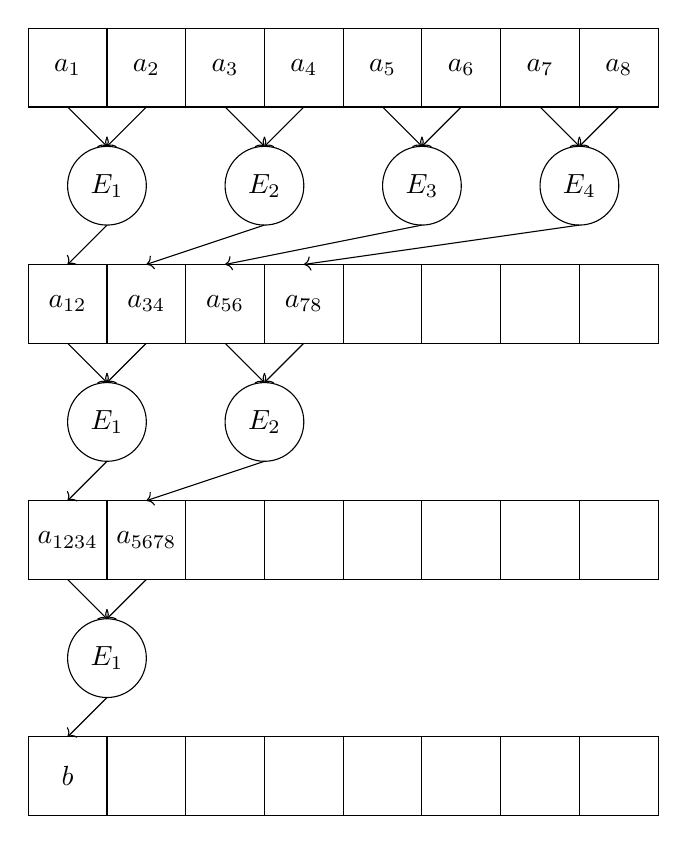
\begin{tikzpicture}
        \draw (0.0, 0.0) rectangle (1.0, -1.0) node [pos = 0.5] {$a_1$};
        \draw (1.0, 0.0) rectangle (2.0, -1.0) node [pos = 0.5] {$a_2$};
        \draw (2.0, 0.0) rectangle (3.0, -1.0) node [pos = 0.5] {$a_3$};
        \draw (3.0, 0.0) rectangle (4.0, -1.0) node [pos = 0.5] {$a_4$};
        \draw (4.0, 0.0) rectangle (5.0, -1.0) node [pos = 0.5] {$a_5$};
        \draw (5.0, 0.0) rectangle (6.0, -1.0) node [pos = 0.5] {$a_6$};
        \draw (6.0, 0.0) rectangle (7.0, -1.0) node [pos = 0.5] {$a_7$};
        \draw (7.0, 0.0) rectangle (8.0, -1.0) node [pos = 0.5] {$a_8$};

        \draw (1.0, -2.0) circle [radius = 0.50] node {$E_1$};
        \draw (3.0, -2.0) circle [radius = 0.50] node {$E_2$};
        \draw (5.0, -2.0) circle [radius = 0.50] node {$E_3$};
        \draw (7.0, -2.0) circle [radius = 0.50] node {$E_4$};

        \draw [->] (0.5, -1.0) -- (1.0, -1.5);
        \draw [->] (1.5, -1.0) -- (1.0, -1.5);
        \draw [->] (2.5, -1.0) -- (3.0, -1.5);
        \draw [->] (3.5, -1.0) -- (3.0, -1.5);
        \draw [->] (4.5, -1.0) -- (5.0, -1.5);
        \draw [->] (5.5, -1.0) -- (5.0, -1.5);
        \draw [->] (6.5, -1.0) -- (7.0, -1.5);
        \draw [->] (7.5, -1.0) -- (7.0, -1.5);

        \draw [->] (1.0, -2.5) -- (0.5, -3.0);
        \draw [->] (3.0, -2.5) -- (1.5, -3.0);
        \draw [->] (5.0, -2.5) -- (2.5, -3.0);
        \draw [->] (7.0, -2.5) -- (3.5, -3.0);

        \draw (0.0, -3.0) rectangle (1.0, -4.0) node [pos = 0.5] {$a_{12}$};
        \draw (1.0, -3.0) rectangle (2.0, -4.0) node [pos = 0.5] {$a_{34}$};
        \draw (2.0, -3.0) rectangle (3.0, -4.0) node [pos = 0.5] {$a_{56}$};
        \draw (3.0, -3.0) rectangle (4.0, -4.0) node [pos = 0.5] {$a_{78}$};
        \draw (4.0, -3.0) rectangle (5.0, -4.0);
        \draw (5.0, -3.0) rectangle (6.0, -4.0);
        \draw (6.0, -3.0) rectangle (7.0, -4.0);
        \draw (7.0, -3.0) rectangle (8.0, -4.0);

        \draw (1.0, -5.0) circle [radius = 0.50] node {$E_1$};
        \draw (3.0, -5.0) circle [radius = 0.50] node {$E_2$};

        \draw [->] (0.5, -4.0) -- (1.0, -4.5);
        \draw [->] (1.5, -4.0) -- (1.0, -4.5);
        \draw [->] (2.5, -4.0) -- (3.0, -4.5);
        \draw [->] (3.5, -4.0) -- (3.0, -4.5);

        \draw [->] (1.0, -5.5) -- (0.5, -6.0);
        \draw [->] (3.0, -5.5) -- (1.5, -6.0);

        \draw (0.0, -6.0) rectangle (1.0, -7.0) node [pos = 0.5] {$a_{1234}$};
        \draw (1.0, -6.0) rectangle (2.0, -7.0) node [pos = 0.5] {$a_{5678}$};
        \draw (2.0, -6.0) rectangle (3.0, -7.0);
        \draw (3.0, -6.0) rectangle (4.0, -7.0);
        \draw (4.0, -6.0) rectangle (5.0, -7.0);
        \draw (5.0, -6.0) rectangle (6.0, -7.0);
        \draw (6.0, -6.0) rectangle (7.0, -7.0);
        \draw (7.0, -6.0) rectangle (8.0, -7.0);

        \draw (1.0, -8.0) circle [radius = 0.50] node {$E_1$};

        \draw [->] (0.5, -7.0) -- (1.0, -7.5);
        \draw [->] (1.5, -7.0) -- (1.0, -7.5);

        \draw [->] (1.0, -8.5) -- (0.5, -9.0);

        \draw (0.0, -9.0) rectangle (1.0, -10.0) node [pos = 0.5] {$b$};
        \draw (1.0, -9.0) rectangle (2.0, -10.0);
        \draw (2.0, -9.0) rectangle (3.0, -10.0);
        \draw (3.0, -9.0) rectangle (4.0, -10.0);
        \draw (4.0, -9.0) rectangle (5.0, -10.0);
        \draw (5.0, -9.0) rectangle (6.0, -10.0);
        \draw (6.0, -9.0) rectangle (7.0, -10.0);
        \draw (7.0, -9.0) rectangle (8.0, -10.0);
    \end{tikzpicture}
    \caption{Visualisierung einer parallelen Reduktion}
    \label{methoden:reduction:viz}
\end{figure}

\subsubsection{GPU-Implementierung}

Im \gls{gpgpu}-Kontext ist die Reduktion früh untersucht worden. So stellte
Harris 2007 eine optimierte Reduktion für CUDA vor (vgl.~\cite{harris2007}). 
Eine für NVIDIAs Kepler-Architektur optimierte Variante der Reduktion wurde 2014
von Luitjens präsentiert (vgl.~\cite{luitjens2014}). Da sich Luitjens'
Implementierung NVIDIA-spezifischer Hardware-Intrinsiken bedient, die nicht auf
jeder im Rahmen dieser Arbeit untersuchten Plattform verfügbar sind, wird hier
ein anderer Ansatz verwendet.

Der Kernel, der die Reduktion durchführt, besteht aus zwei Stufen. Während der
ersten Stufe iterieren $x$ Arbeitsgruppen mit jeweils $p$ Arbeitseinheiten über
den globalen Speicher mit $n$ Elementen. Die Arbeitseinheiten führen die
Reduktion für jedes Elementepaar aus, wobei jeder Iterationsschritt $x \cdot p$
Elemente vom vorherigen Schritt entfernt auf den Speicher zugreift. Unter der
Annahme, dass $n$ ein Vielfaches von $p$ ist, werden $y = \frac{n}{p}$
Arbeitsgruppen gebraucht. Gilt $x \leq y$ unter der Bedingung, dass $y$ ein
Vielfaches von $x$ ist, führt jede Arbeitseinheit die Reduktionsoperation im
ersten Schritt genau $y$-mal aus. Dieses Zugriffsmuster ist als
\textit{(grid-)stride loop} bekannt und ein häufig genutztes Konzept der
\gls{gpgpu}-Programmierung (vgl.~\cite{harris2013} für eine Einführung und
Erklärung der Vorteile).

Während der zweiten Stufe werden die bisherigen Ergebnisse der einzelnen
Arbeitseinheiten in den lokalen Speicher geladen. Dann führt die Hälfte der
Arbeitseinheiten die Reduktionsoperation auf jeweils einem Elementepaar des
lokalen Speichers aus, dann ein Viertel auf der Arbeitseinheiten auf den neuen
Ergebnissen, usw. Am Ende gibt es pro Arbeitsgruppe genau ein Teilergebnis der
Reduktionsoperation (also $x$ Ergebnisse), das wieder in den globalen Speicher
geschrieben wird.

Durch einen erneuten Aufruf des Kernels mit einer Arbeitsgruppe und
$\frac{x}{2}$ Arbeitseinheiten lässt sich in einem weiteren Schritt das
Gesamtergebnis der Reduktion berechnen. Quelltext~\ref{methoden:reduction:code}
zeigt den Pseudo-Code des Kernels.

\begin{code}
    \begin{minted}[breaklines,breakafter=\,,escapeinside=||,fontsize=\small]{c++}
void block_reduce(const int* data, int* result, size_t num_elems)
{
    |\textbf{\textcolor{keyword-green}{local}}| int shared[p];

    int global_id = |\textbf{\textcolor{keyword-green}{group\_idx}}| * |\textbf{\textcolor{keyword-green}{group\_dim}}| + |\textbf{\textcolor{keyword-green}{unit\_idx}}|;
    int tsum = data[global_id]; // vermeide neutrales Element
    int grid_size = |\textbf{\textcolor{keyword-green}{group\_dim}}| * |\textbf{\textcolor{keyword-green}{num\_blocks}}|;
    global_id += grid_size;

    // 1. Stufe: grid-stride loop
    while((global_id + 3 * grid_size) < num_elems)
    {
        tsum += data[global_id] + data[global_id + grid_size] +
                data[global_id + 2 * grid_size] +
                data[global_id + 3 * grid_size];
        i += 4 * grid_size;
    }

    // verbleibende Elemente, falls n kein Vielfaches von p ist
    while(global_id < num_elems)
    {
        tsum += data[global_id];
        global_id += grid_size;
    }

    // schreibe Ergebnis in lokalen Speicher
    shared[|\textbf{\textcolor{keyword-green}{unit\_idx}}|] = tsum; 
    |\textbf{\textcolor{keyword-green}{synchronize}}|();

    // 2. Stufe: Reduktion innerhalb der Gruppe
    for(int bs = |\textbf{\textcolor{keyword-green}{group\_dim}}|, bsup = (|\textbf{\textcolor{keyword-green}{group\_dim}}| + 1) / 2;
        bs > 1;
        bs /= 2, bsup = (bs + 1) / 2)
    {
        bool cond = |\textbf{\textcolor{keyword-green}{unit\_idx}}| < bsup // erste Gruppenhälfte
            && |\textbf{\textcolor{keyword-green}{unit\_idx}}| + bsup < |\textbf{\textcolor{keyword-green}{group\_dim}}|
            && (|\textbf{\textcolor{keyword-green}{group\_idx}}| * |\textbf{\textcolor{keyword-green}{group\_dim}}| + |\textbf{\textcolor{keyword-green}{unit\_idx}}| + bsup) < num_elems;

        if(cond) shared[|\textbf{\textcolor{keyword-green}{unit\_idx}}|] += shared[|\textbf{\textcolor{keyword-green}{unit\_idx}}| + bsup];
        |\textbf{\textcolor{keyword-green}{synchronize}}|();
    }
    
    // Ergebnis in globalen Speicher schreiben
    if(|\textbf{\textcolor{keyword-green}{unit\_idx}}| == 0) result[|\textbf{\textcolor{keyword-green}{group\_idx}}|] = shared[0];
}
    \end{minted}
    \caption{Reduction-Benchmark}
    \label{methoden:reduction:code}
\end{code}

\subsection{N-Body-Benchmark}
\label{methoden:nbody}

\subsubsection{Vorbemerkung}
\label{methoden:nbody:vorbemerkung}

Eine effiziente Implementierung einer N-Body-Simulation mit quadratischer
Komplexität für GPUs wurde 2007 von Nyland et al.\ vorgestellt. Der in dieser
Arbeit verwendete Benchmark folgt dieser Implementierung, die theoretische
Beschreibung ist (gekürzt) ebenfalls der Arbeit von Nyland et al.\ entnommen.
(vgl.~\cite{nguyen2007})

\subsubsection{Einführung}
\label{methoden:nbody:einfuehrung}

N-Body-Simulationen wenden numerische Methoden an, um die Entwicklung eines
Systems vieler miteinander interagierender Körper zu approximieren.
N-Body-Probleme sind in den Naturwissenschaften zahlreich vertreten,
beispielsweise bei der Simulation vieler Galaxien oder Sterne und deren
Wechselwirkungen durch die Schwerkraft.

Eine N-Body-Simulation aller Körperpaare ist eine \textit{brute-force}-Technik,
die alle paarweisen Interaktionen auswertet. Aufgrund der quadratischen
Komplexität $\mathcal{O}(n^2)$ ist die Rechenlast bei großen Systemen sehr hoch:
ein System mit \num{16384} Körpern, das 20 Zeitschritte pro Sekunde simuliert,
berechnet über fünf Milliarden Interaktionen pro Sekunde. Aus diesem Grund ist
eine solche Simulation ein interessantes Ziel für den Einsatz paralleler
Beschleuniger.

\subsubsection{Mathematischer Hintergrund}
\label{methoden:nbody:mathematik}

In der in dieser Arbeit verwendeten Simulation wird das Gravitationspotential
aller Körper berechnet. Die in den folgenden Formeln vorkommenden Vektoren
werden in der Form $\vec{a}, \vec{b}, \vec{c}$ notiert und sind grundsätzlich
dreidimensional.

In einem System aus $N$ Körpern mit der Startposition $\vec{x}_i$ und der
Geschwindigkeit $\vec{v}_i$ ($1 \leq i \leq N$) ergibt sich die auf den Körper
$i$ durch die Anziehungskraft des Körpers $j$ wirkende Kraft $\vec{f}_{ij}$ wie
folgt:

\[
    \vec{f}_{ij} = G \frac{m_i m_j}{|\vec{r}_{ij}|^2} \cdot
                   \frac{\vec{r}_{ij}}{|\vec{r}_{ij}|},
\]

wobei $m_i$ und $m_j$ die Massen der Körper $i$ und $j$ sind,
$\vec{r}_{ij} = \vec{x}_j - \vec{x}_i$ der Vektor vom Körper $i$ zum Körper $j$
ist und $G$ die Gravitationskonstante darstellt. Der linke Faktor -- der
\textit{Betrag} der Kraft -- ist proportional zum Produkt der Massen und
schrumpft mit zunehmendem Abstand zwischen den Körpern $i$ und $j$. Der rechte
Faktor ist die \textit{Richtung} der Kraft. Aufgrund der anziehenden Wirkung
zwischen den Körpern $i$ und $j$ ist dieser Vektor ist ein Einheitsvektor.

Die gesamte auf den Körper $i$ wirkende Kraft $\vec{F}_i$, die sich aus den
Interaktionen mit den anderen $N - 1$ Körpern ergibt, ist die Summe aller
Interaktionen:

\[
    \vec{F}_i = \sum\limits_{\substack{1 \leq j \leq N\\ j \neq i}} \vec{f}_{ij}
              = G m_i \cdot \sum\limits_{\substack{1 \leq j \leq N\\j \neq i}}
                \frac{m_j \vec{r}_{ij}}{|\vec{r}_{ij}|^3}.
\]

Wenn sich Körper einander nähern, wächst die zwischen ihnen wirkende Kraft bis
ins Unendliche, was bei der numerischen Integration unerwünscht ist. In
astrophysikalischen Simulationen werden daher Kollisionen zwischen Körpern
grundsätzlich ausgeschlossen. Aus diesem Grund wird ein Schwächungsfaktor
$\varepsilon^2 > 0$ hinzugefügt und der Nenner wie folgt umgeschrieben:

\[
    \vec{F}_i \approx G m_i \cdot \sum\limits_{1 \leq j \leq N}
                      \frac{m_j \vec{r}_{ij}}
                           {\sqrt{|\vec{r}_{ij}|^2 + \varepsilon^2}^3}.
\]

Die Bedingung $j \neq i$ wird bei der Summe nicht länger benötigt, da
$\vec{f}_{ii} = 0$, wenn $\varepsilon^2 > 0$. Der Schwächungsfaktor stellt die
Interaktion zwischen zwei Plummer-Massepunkten dar, also Massen, die sich wie
kugelförmige Galaxien verhalten (vgl.~\cite{aarseth2003} und \cite{dyer1993}).
Effektiv beschränkt der Schwächungsfaktor die Größe der Kräfte zwischen Körpern,
was bei der numerischen Integration wünschenswert ist.

Um über die Zeit zu integrieren, muss die Beschleunigung
$\vec{a}_i = \frac{\vec{F}_i}{m_i}$ auf die Position und Geschwindigkeit des
Körpers $i$ angewendet werden, wodurch sich die Berechnung weiter vereinfacht:

\[
    \vec{a}_i \approx G \cdot \sum\limits_{1 \leq j \leq N}
                      \frac{m_j \vec{r}_{ij}}
                           {\sqrt{|\vec{r}_{ij}|^2 + \varepsilon^2}^3}
\]

Der numerische Integrator, der die Positionen und Geschwindigkeiten
aktualisiert und auch in dieser Arbeit zum Einsatz kommt, ist ein
Leapfrog-Verlet-Integrator (vgl.~\cite{verlet1967}). Er ist auf dieses Problem
anwendbar und berechnungseffizient, d.h. die Genauigkeit ist im Verhältnis zum
Rechenaufwand hoch. Die Wahl der Integrationsmethode für N-Body-Simulationen
hängt vom beobachteten System ab. Der Integrator wird in den Messungen mit
erfasst, in dieser Arbeit jedoch nicht gesondert beschrieben, da er eine lineare
Komplexität von $\mathcal{O}(n)$ besitzt und mit zunehmendem $n$ bedeutungslos
wird.

\subsubsection{GPU-Implementierung}
\label{methoden:nbody:gpu}

Den vorgestellten Algorithmus kann man sich als Berechnung jedes Feldes
$\vec{f}_{ij}$ in einem Gitter der Größe $N \times N$ vorstellen. In diesem Fall
ist die Gesamtkraft $\vec{F}_i$ bzw.\ die Beschleunigung $\vec{a}_i$ eines
Körpers $i$ die Summe aller Einträge der Zeile $i$. Jeder Eintrag kann
unabhängig von den anderen berechnet werden, was einen möglichen
Parallelisierungsgrad von $\mathcal{O}(n^2)$ ergibt. Dieser Ansatz hätte eine
Speicherkomplexität von ebenfalls $\mathcal{O}(n^2)$ zur Folge, was die
Performanz durch die verfügbare Speicherbandbreite limitieren würde. Stattdessen
werden einige Berechnungen serialisiert, um durch die Wiederverwendungen von
Daten die benötigte Speicherbandbreite zu verringern und die höchstmögliche
Leistung der arithmetischen Einheiten zu erreichen.

Das Gitter wird dazu in quadratische Kacheln gleicher Größe aufgeteilt, die aus
$p$ Zeilen und $p$ Spalten bestehen. $2p$ Körperbeschreibungen werden benötigt,
um alle $p^2$ Interaktionen innerhalb der Kachel zu berechnen, von denen $p$
wiederverwendet werden können. Diese Beschreibungen können dadurch im lokalen
Speicher oder in den Registern der auf der GPU verbauten Multiprozessoren
gehalten werden. Der Effekt der Interaktionen auf die $p$ Körper innerhalb der
Kachel wird als Aktualisierung von $p$ Beschleunigungsvektoren gespeichert.

Um die Daten effizient wiederverwenden zu können, erfolgen die Berechnungen
in einer Zeile in sequentieller Reihenfolge, während die einzelnen Zeilen
parallel berechnet werden. Abbildung~\ref{methoden:nbody:gpu:kacheln} zeigt
links die Ausführungsstrategie und rechts die Ein- und Ausgabewerte einer
Kachel.

\begin{figure}[htb]
    \centering
    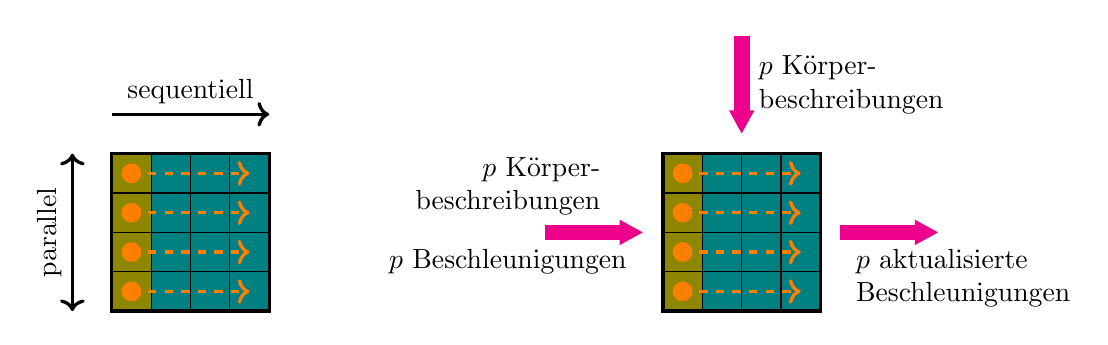
\begin{tikzpicture}
        %
        % ERSTES QUADRAT
        %

        % Farbe
        \fill [color = olive] (0.5, -0.5) rectangle (1.0, -2.5); % erste Spalte
        \fill [color = teal] (1.0, -0.5) rectangle (2.5, -2.5); % Rest

        % Rand
        \draw [line width = 1.2pt] (0.5, -0.5) rectangle (2.5, -2.5);

        % Zeilen
        \draw (0.5, -1.0) -- (2.5, -1.0); % Erste Zeile
        \draw (0.5, -1.5) -- (2.5, -1.5); % Zweite Zeile
        \draw (0.5, -2.0) -- (2.5, -2.0); % Dritte Zeile

        % Spalten
        \draw (1.0, -0.5) -- (1.0, -2.5); % Erste Spalte
        \draw (1.5, -0.5) -- (1.5, -2.5); % Zweite Spalte
        \draw (2.0, -0.5) -- (2.0, -2.5); % Dritte Spalte

        % Beschriftung oben
        \draw [->, line width = 1.2pt]
              (0.5, 0.0) -- (2.5, 0.0)
              node[pos = 0.5, align = center, above] {sequentiell};

        % Beschriftung links
        \draw [<->, line width = 1.2pt]
              (0.0, -2.5) -- (0.0, -0.5)
              node[pos = 0.5, align = center, above, sloped] {parallel};

        % Pfeil - erste Zeile
        \draw [->, dashed, line width = 1.2pt, draw = orange]
              (0.75, -0.75) -- (2.25, -0.75);
        \fill [color = orange] (0.75, -0.75) circle [radius = 0.125];

        % Pfeil - zweite Zeile
        \draw [->, dashed, line width = 1.2pt, draw = orange]
              (0.75, -1.25) -- (2.25, -1.25);
        \fill [color = orange] (0.75, -1.25) circle [radius = 0.125];

        % Pfeil - erste Zeile
        \draw [->, dashed, line width = 1.2pt, draw = orange]
              (0.75, -1.75) -- (2.25, -1.75);
        \fill [color = orange] (0.75, -1.75) circle [radius = 0.125];

        % Pfeil - erste Zeile
        \draw [->, dashed, line width = 1.2pt, draw = orange]
              (0.75, -2.25) -- (2.25, -2.25);
        \fill [color = orange] (0.75, -2.25) circle [radius = 0.125];

        %
        % ZWEITES QUADRAT
        %

        % Farbe
        \fill [color = olive] (7.5, -0.5) rectangle (8.0, -2.5); % erste Spalte
        \fill [color = teal] (8.0, -0.5) rectangle (9.5, -2.5); % Rest

        % Rand
        \draw [line width = 1.2pt] (7.5, -0.5) rectangle (9.5, -2.5);

        % Zeilen
        \draw (7.5, -1.0) -- (9.5, -1.0); % Erste Zeile
        \draw (7.5, -1.5) -- (9.5, -1.5); % Zweite Zeile
        \draw (7.5, -2.0) -- (9.5, -2.0); % Dritte Zeile

        % Spalten
        \draw (8.0, -0.5) -- (8.0, -2.5); % Erste Spalte
        \draw (8.5, -0.5) -- (8.5, -2.5); % Zweite Spalte
        \draw (9.0, -0.5) -- (9.0, -2.5); % Dritte Spalte

        % Beschriftung oben
        \draw [->, >={Triangle[width=3mm,length=3mm]}, color = magenta,
               line width = 2mm, text = black]
              (8.5, 1.0) -- (8.5, -0.25)
              node [pos = 0.5, right, align = left]
              {$p$ Körper- \\ beschreibungen};

        % Beschriftung links
        \draw [->, >={Triangle[width=3mm,length=3mm]}, color = magenta,
               line width = 2mm, text = black]
              (6.0, -1.5) -- (7.25, -1.5)

              node [pos = -0.375, above, align = right]
              {$p$ Körper-\\beschreibungen}

              node [pos = -0.375, below] {$p$ Beschleunigungen};

        % Beschriftung rechts
        \draw [->, >={Triangle[width=3mm,length=3mm]}, color = magenta,
               line width = 2mm, text = black]
              (9.75, -1.5) -- (11.0, -1.5)

              node [pos = 1.25, below, align = left]
              {$p$ aktualisierte\\Beschleunigungen};

        % Pfeil - erste Zeile
        \draw [->, dashed, line width = 1.2pt, draw = orange]
              (7.75, -0.75) -- (9.25, -0.75);
        \fill [color = orange] (7.75, -0.75) circle [radius = 0.125];

        % Pfeil - zweite Zeile
        \draw [->, dashed, line width = 1.2pt, draw = orange]
              (7.75, -1.25) -- (9.25, -1.25);
        \fill [color = orange] (7.75, -1.25) circle [radius = 0.125];

        % Pfeil - erste Zeile
        \draw [->, dashed, line width = 1.2pt, draw = orange]
              (7.75, -1.75) -- (9.25, -1.75);
        \fill [color = orange] (7.75, -1.75) circle [radius = 0.125];

        % Pfeil - erste Zeile
        \draw [->, dashed, line width = 1.2pt, draw = orange]
              (7.75, -2.25) -- (9.25, -2.25);
        \fill [color = orange] (7.75, -2.25) circle [radius = 0.125];
    \end{tikzpicture}
    \caption{Schema einer Kachel}
    \label{methoden:nbody:gpu:kacheln}
\end{figure}

Der Pseudo-Code in Quelltext~\ref{methoden:nbody:gpu:bodybodyinteraction}
dient der Berechnung der Krafteinwirkung auf einen Körper $i$ durch die
Interaktion mit dem Körper $j$ und aktualisiert die Beschleunigung $a_i$ des
Körpers $i$. Die Beschreibungen der Körper enthalten die Koordinaten in den
Feldern \texttt{x}, \texttt{y} und \texttt{z} sowie die Körpermasse im Feld
\texttt{w}. Die Berechnung einer Interaktion benötigt 20 \glspl{flop}.

\begin{code}
    \begin{minted}[breaklines,breakafter=\,,escapeinside=||,fontsize=\small]{c++}
const float epsilon2 = epsilon * epsilon;

float3 body_body_interaction(float4 i, float4 j, float3 ai)
{
    // 3 FLOPs
    float3 r = j.xyz - i.xyz;

    // 6 FLOPs
    float dist_sqr = skalarprodukt(r, r) + epsilon2;

    // 4 FLOPs (2x Multiplikation, Wurzel, Inversion 
    float inv_dist_cube = 1.0 / sqrt(dist_sqr * dist_sqr * dist_sqr);

    // 1 FLOP
    float s = j.w * inv_dist_cube;

    // 6 FLOPs -- ai und r sind Vektoren, s ist skalar
    ai += r * s;

    return ai;
}
    \end{minted}
    \caption{Berechnung der Interaktion zwischen zwei Körpern}
    \label{methoden:nbody:gpu:bodybodyinteraction}
\end{code}

Eine Kachel wird von $p$ Threads ausgewertet, wobei jeder Thread die
Beschleunigung eines Körpers als Ergebnis seiner Interaktion mit $p$ anderen
Körpern aktualisiert. Das heißt, dass $p$ Körperbeschreibungen aus dem globalen
Speicher der GPU in den lokalen Speicher des Multiprozessors geladen werden.
Jeder Thread innerhalb des Blocks wertet $p$ aufeinanderfolgende Interaktionen
aus, was $p$ aktualisierte Beschleunigungen ergibt. Der Pseudo-Code in
Quelltext~\ref{methoden:nbody:gpu:tilecalculation} zeigt diese Berechnung. Der
Parameter \texttt{my\_position} enthält die Position des Körpers, den der
aktuelle Thread auswertet, während das im lokalen Speicher liegende Array
\texttt{sh\_position} die Beschreibungen der $p$ interagierenden Körper enthält.

\begin{code}
    \begin{minted}[breaklines,breakafter=\,,escapeinside=||,fontsize=\small]
          {c++}
float3 tile_calculation(float4 my_position, float3 accel)
{
    |\textbf{\textcolor{keyword-green}{local}}| float4 sh_position[p];
    for(int i = 0; i < p; ++i)
        accel = body_body_interaction(my_position, sh_position[i],
                                      accel);

    return accel;
}
    \end{minted}
    \caption{Berechnung der Interaktionen einer Kachel mit $p \times p$
             Elementen}
    \label{methoden:nbody:gpu:tilecalculation}
\end{code}

Im hier verwendeten Benchmark verarbeitet eine Gruppe von $p$ Arbeitseinheiten
sequentiell eine Reihe von $\frac{N}{p}$ Kacheln der Größe $p \times p$. Die
Wiederverwendung von Daten wird effektiver, je länger eine Zeile wird. Die
Zeilenlänge beeinflusst gleichzeitig die Größe der aus dem globalen in den
lokalen Speicher kopierten Daten. Die Kachelgröße selbst bestimmt somit den
Bedarf an Registern und lokalem Speicher. Vor der Verarbeitung einer Kachel lädt
jede Arbeitseinheit einen Körper in den lokalen Speicher und synchronisiert mit
den anderen Arbeitseinheiten innerhalb der Arbeitsgruppe. Somit liegen vor der
Verarbeitung jeder Kachel $p$ aufeinanderfolgende Körper im lokalen Speicher.

Die Abbildung~\ref{methoden:nbody:gpu:tilecluster} zeigt eine Arbeitsgruppe,
die nacheinander mehrere Kacheln verarbeitet. In horizontaler Richtung erstreckt
sich die Zeit, während die Parallelität in vertikaler Richtung zu sehen ist. Die
fett gezeichneten Linien rahmen die Kacheln ein und zeigen gleichzeitig die
Zeitpunkte, an denen der lokale Speicher befüllt wird und die Synchronisierung
der Arbeitseinheiten erfolgt. Alle $p$ Arbeitseinheiten einer Gruppe berechnen
innerhalb einer Kachel die Kräfte, die auf $p$ Körper wirken (eine Einheit pro
Körper); bei $\frac{N}{p}$ Kacheln pro Arbeitsgruppe berechnet damit jede
Einheit alle $N$ Interaktionen pro Körper.

\begin{figure}[htb]
    \centering
    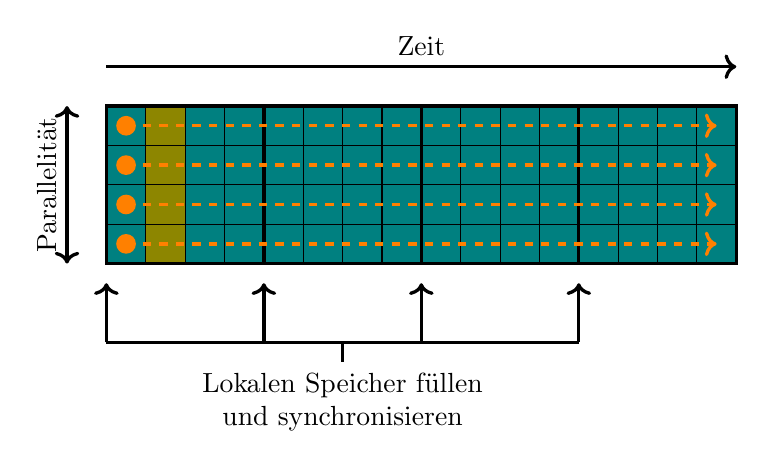
\begin{tikzpicture}
        % Farbe
        \fill [color = teal] (0.5, -0.5) rectangle (8.5, -2.5); % alles
        \fill [color = olive] (1.0, -0.5) rectangle (1.5, -2.5); % zweite Spalte

        % Rand
        \draw [line width = 1.2pt] (0.5, -0.5) rectangle (8.5, -2.5);

        % Zeilen
        \draw (0.5, -1.0) -- (8.5, -1.0); % Erste Zeile
        \draw (0.5, -1.5) -- (8.5, -1.5); % Zweite Zeile
        \draw (0.5, -2.0) -- (8.5, -2.0); % Dritte Zeile

        % Spalten
        \draw (1.0, -0.5) -- (1.0, -2.5); % Erste Spalte  (1. Q)
        \draw (1.5, -0.5) -- (1.5, -2.5); % Zweite Spalte (1. Q)
        \draw (2.0, -0.5) -- (2.0, -2.5); % Dritte Spalte (1. Q)

        \draw [line width = 1.2pt] (2.5, -0.5) -- (2.5, -2.5); % Sync #1
        
        \draw (3.0, -0.5) -- (3.0, -2.5); % Erste Spalte  (2. Q)
        \draw (3.5, -0.5) -- (3.5, -2.5); % Zweite Spalte (2. Q)
        \draw (4.0, -0.5) -- (4.0, -2.5); % Dritte Spalte (2. Q)

        \draw [line width = 1.2pt] (4.5, -0.5) -- (4.5, -2.5); % Sync #2

        \draw (5.0, -0.5) -- (5.0, -2.5); % Erste Spalte  (3. Q)
        \draw (5.5, -0.5) -- (5.5, -2.5); % Zweite Spalte (3. Q)
        \draw (6.0, -0.5) -- (6.0, -2.5); % Dritte Spalte (3. Q)

        \draw [line width = 1.2pt] (6.5, -0.5) -- (6.5, -2.5); % Sync #3

        \draw (7.0, -0.5) -- (7.0, -2.5); % Erste Spalte  (4. Q)
        \draw (7.5, -0.5) -- (7.5, -2.5); % Zweite Spalte (4. Q)
        \draw (8.0, -0.5) -- (8.0, -2.5); % Dritte Spalte (4. Q)

        % Spalten

        % Pfeil - erste Zeile
        \draw [->, dashed, line width = 1.2pt, draw = orange]
              (0.75, -0.75) -- (8.25, -0.75);
        \fill [color = orange] (0.75, -0.75) circle [radius = 0.125];

        % Pfeil - zweite Zeile
        \draw [->, dashed, line width = 1.2pt, draw = orange]
              (0.75, -1.25) -- (8.25, -1.25);
        \fill [color = orange] (0.75, -1.25) circle [radius = 0.125];

        % Pfeil - erste Zeile
        \draw [->, dashed, line width = 1.2pt, draw = orange]
              (0.75, -1.75) -- (8.25, -1.75);
        \fill [color = orange] (0.75, -1.75) circle [radius = 0.125];

        % Pfeil - erste Zeile
        \draw [->, dashed, line width = 1.2pt, draw = orange]
              (0.75, -2.25) -- (8.25, -2.25);
        \fill [color = orange] (0.75, -2.25) circle [radius = 0.125];

        % Beschriftung oben
        \draw [->, line width = 1.2pt] (0.5, 0.0) -- (8.5, 0.0)
              node [pos = 0.5, align = center, above] {Zeit};

        % Beschriftung links
        \draw [<->, line width = 1.2pt]
              (0.0, -2.5) -- (0.0, -0.5)
              node[pos = 0.5, align = center, above, sloped] {Parallelität};

        % Beschriftung unten
        \draw [line width = 1.2pt] (0.5, -3.5) -- (6.5, -3.5);
        \draw [->, line width = 1.2pt] (0.5, -3.5) -- (0.5, -2.75);
        \draw [->, line width = 1.2pt] (2.5, -3.5) -- (2.5, -2.75);
        \draw [->, line width = 1.2pt] (4.5, -3.5) -- (4.5, -2.75);
        \draw [->, line width = 1.2pt] (6.5, -3.5) -- (6.5, -2.75);
        \draw [line width = 1.2pt] (3.5, -3.5) -- (3.5, -3.75)
              node [pos = 1.0, align = center, below] {Lokalen Speicher füllen\\
              und synchronisieren};
    \end{tikzpicture}
    \caption{Berechnungen einer Arbeitsgruppe}
    \label{methoden:nbody:gpu:tilecluster}
\end{figure}

Quelltext~\ref{methoden:nbody:gpu:calcforces} zeigt den Pseudo-Code, der diese
Berechnung für GPUs umsetzt. Die Parameter \texttt{x} und \texttt{a} sind
Zeiger auf den globalen Speicher und enthalten die Positionen (\texttt{x}) und
Beschleunigungen (\texttt{a}) der Körper. Die Iteration über die Kacheln
erfordert zwei Synchronisierungspunkte. Der Erste stellt sicher, dass alle
Felder des lokalen Speichers befüllt wurden, bevor die Berechnung beginnt. Der
zweite Synchronisationspunkt garantiert, dass alle Berechnungen abgeschlossen
wurden, bevor die nächste Kachel verarbeitet wird.

\begin{code}
    \begin{minted}[breaklines,breakafter=\,,escapeinside=||,fontsize=\small]
          {c++}
void tile_calculation(float4* x, float3* a)
{
    |\textbf{\textcolor{keyword-green}{local}}| float4 sh_position[p];

    float3 acc = {0.0, 0.0, 0.0};
    int global_id = |\textbf{\textcolor{keyword-green}{group\_idx}}| * |\textbf{\textcolor{keyword-green}{group\_dim}}| + |\textbf{\textcolor{keyword-green}{unit\_idx}}|;

    float4 my_position = x[global_id];

    for(int i = 0, tile = 0; i < N; i += p, ++tile)
    {
        int idx = tile * |\textbf{\textcolor{keyword-green}{group\_dim}}| + |\textbf{\textcolor{keyword-green}{unit\_idx}}|;
        sh_position[|\textbf{\textcolor{keyword-green}{unit\_idx}}|] = x[idx];
        |\textbf{\textcolor{keyword-green}{synchronize}}|();

        acc = tile_calculation(my_position, acc);
        |\textbf{\textcolor{keyword-green}{synchronize}}|();
    }

    // Ergebnis für folgenden Integrationsschritt abspeichern
    a[global_id] = acc;
}
    \end{minted}
    \caption{Berechnung aller $N$ Interaktionen für $p$ Körper innerhalb einer
             Arbeitsgruppe mit $p$ Arbeitseinheiten}
    \label{methoden:nbody:gpu:calcforces}
\end{code}

Der gezeigte Pseudo-Code berechnet die Beschleunigung von $p$ Körpern eines
Systems, die durch ihre Interaktion mit allen $N$ Körpern im System
hervorgerufen wird. Um die Beschleunigung aller $N$ Körper zu berechnen, werden
mehrere Arbeitsgruppen eingesetzt. Da es $p$ Arbeitseinheiten pro Arbeitsgruppe
und eine Arbeitseinheit pro Körper gibt, ist die Zahl der benötigten
Arbeitsgruppen $\frac{N}{p}$. Im Gesamtsystem gibt es somit $N$
Arbeitseinheiten, die jeweils $N$ Berechnungen durchführen. Insgesamt werden
auf diese Weise $N^2$ Interaktionen berechnet. Eine Visualisierung dieses
Vorgangs findet sich in Abbildung~\ref{methoden:nbody:gpu:grid}. Die vertikale
Dimension zeigt die Parallelisierung, die durch $\frac{N}{p}$ unabhängige
Arbeitsgruppen mit jeweils $p$ Arbeitseinheiten erreicht wird. Die horizontale
Dimension zeigt die sequentielle Verarbeitung von $N$ Berechnungen durch jede
Arbeitseinheit. Eine Arbeitsgruppe lädt ihren lokalen Speicher alle $p$ Schritte
neu, um $p$ Positionen zu teilen.

\begin{figure}[htb]
    \centering
    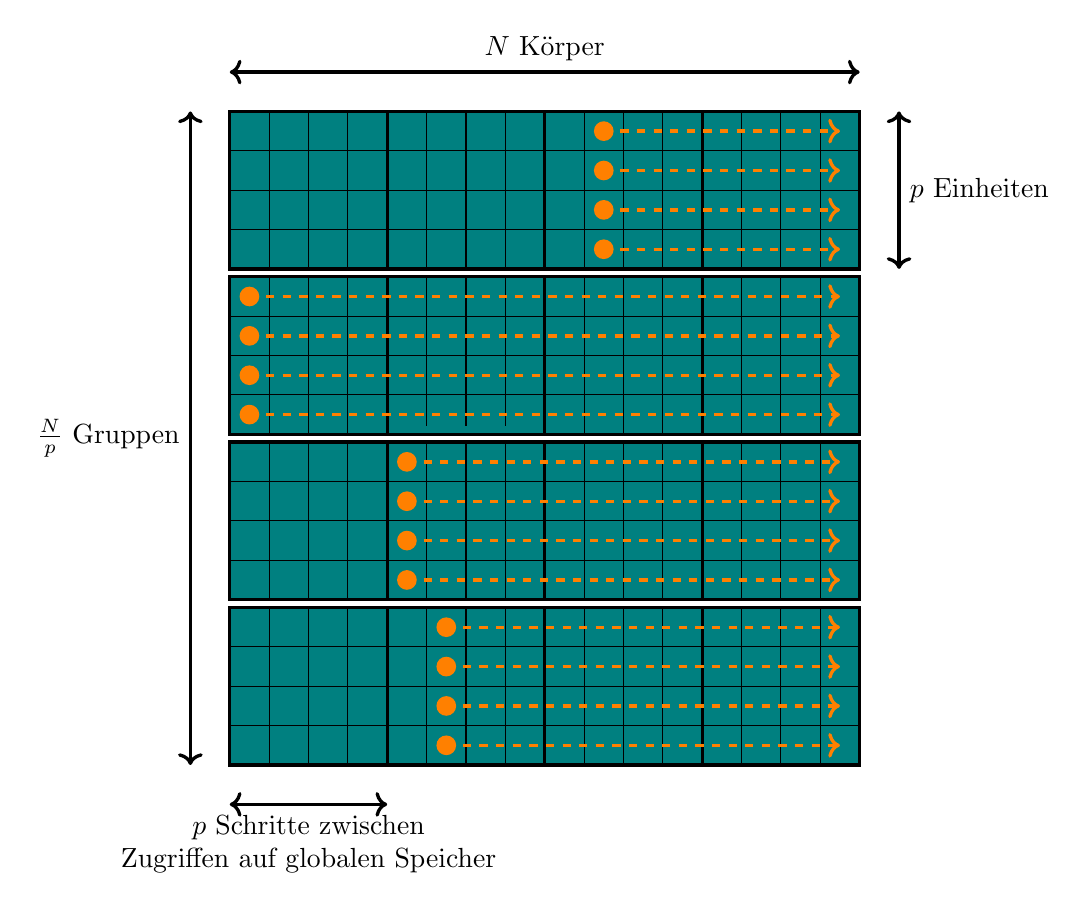
\begin{tikzpicture}
        %
        % ERSTE GRUPPE
        %

        % Farbe
        \fill [color = teal] (0.5, -0.5) rectangle (8.5, -2.5); % alles

        % Rand
        \draw [line width = 1.2pt] (0.5, -0.5) rectangle (8.5, -2.5);

        % Zeilen
        \draw (0.5, -1.0) -- (8.5, -1.0); % Erste Zeile
        \draw (0.5, -1.5) -- (8.5, -1.5); % Zweite Zeile
        \draw (0.5, -2.0) -- (8.5, -2.0); % Dritte Zeile

        % Spalten
        \draw (1.0, -0.5) -- (1.0, -2.5); % Erste Spalte  (1. Q)
        \draw (1.5, -0.5) -- (1.5, -2.5); % Zweite Spalte (1. Q)
        \draw (2.0, -0.5) -- (2.0, -2.5); % Dritte Spalte (1. Q)

        \draw [line width = 1.2pt] (2.5, -0.5) -- (2.5, -2.5); % Sync #1
        
        \draw (3.0, -0.5) -- (3.0, -2.5); % Erste Spalte  (2. Q)
        \draw (3.5, -0.5) -- (3.5, -2.5); % Zweite Spalte (2. Q)
        \draw (4.0, -0.5) -- (4.0, -2.5); % Dritte Spalte (2. Q)

        \draw [line width = 1.2pt] (4.5, -0.5) -- (4.5, -2.5); % Sync #2

        \draw (5.0, -0.5) -- (5.0, -2.5); % Erste Spalte  (3. Q)
        \draw (5.5, -0.5) -- (5.5, -2.5); % Zweite Spalte (3. Q)
        \draw (6.0, -0.5) -- (6.0, -2.5); % Dritte Spalte (3. Q)

        \draw [line width = 1.2pt] (6.5, -0.5) -- (6.5, -2.5); % Sync #3

        \draw (7.0, -0.5) -- (7.0, -2.5); % Erste Spalte  (4. Q)
        \draw (7.5, -0.5) -- (7.5, -2.5); % Zweite Spalte (4. Q)
        \draw (8.0, -0.5) -- (8.0, -2.5); % Dritte Spalte (4. Q)

        % Pfeil - erste Zeile
        \draw [->, dashed, line width = 1.2pt, draw = orange]
              (5.25, -0.75) -- (8.25, -0.75);
        \fill [color = orange] (5.25, -0.75) circle [radius = 0.125];

        % Pfeil - zweite Zeile
        \draw [->, dashed, line width = 1.2pt, draw = orange]
              (5.25, -1.25) -- (8.25, -1.25);
        \fill [color = orange] (5.25, -1.25) circle [radius = 0.125];

        % Pfeil - dritte Zeile
        \draw [->, dashed, line width = 1.2pt, draw = orange]
              (5.25, -1.75) -- (8.25, -1.75);
        \fill [color = orange] (5.25, -1.75) circle [radius = 0.125];

        % Pfeil - vierte Zeile
        \draw [->, dashed, line width = 1.2pt, draw = orange]
              (5.25, -2.25) -- (8.25, -2.25);
        \fill [color = orange] (5.25, -2.25) circle [radius = 0.125];

        %
        % ZWEITE GRUPPE
        %

        % Farbe
        \fill [color = teal] (0.5, -2.6) rectangle (8.5, -4.6);

        % Rand
        \draw [line width = 1.2pt] (0.5, -2.6) rectangle (8.5, -4.6);

        % Zeilen
        \draw (0.5, -3.1) -- (8.5, -3.1); % Erste Zeile
        \draw (0.5, -3.6) -- (8.5, -3.6); % Zweite Zeile
        \draw (0.5, -4.1) -- (8.5, -4.1); % Dritte Zeile

        % Spalten
        \draw (1.0, -2.6) -- (1.0, -4.6); % Erste Spalte  (1. Q)
        \draw (1.5, -2.6) -- (1.5, -4.6); % Zweite Spalte (1. Q)
        \draw (2.0, -2.6) -- (2.0, -4.6); % Dritte Spalte (1. Q)

        \draw [line width = 1.2pt] (2.5, -2.6) -- (2.5, -4.6); % Sync #1
        
        \draw (3.0, -2.6) -- (3.0, -4.5); % Erste Spalte  (2. Q)
        \draw (3.5, -2.6) -- (3.5, -4.5); % Zweite Spalte (2. Q)
        \draw (4.0, -2.6) -- (4.0, -4.5); % Dritte Spalte (2. Q)

        \draw [line width = 1.2pt] (4.5, -2.6) -- (4.5, -4.6); % Sync #2

        \draw (5.0, -2.6) -- (5.0, -4.6); % Erste Spalte  (3. Q)
        \draw (5.5, -2.6) -- (5.5, -4.6); % Zweite Spalte (3. Q)
        \draw (6.0, -2.6) -- (6.0, -4.6); % Dritte Spalte (3. Q)

        \draw [line width = 1.2pt] (6.5, -2.6) -- (6.5, -4.6); % Sync #3

        \draw (7.0, -2.6) -- (7.0, -4.6); % Erste Spalte  (4. Q)
        \draw (7.5, -2.6) -- (7.5, -4.6); % Zweite Spalte (4. Q)
        \draw (8.0, -2.6) -- (8.0, -4.6); % Dritte Spalte (4. Q)

        % Pfeil - erste Zeile
        \draw [->, dashed, line width = 1.2pt, draw = orange]
              (0.75, -2.85) -- (8.25, -2.85);
        \fill [color = orange] (0.75, -2.85) circle [radius = 0.125];

        % Pfeil - zweite Zeile
        \draw [->, dashed, line width = 1.2pt, draw = orange]
              (0.75, -3.35) -- (8.25, -3.35);
        \fill [color = orange] (0.75, -3.35) circle [radius = 0.125];

        % Pfeil - dritte Zeile
        \draw [->, dashed, line width = 1.2pt, draw = orange]
              (0.75, -3.85) -- (8.25, -3.85);
        \fill [color = orange] (0.75, -3.85) circle [radius = 0.125];

        % Pfeil - vierte Zeile
        \draw [->, dashed, line width = 1.2pt, draw = orange]
              (0.75, -4.35) -- (8.25, -4.35);
        \fill [color = orange] (0.75, -4.35) circle [radius = 0.125];

        %
        % DRITTE GRUPPE
        %

        % Farbe
        \fill [color = teal] (0.5, -4.7) rectangle (8.5, -6.7);

        % Rand
        \draw [line width = 1.2pt] (0.5, -4.7) rectangle (8.5, -6.7);

        % Zeilen
        \draw (0.5, -5.2) -- (8.5, -5.2); % Erste Zeile
        \draw (0.5, -5.7) -- (8.5, -5.7); % Zweite Zeile
        \draw (0.5, -6.2) -- (8.5, -6.2); % Dritte Zeile

        % Spalten
        \draw (1.0, -4.7) -- (1.0, -6.7); % Erste Spalte  (1. Q)
        \draw (1.5, -4.7) -- (1.5, -6.7); % Zweite Spalte (1. Q)
        \draw (2.0, -4.7) -- (2.0, -6.7); % Dritte Spalte (1. Q)

        \draw [line width = 1.2pt] (2.5, -4.7) -- (2.5, -6.7); % Sync #1
        
        \draw (3.0, -4.7) -- (3.0, -6.7); % Erste Spalte  (2. Q)
        \draw (3.5, -4.7) -- (3.5, -6.7); % Zweite Spalte (2. Q)
        \draw (4.0, -4.7) -- (4.0, -6.7); % Dritte Spalte (2. Q)

        \draw [line width = 1.2pt] (4.5, -4.7) -- (4.5, -6.7); % Sync #2

        \draw (5.0, -4.7) -- (5.0, -6.7); % Erste Spalte  (3. Q)
        \draw (5.5, -4.7) -- (5.5, -6.7); % Zweite Spalte (3. Q)
        \draw (6.0, -4.7) -- (6.0, -6.7); % Dritte Spalte (3. Q)

        \draw [line width = 1.2pt] (6.5, -4.7) -- (6.5, -6.7); % Sync #3

        \draw (7.0, -4.7) -- (7.0, -6.7); % Erste Spalte  (4. Q)
        \draw (7.5, -4.7) -- (7.5, -6.7); % Zweite Spalte (4. Q)
        \draw (8.0, -4.7) -- (8.0, -6.7); % Dritte Spalte (4. Q)

        % Pfeil - erste Zeile
        \draw [->, dashed, line width = 1.2pt, draw = orange]
              (2.75, -4.95) -- (8.25, -4.95);
        \fill [color = orange] (2.75, -4.95) circle [radius = 0.125];

        % Pfeil - zweite Zeile
        \draw [->, dashed, line width = 1.2pt, draw = orange]
              (2.75, -5.45) -- (8.25, -5.45);
        \fill [color = orange] (2.75, -5.45) circle [radius = 0.125];

        % Pfeil - dritte Zeile
        \draw [->, dashed, line width = 1.2pt, draw = orange]
              (2.75, -5.95) -- (8.25, -5.95);
        \fill [color = orange] (2.75, -5.95) circle [radius = 0.125];

        % Pfeil - vierte Zeile
        \draw [->, dashed, line width = 1.2pt, draw = orange]
              (2.75, -6.45) -- (8.25, -6.45);
        \fill [color = orange] (2.75, -6.45) circle [radius = 0.125];

        %
        % VIERTE GRUPPE
        %

        % Farbe
        \fill [color = teal] (0.5, -6.8) rectangle (8.5, -8.8);

        % Rand
        \draw [line width = 1.2pt] (0.5, -6.8) rectangle (8.5, -8.8);

        % Zeilen
        \draw (0.5, -7.3) -- (8.5, -7.3); % Erste Zeile
        \draw (0.5, -7.8) -- (8.5, -7.8); % Zweite Zeile
        \draw (0.5, -8.3) -- (8.5, -8.3); % Dritte Zeile

        % Spalten
        \draw (1.0, -6.8) -- (1.0, -8.8); % Erste Spalte  (1. Q)
        \draw (1.5, -6.8) -- (1.5, -8.8); % Zweite Spalte (1. Q)
        \draw (2.0, -6.8) -- (2.0, -8.8); % Dritte Spalte (1. Q)

        \draw [line width = 1.2pt] (2.5, -6.8) -- (2.5, -8.8); % Sync #1
        
        \draw (3.0, -6.8) -- (3.0, -8.8); % Erste Spalte  (2. Q)
        \draw (3.5, -6.8) -- (3.5, -8.8); % Zweite Spalte (2. Q)
        \draw (4.0, -6.8) -- (4.0, -8.8); % Dritte Spalte (2. Q)

        \draw [line width = 1.2pt] (4.5, -6.8) -- (4.5, -8.8); % Sync #2

        \draw (5.0, -6.8) -- (5.0, -8.8); % Erste Spalte  (3. Q)
        \draw (5.5, -6.8) -- (5.5, -8.8); % Zweite Spalte (3. Q)
        \draw (6.0, -6.8) -- (6.0, -8.8); % Dritte Spalte (3. Q)

        \draw [line width = 1.2pt] (6.5, -6.8) -- (6.5, -8.8); % Sync #3

        \draw (7.0, -6.8) -- (7.0, -8.8); % Erste Spalte  (4. Q)
        \draw (7.5, -6.8) -- (7.5, -8.8); % Zweite Spalte (4. Q)
        \draw (8.0, -6.8) -- (8.0, -8.8); % Dritte Spalte (4. Q)

        % Pfeil - erste Zeile
        \draw [->, dashed, line width = 1.2pt, draw = orange]
              (3.25, -7.05) -- (8.25, -7.05);
        \fill [color = orange] (3.25, -7.05) circle [radius = 0.125];

        % Pfeil - zweite Zeile
        \draw [->, dashed, line width = 1.2pt, draw = orange]
              (3.25, -7.55) -- (8.25, -7.55);
        \fill [color = orange] (3.25, -7.55) circle [radius = 0.125];

        % Pfeil - dritte Zeile
        \draw [->, dashed, line width = 1.2pt, draw = orange]
              (3.25, -8.05) -- (8.25, -8.05);
        \fill [color = orange] (3.25, -8.05) circle [radius = 0.125];

        % Pfeil - vierte Zeile
        \draw [->, dashed, line width = 1.2pt, draw = orange]
              (3.25, -8.55) -- (8.25, -8.55);
        \fill [color = orange] (3.25, -8.55) circle [radius = 0.125];

        % Beschriftung oben
        \draw [<->, line width = 1.2pt] (0.5, 0.0) -- (8.5, 0.0)
              node [pos = 0.5, align = center, above] {$N$ Körper};

        % Beschriftung links
        \draw [<->, line width = 1.2pt]
              (0.0, -8.8) -- (0.0, -0.5)
              node[pos = 0.5, left] {$\frac{N}{p}$ Gruppen};

        % Beschriftung unten
        \draw [<->, line width = 1.2pt]
              (0.5, -9.3) -- (2.5, -9.3)
              node[pos = 0.5, below, align = center]
              {$p$ Schritte zwischen\\Zugriffen auf globalen Speicher};

        % Beschriftung rechts
        \draw [<->, line width = 1.2pt]
              (9.0, -0.5) -- (9.0, -2.5)
              node[pos = 0.5, right] {$p$ Einheiten};
    \end{tikzpicture}
    \caption{Berechnung aller Interaktionen}
    \label{methoden:nbody:gpu:grid}
\end{figure}

\section{Messungen auf NVIDIA-GPUs}
\label{nvidia}

\subsection{Verwendete Hard- und Software}

Die hier gezeigten Benchmark-Ergebnisse wurden auf einem Knoten der
\texttt{gpu2}-Partition des \gls{hpc}-Systems Taurus gemessen, der über zwei
GPUs des Modells Tesla K20x (mit aktiviertem ECC) verfügt.

Die Messungen fanden innerhalb der SCS5-Umgebung statt, in der die folgende
Software verwendet wurde:

\begin{itemize}
    \item \texttt{CUDA/10.0.130} (Modulsystem)
    \item \texttt{GCC/7.3.0-2.30} (Modulsystem)
    \item \gls{hip} (Version 1.5.19061, ROCm-GitHub-Repository)
    \item ComputeCpp (Codeplays SYCL-Implementierung, Version 1.0.5 für Ubuntu
          14.04)
\end{itemize}

\subsection{zcopy}

\subsubsection{Vorüberlegungen}
\label{nvidia:zcopy:vorueberlegungen}

Um eine optimale Ausnutzung der Speicherbandbreite zu erreichen, ist ein genauer
Blick auf die verwendete Architektur erforderlich. Die K20x-GPUs verfügen auf
jedem Multiprozessor bei einfacher Genauigkeit über \num{192} Hardware-Threads.
Ein Multiprozessor kann somit sechs \textit{Warps} parallel ausführen. Ein
häufiges Muster der CUDA-Programmierung ist die Verwendung von Blockgrößen, die
eine Zweierpotenz darstellen. Aus diesem Grund werden auf Blockgrößen
untersucht, die ein Vielfaches von \num{64} sind (bis \num{1024}). Zusätzlich
werden auf der K20x Blockgrößen betrachtet, die ein Vielfaches von \num{192}
sind (bis \num{768}), um eventuelle Effekte zu entdecken.

Die K20x-GPU besitzt eine L1-Cacheline-Größe von \num{128} Byte
(vgl.~\cite{pascalguide}, Abschnitt 1.4.3.2). Sofern alle Threads eines
\textit{Warps} benachbarte \num{4}-Byte-Sequenzen laden, lassen sich diese
Zugriffe in einer einzigen Cacheline vereinen, was die pro Thread verwendete
Speicherbandbreite drastisch reduziert und eine insgesamt höhere Auslastung
erlaubt.

Um eine höhere Auslastung des Speicher-Controllers zu erreichen und die Anzahl
der notwendigen Schleifendurchläufe innerhalb des Kernels zu verringern, wodurch
sich die Zahl abhängiger Instruktionen verringert, werden die \num{4} Byte pro
Thread in diesem Benchmark vervierfacht. Jeder Thread lädt also \num{16} Byte in
Form eines Elements vom Typ \texttt{float4}. Die Anhang befindlichen
Quelltexte~\ref{anhang:cuda:zcopy} (CUDA), \ref{anhang:hip:zcopy} (\gls{hip})
und \ref{anhang:sycl:zcopy} (SYCL) zeigen die Kernel-Implementierungen der
verschiedenen Spracherweiterungen.

\subsubsection{Messmethoden}
\label{nvidia:zcopy:methoden}

Der Speicher der GPU wurde zunächst mit zwei gleich großen Datenfeldern $A$ und
$B$ befüllt, die jeweils etwas weniger als die Hälfte des GPU-Speichers
einnahmen und $n$ \texttt{float4}-Elemente umfassten. Diese wurden mit Nullen
($A$) bzw.\ \textit{NaN} ($B$) initialisiert. Anschließend wurden die Kernel für
jede Block-Größe jeweils zehn Mal ausgeführt, wobei für jeden Kernel-Durchlauf
die benötigte Zeit über die Event-Funktionalitäten der verschiedenen
Spracherweiterungen gemessen wurde. Der minimale Zeitbedarf $t_{\text{min}}$
(in \si{\second}) jedes Kernels wird als Grundlage für die Berechnung der
Bandbreite $B$ (in \si{\gibi\byte\per\second}) genommen:

\[
    B = \frac{k \cdot \text{sizeof(\texttt{float4})} \cdot n}{t_\text{min}},
\]

wobei der Faktor $k$ die Werte $2 \cdot 10^{-9}$ (kombinierter Lese- und
Schreibzugriff) oder $1 \cdot 10^{-9}$ (Schreibzugriff) annehmen kann.

Der Quelltext~\ref{nvidia:zcopy:befehle} zeigt die verwendeten Compiler-Flags.

\begin{code}
    \begin{minted}[fontsize=\small]{bash}
# CUDA-Compiler
nvcc -std=c++14 -O3 -gencode arch=compute_35,code=sm_35

# HIP-Compiler
hipcc -O3 -std=c++14 -gencode arch=compute_35,code=sm_35

# SYCL-Compiler
compute++ -std=c++17 -O3 -sycl-driver -sycl-target ptx64
    \end{minted}
    \caption{Compiler-Flags für zcopy}
    \label{nvidia:zcopy:befehle}
\end{code}

\subsubsection{Ergebnisse}

Ein Blick auf die mit CUDA ermittelten Ergebnisse zeigt, dass die K20x-GPU bei
Speicherzugriffen von größeren Thread-Blöcken als auch von vielen Thread-Blöcken
profitiert. Dies gilt sowohl für die \glqq generischen\grqq\ Blockgrößen, die
ein Vielfaches von \num{64} darstellen (siehe die
Abbildungen~\ref{nvidia:zcopy:k20xgenerischrw} und
\ref{nvidia:zcopy:k20xgenerischw}), als auch die auf die Kepler-Architektur
angepassten Blockgrößen (siehe die
Abbildungen~\ref{nvidia:zcopy:k20xangepasstrw} und
\ref{nvidia:zcopy:k20xangepasstw}). Außerdem bestätigt sich die Annahme, dass
mit der angepassten Blockgröße eine etwas bessere Bandbreite erzielt werden kann
(siehe Abbildung~\ref{nvidia:zcopy:k20xvergleich}). Dies hilft insbesondere dem
kombinierten Lese- und Schreibvorgang, der dadurch bei einer großen Blockzahl
nahezu die selbe Bandbreite wie der reine Schreibvorgang erreicht (siehe
Abbildung~\ref{nvidia:zcopy:k20xrwwo}).

\begin{figure}
    \centering
    \begin{tikzpicture}
        \begin{axis}[
            title = {K20x -- zcopy -- Lesen + Schreiben -- $2^x$ -- CUDA},
            xlabel = {Blöcke pro Multiprozessor},
            ylabel = {Bandbreite [\si{\gibi\byte\per\second}]},
            xmode = log,
            log basis x = 2,
            xmin = 1, xmax = 8192,
            ymin = 40, ymax = 190,
            xticklabel = {\xinttheiexpr2^\tick\relax},
            log ticks with fixed point,
            ymajorgrids = true,
            xmajorgrids = true,
            grid style = dashed,
            legend cell align = left,
            legend pos = south east,
            no markers,
            every axis plot/.append style = {very thick},
            width = 0.75\textwidth,
            scale only axis,
            cycle list name = exotic,
            /pgf/number format/.cd, use comma
        ]
            \addplot table [x = blocks_per_sm, y = throughput-64,
                            col sep = semicolon]
                           {data/zcopy-nvidia-cuda-k20x-generic-rw.csv};
            \addlegendentry{$\text{Blockgröße} = 64$} 

            \addplot table [x = blocks_per_sm, y = throughput-128,
                            col sep = semicolon]
                           {data/zcopy-nvidia-cuda-k20x-generic-rw.csv};
            \addlegendentry{$\text{Blockgröße} = 128$} 

            \addplot table [x = blocks_per_sm, y = throughput-256,
                            col sep = semicolon]
                           {data/zcopy-nvidia-cuda-k20x-generic-rw.csv};
            \addlegendentry{$\text{Blockgröße} = 256$} 

            \addplot table [x = blocks_per_sm, y = throughput-512,
                            col sep = semicolon]
                           {data/zcopy-nvidia-cuda-k20x-generic-rw.csv};
            \addlegendentry{$\text{Blockgröße} = 512$} 

            \addplot table [x = blocks_per_sm, y = throughput-1024,
                            col sep = semicolon]
                           {data/zcopy-nvidia-cuda-k20x-generic-rw.csv};
            \addlegendentry{$\text{Blockgröße} = 1024$} 
        \end{axis}
    \end{tikzpicture}
    \caption{zcopy: K20x-Bandbreite für Zweierpotenzen ($n = 117440512$, Lesen und Schreiben, CUDA)}
    \label{nvidia:zcopy:k20xgenerischrw}
\end{figure}

\begin{figure}
    \centering
    \begin{tikzpicture}
        \begin{axis}[
            title = {K20x -- zcopy -- Schreiben -- $2^x$ -- CUDA},
            xlabel = {Blöcke pro Multiprozessor},
            ylabel = {Bandbreite [\si{\gibi\byte\per\second}]},
            xmode = log,
            log basis x = 2,
            xmin = 1, xmax = 8192,
            ymin = 70, ymax = 190,
            xticklabel = {\xinttheiexpr2^\tick\relax},
            log ticks with fixed point,
            ymajorgrids = true,
            xmajorgrids = true,
            grid style = dashed,
            legend cell align = left,
            legend pos = south east,
            no markers,
            every axis plot/.append style = {very thick},
            width = 0.75\textwidth,
            scale only axis,
            cycle list name = exotic,
            /pgf/number format/.cd, use comma
        ]
            \addplot table [x = blocks_per_sm, y = throughput-64,
                            col sep = semicolon]
                           {data/zcopy-nvidia-cuda-k20x-generic-w.csv};
            \addlegendentry{$\text{Blockgröße} = 64$} 

            \addplot table [x = blocks_per_sm, y = throughput-128,
                            col sep = semicolon]
                           {data/zcopy-nvidia-cuda-k20x-generic-w.csv};
            \addlegendentry{$\text{Blockgröße} = 128$} 

            \addplot table [x = blocks_per_sm, y = throughput-256,
                            col sep = semicolon]
                           {data/zcopy-nvidia-cuda-k20x-generic-w.csv};
            \addlegendentry{$\text{Blockgröße} = 256$} 

            \addplot table [x = blocks_per_sm, y = throughput-512,
                            col sep = semicolon]
                           {data/zcopy-nvidia-cuda-k20x-generic-w.csv};
            \addlegendentry{$\text{Blockgröße} = 512$} 

            \addplot table [x = blocks_per_sm, y = throughput-1024,
                            col sep = semicolon]
                           {data/zcopy-nvidia-cuda-k20x-generic-w.csv};
            \addlegendentry{$\text{Blockgröße} = 1024$} 
        \end{axis}
    \end{tikzpicture}
    \caption{zcopy: K20x-Bandbreite für Zweierpotenzen ($n = 117440512$, Schreiben, CUDA)}
    \label{nvidia:zcopy:k20xgenerischw}
\end{figure}

\begin{figure}
    \centering
    \begin{tikzpicture}
        \begin{axis}[
            title = {K20x -- zcopy -- Lesen + Schreiben -- $192 \cdot 2^x$ -- CUDA},
            xlabel = {Blöcke pro Multiprozessor},
            ylabel = {Bandbreite [\si{\gibi\byte\per\second}]},
            xmode = log,
            log basis x = 2,
            xmin = 1, xmax = 8192,
            ymin = 40, ymax = 190,
            xticklabel = {\xinttheiexpr2^\tick\relax},
            log ticks with fixed point,
            ymajorgrids = true,
            xmajorgrids = true,
            grid style = dashed,
            legend cell align = left,
            legend pos = south east,
            no markers,
            every axis plot/.append style = {very thick},
            width = 0.75\textwidth,
            scale only axis,
            cycle list name = exotic,
            /pgf/number format/.cd, use comma
        ]
            \addplot table [x = blocks_per_sm, y = throughput-192,
                            col sep = semicolon]
                           {data/zcopy-nvidia-cuda-k20x-optimized-rw.csv};
            \addlegendentry{$\text{Blockgröße} = 192$} 

            \addplot table [x = blocks_per_sm, y = throughput-384,
                            col sep = semicolon]
                           {data/zcopy-nvidia-cuda-k20x-optimized-rw.csv};
            \addlegendentry{$\text{Blockgröße} = 384$} 

            \addplot table [x = blocks_per_sm, y = throughput-768,
                            col sep = semicolon]
                           {data/zcopy-nvidia-cuda-k20x-optimized-rw.csv};
            \addlegendentry{$\text{Blockgröße} = 768$} 

        \end{axis}
    \end{tikzpicture}
    \caption{zcopy: K20x-Bandbreite für 192er-Vielfache ($n = 88080384$, Lesen und Schreiben, CUDA)}
    \label{nvidia:zcopy:k20xangepasstrw}
\end{figure}

\begin{figure}
    \centering
    \begin{tikzpicture}
        \begin{axis}[
            title = {K20x -- zcopy -- Schreiben -- $192 \cdot 2^x$ -- CUDA},
            xlabel = {Blöcke pro Multiprozessor},
            ylabel = {Bandbreite [\si{\gibi\byte\per\second}]},
            xmode = log,
            log basis x = 2,
            xmin = 1, xmax = 8192,
            ymin = 70, ymax = 190,
            xticklabel = {\xinttheiexpr2^\tick\relax},
            log ticks with fixed point,
            ymajorgrids = true,
            xmajorgrids = true,
            grid style = dashed,
            legend cell align = left,
            legend pos = south east,
            no markers,
            every axis plot/.append style = {very thick},
            width = 0.75\textwidth,
            scale only axis,
            cycle list name = exotic,
            /pgf/number format/.cd, use comma
        ]
            \addplot table [x = blocks_per_sm, y = throughput-192,
                            col sep = semicolon]
                           {data/zcopy-nvidia-cuda-k20x-optimized-w.csv};
            \addlegendentry{$\text{Blockgröße} = 192$} 

            \addplot table [x = blocks_per_sm, y = throughput-384,
                            col sep = semicolon]
                           {data/zcopy-nvidia-cuda-k20x-optimized-w.csv};
            \addlegendentry{$\text{Blockgröße} = 384$} 

            \addplot table [x = blocks_per_sm, y = throughput-768,
                            col sep = semicolon]
                           {data/zcopy-nvidia-cuda-k20x-optimized-w.csv};
            \addlegendentry{$\text{Blockgröße} = 768$} 
        \end{axis}
    \end{tikzpicture}
    \caption{zcopy: K20x-Bandbreite für 192er-Vielfache ($n = 88080384$, Schreiben, CUDA)}
    \label{nvidia:zcopy:k20xangepasstw}
\end{figure}

\begin{figure}
    \centering
    \begin{tikzpicture}
        \begin{axis}[
            title = {K20x -- zcopy -- Schreiben -- CUDA},
            xlabel = {Blöcke pro Multiprozessor},
            ylabel = {Bandbreite [\si{\gibi\byte\per\second}]},
            xmode = log,
            log basis x = 2,
            xmin = 1, xmax = 8192,
            ymin = 175, ymax = 188,
            xticklabel = {\xinttheiexpr2^\tick\relax},
            log ticks with fixed point,
            ymajorgrids = true,
            xmajorgrids = true,
            grid style = dashed,
            legend cell align = left,
            legend pos = south east,
            no markers,
            every axis plot/.append style = {very thick},
            width = 0.75\textwidth,
            scale only axis,
            cycle list name = exotic,
            /pgf/number format/.cd, use comma
        ]
            \addplot table [x = blocks_per_sm, y = throughput-768,
                            col sep = semicolon]
                           {data/zcopy-nvidia-cuda-k20x-optimized-w.csv};
            \addlegendentry{$\text{Blockgröße} = 768$} 

            \addplot table [x = blocks_per_sm, y = throughput-1024,
                            col sep = semicolon]
                           {data/zcopy-nvidia-cuda-k20x-generic-w.csv};
            \addlegendentry{$\text{Blockgröße} = 1024$} 
        \end{axis}
    \end{tikzpicture}
    \caption{zcopy: K20x-Bandbreite für Zweierpotenz- ($n = 117440512$) und
             192er-Größen ($n = 88080384$, Schreiben, CUDA)}
    \label{nvidia:zcopy:k20xvergleich}
\end{figure}

\begin{figure}
    \centering
    \begin{tikzpicture}
        \begin{axis}[
            title = {K20x -- zcopy -- CUDA},
            xlabel = {Blöcke pro Multiprozessor},
            ylabel = {Bandbreite [\si{\gibi\byte\per\second}]},
            xmode = log,
            log basis x = 2,
            xmin = 1, xmax = 8192,
            % ymin = 175, ymax = 188,
            xticklabel = {\xinttheiexpr2^\tick\relax},
            log ticks with fixed point,
            ymajorgrids = true,
            xmajorgrids = true,
            grid style = dashed,
            legend cell align = left,
            legend pos = south east,
            no markers,
            every axis plot/.append style = {very thick},
            width = 0.75\textwidth,
            scale only axis,
            cycle list name = exotic,
            /pgf/number format/.cd, use comma
        ]
            \addplot table [x = blocks_per_sm, y = throughput-768,
                            col sep = semicolon]
                           {data/zcopy-nvidia-cuda-k20x-optimized-rw.csv};
            \addlegendentry{Lesen + Schreiben} 

            \addplot table [x = blocks_per_sm, y = throughput-768,
                            col sep = semicolon]
                           {data/zcopy-nvidia-cuda-k20x-optimized-w.csv};
            \addlegendentry{Schreiben} 
        \end{axis}
    \end{tikzpicture}
    \caption{zcopy: K20x-Bandbreite für 768er-Blöcke ($n = 88080384$, CUDA)}
    \label{nvidia:zcopy:k20xrwwo}
\end{figure}

Die mit \gls{hip} und SYCL ermittelten Ergebnisse zeigen ein ähnliches Bild
(siehe die angehängten Abbildungen in den
Abschnitten~\ref{anhang:hip:nvzcopyfig} (\gls{hip}) und
\ref{anhang:sycl:zcopyfig} (SYCL)).

Hinsichtlich der erreichten Speicherbandbreite bestehen zwischen den
Spracherweiterungen keine nennenswerten Unterschiede, wie die
Abbildung~\ref{nvidia:zcopy:k20xexts} zeigt.

\begin{figure}
    \centering
    \begin{tikzpicture}
        \begin{axis}[
            title = {K20x -- zcopy -- Schreiben},
            xlabel = {Blöcke pro Multiprozessor},
            ylabel = {Bandbreite [\si{\gibi\byte\per\second}]},
            xmode = log,
            log basis x = 2,
            xmin = 1, xmax = 8192,
            ymin = 175, ymax = 190,
            xticklabel = {\xinttheiexpr2^\tick\relax},
            log ticks with fixed point,
            ymajorgrids = true,
            xmajorgrids = true,
            grid style = dashed,
            legend cell align = left,
            legend pos = south east,
            no markers,
            every axis plot/.append style = {very thick},
            width = 0.75\textwidth,
            scale only axis,
            cycle list name = exotic,
            /pgf/number format/.cd, use comma
        ]
            \addplot table [x = blocks_per_sm, y = throughput-768,
                            col sep = semicolon]
                           {data/zcopy-nvidia-cuda-k20x-optimized-w.csv};
            \addlegendentry{CUDA} 

            \addplot table [x = blocks_per_sm, y = throughput-768,
                            col sep = semicolon]
                           {data/zcopy-nvidia-hip-k20x-optimized-w.csv};
            \addlegendentry{HIP} 

            \addplot table [x = blocks_per_sm, y = throughput-768,
                            col sep = semicolon]
                           {data/zcopy-nvidia-sycl-k20x-optimized-w.csv};
            \addlegendentry{SYCL} 
        \end{axis}
    \end{tikzpicture}
    \caption{zcopy: K20x-Bandbreite für 768er-Blöcke ($n = 88080384$, Schreiben)}
    \label{nvidia:zcopy:k20xexts}
\end{figure}

Die K20x-GPU erreicht etwa 75\% der theoretisch möglichen Bandbreite (siehe
Abbildung~\ref{nvidia:zcopy:k20xmax}). Dies ist durch das aktivierte ECC
(vgl.~\cite{bestpractices}, Abschnitt 8.2.1) und eventuell vorhandene
Ungenauigkeiten der Event-Systeme der Spracherweiterungen zu
erklären\footnote{Der Einsatz geeigneter Profiler könnte aufgrund der besseren
Zeitauflösung noch kleinere Änderungen der Ergebnisse bewirken. Da es aber für
SYCL derzeit keine Profiler gibt, die auf NVIDIA-Hardware messen können, wurde
an dieser Stelle darauf verzichtet.}. Für den Reduction-Benchmark wird daher
eine tatsächlich erreichbare Obergrenze von \SI{188}{\gibi\byte\per\second}
angenommen.

\begin{figure}
    \centering
    \begin{tikzpicture}
        \begin{axis}[
            title = {K20x -- zcopy -- Peak},
            xlabel = {Blöcke pro Multiprozessor},
            ylabel = {Bandbreite [\si{\gibi\byte\per\second}]},
            xmode = log,
            log basis x = 2,
            xmin = 1, xmax = 8192,
            ymin = 70, ymax = 260,
            xticklabel = {\xinttheiexpr2^\tick\relax},
            log ticks with fixed point,
            ymajorgrids = true,
            xmajorgrids = true,
            grid style = dashed,
            legend cell align = left,
            legend pos = south east,
            no markers,
            every axis plot/.append style = {very thick},
            width = 0.75\textwidth,
            scale only axis,
            cycle list name = exotic,
            extra y ticks = 249.6,
            extra y tick labels = {$249.6$},
            /pgf/number format/.cd, use comma
        ]
            \addplot table [x = blocks_per_sm, y = throughput-768,
                            col sep = semicolon]
                           {data/zcopy-nvidia-cuda-k20x-optimized-rw.csv};
            \addlegendentry{Lesen+Schreiben} 

            \addplot table [x = blocks_per_sm, y = throughput-768,
                            col sep = semicolon]
                           {data/zcopy-nvidia-cuda-k20x-optimized-w.csv};
            \addlegendentry{Schreiben} 

            \addplot table [x = blocks_per_sm, y = peak, col sep = semicolon]
                           {data/zcopy-nvidia-k20x-peak.csv};
            \addlegendentry{Peak}
        \end{axis}
    \end{tikzpicture}
    \caption{zcopy: Theoretische und praktische K20x-Bandbreite für 768er-Blöcke ($n = 88080384$)}
    \label{nvidia:zcopy:k20xmax}
\end{figure}

\subsection{Reduction}

\subsubsection{Implementierung}

Die Implementierungen des Reduktionskernels sind dieser Arbeit angehängt und
befinden sich in den Quelltexten~\ref{anhang:cuda:reduction} (CUDA),
\ref{anhang:hip:reduction} (\gls{hip}) und \ref{anhang:sycl:reduction} (SYCL).

\subsubsection{Messmethoden}
\label{nvidia:reduction:methoden}

Zunächst wurde die zu reduzierende Array-Größe auf die größte in den
GPU-Speicher passende Elementezahl festgesetzt. Durch das Ausprobieren mehrerer
Block-Größen zwischen \num{64} und \num{1024} einerseits und der Variation der
Block-Zahl pro Multiprozessor andererseits wurde dann eine optimierte
Kernel-Konfiguration ermittelt.

Im nächsten Schritt wurde die ermittelte optimierte Konfiguration auf Arrays
verschiedener Größe ausprobiert, um das Skalierungsverhalten festzustellen.

Jede für den beschriebenen Ablauf nötige Kernel-Ausführung erfolgte zehn Mal
hintereinander. Für jede Ausführung wurde über die den Spracherweiterungen
zugehörigen Events die Laufzeit ermittelt; die minimale Laufzeit diente als
Grundlage für die Berechnung der Bandbreite.

Die Compiler-Flags sind dieselben wie die für den zcopy-Benchmark in
Abschnitt~\ref{nvidia:zcopy:methoden} aufgeführten.

\subsubsection{Ergebnisse}

Der Blick auf die Abbildung~\ref{nvidia:reduction:cuda} zeigt, dass \num{256},
\num{512} und \num{1024} Threads die besten Block-Größen bilden. Die selben
Ergebnisse zeigen sich für \gls{hip} (siehe
Abbildung~\ref{anhang:nvidia:reduction:hip}) und SYCL (siehe
Abbildung~\ref{anhang:nvidia:reduction:sycl}). Die SYCL-Variante zeigt zudem ein
effizienteres Verhalten für Blöcke mit \num{128} Threads.  Da \num{256} Threads
über alle Spracherweiterungen hinweg die beste Auswahl an
Block-pro-Multiprozessor-Konfigurationen bieten, wurde im weiteren
Benchmark-Verlauf diese Größe ausgewählt. Zwischen \num{8} und \num{1024}
Blöcken pro Multiprozessor kommen für diese Größe verschiedene Konfigurationen
in Frage, die sich für große Arrays nahezu gleichwertig verhalten. Da die
nächste Benchmark-Stufe auch weitaus kleinere Arrays umfasst, wurde hier die
kleinste sinnvolle Konfiguration gewählt: \num{8} Blöcke pro Multiprozessor. 

Die zcopy-Ergebnisse können hier bestätigt werden: zwischen den Erweiterungen
bestehen allenfalls marginale Bandbreitenunterschiede. Zudem kann die
tatsächlich erreichbare Bandbreite, die im zcopy-Benchmark ermittelt wurde,
auch bei der Reduktion nahezu erreicht werden (siehe
Abbildung~\ref{nvidia:reduction:peak}).

\begin{figure}
    \centering
    \begin{tikzpicture}
        \begin{axis}[
            title = {K20x -- Reduction -- CUDA},
            xlabel = {Blöcke pro Multiprozessor},
            ylabel = {Bandbreite [\si{\gibi\byte\per\second}]},
            xmode = log,
            log basis x = 2,
            xmin = 2, xmax = 4096,
            xticklabel = {\xinttheiexpr2^\tick\relax},
            log ticks with fixed point,
            ymajorgrids = true,
            xmajorgrids = true,
            grid style = dashed,
            legend cell align = left,
            legend pos = south east,
            no markers,
            every axis plot/.append style = {very thick},
            width = 0.75\textwidth,
            scale only axis,
            cycle list name = exotic,
            /pgf/number format/.cd, use comma
        ]
            \addplot table [x = blocks, y = dim64,
                            col sep = semicolon]
                           {data/reduce-nvidia-cuda-k20x.csv};
            \addlegendentry{Blockgröße = 64} 

            \addplot table [x = blocks, y = dim128,
                            col sep = semicolon]
                           {data/reduce-nvidia-cuda-k20x.csv};
            \addlegendentry{Blockgröße = 128} 

            \addplot table [x = blocks, y = dim256,
                            col sep = semicolon]
                           {data/reduce-nvidia-cuda-k20x.csv};
            \addlegendentry{Blockgröße = 256} 

            \addplot table [x = blocks, y = dim512,
                            col sep = semicolon]
                           {data/reduce-nvidia-cuda-k20x.csv};
            \addlegendentry{Blockgröße = 512} 

            \addplot table [x = blocks, y = dim1024,
                            col sep = semicolon]
                           {data/reduce-nvidia-cuda-k20x.csv};
            \addlegendentry{Blockgröße = 1024} 
        \end{axis}
    \end{tikzpicture}
    \caption{Reduction: Bandbreite der K20x (CUDA)}
    \label{nvidia:reduction:cuda}
\end{figure}

\begin{figure}
    \centering
    \begin{tikzpicture}
        \begin{axis}[
            title = {K20x -- Reduction},
            xlabel = {$n$},
            ylabel = {Bandbreite [\si{\gibi\byte\per\second}]},
            xmode = log,
            log basis x = 2,
            xmin = 65536, xmax = 134217728,
            ymajorgrids = true,
            xmajorgrids = true,
            grid style = dashed,
            legend cell align = left,
            legend pos = south east,
            no markers,
            every axis plot/.append style = {very thick},
            width = 0.75\textwidth,
            scale only axis,
            cycle list name = exotic,
            /pgf/number format/.cd, use comma
        ]
            \addplot table [x = n, y = CUDA,
                            col sep = semicolon]
                           {data/reduce-nvidia-k20x.csv};
            \addlegendentry{HC} 

            \addplot table [x = n, y = HIP,
                            col sep = semicolon]
                           {data/reduce-nvidia-k20x.csv};
            \addlegendentry{HIP} 

            \addplot table [x = n, y = SYCL,
                            col sep = semicolon]
                           {data/reduce-nvidia-k20x.csv};
            \addlegendentry{SYCL} 

            \addplot table [x = , y = Peak, col sep = semicolon]
                           {data/reduce-nvidia-k20x.csv};
            \addlegendentry{Peak}
        \end{axis}
    \end{tikzpicture}
    \caption{Reduction: Bandbreite der K20x (acht 256er-Blöcke pro
             Multiprozessor)}
    \label{nvidia:reduction:peak}
\end{figure}

\subsection{N-Body}

\subsubsection{Implementierung}
\label{nvidia:nbody:implementierung}

Die theoretische Funktion~\ref{methoden:nbody:gpu:bodybodyinteraction}, die die
Interaktion zwischen zwei Körpern berechnet, wurde in allen Spracherweiterungen
umgesetzt. Durch den Einsatz von \gls{fma}-Operationen werden die benötigten
\glspl{flop} für die Berechnung des Skalarprodukts sowie der Beschleunigung
verringert. Die inverse Wurzel wird durch die \texttt{rsqrt}-Funktion berechnet.
Die Quelltexte~\ref{anhang:cuda:bodybodyinteraction} (CUDA),
\ref{anhang:hip:bodybodyinteraction} und \ref{anhang:sycl:bodybodyinteraction}
(SYCL) im Anhang dieser Arbeit zeigen die konkrete Implementierung.

Die theoretischen Funktionen~\ref{methoden:nbody:gpu:tilecalculation} und
\ref{methoden:nbody:gpu:calcforces} wurden zusammengefasst, da erstere
nur aus einer kurzen Schleife besteht. Überdies wurde der Compiler angewiesen,
die Schleife auszurollen (siehe auch den nächsten Abschnitt). Diese
Implementierungen finden sich in den angehängten
Quelltexten~\ref{anhang:cuda:forcecalculation} (CUDA),
\ref{anhang:hip:forcecalculation} (HIP) bzw. \ref{anhang:sycl:forcecalculation}
(SYCL).

Ein gesonderter Vergleich ist zwischen CUDA und SYCL nötig, da das
experimentelle Backend für NVIDIA-GPUs der ComputeCpp-Implementierung die
Funktion \texttt{rsqrtf} für die reziproke Quadratwurzel nicht unterstützt. Da
die äquivalente Berechnung \texttt{1.f / sqrtf} deutlich langsamer ist, wurde
stattdessen eine schnellere, weniger genaue Implementierung der Funktion
\texttt{rsqrtf} aus dem Quelltext des Spiels \textit{Quake 3 Arena} übernommen
(siehe Quelltext~\ref{nvidia:nbody:qrsqrt} für eine normale
C++-Implementierung).

\begin{code}
    \begin{minted}[fontsize=\small]{c++}
auto Q_rsqrt(float number) -> float
{
    auto x2 = number * 0.5f;
    auto y = number;
    auto i = *(reinterpret_cast<std::int32_t*>(&y));

    i = 0x5f3759df - (i >> 1);

    y = *(reinterpret_cast<float*>(&i));
    y *= 1.5f - (x2 * y * y);

    return y;
}
    \end{minted}
    \caption{Quake-3-Implementierung der rsqrt-Funktion}
    \label{nvidia:nbody:qrsqrt}
\end{code}

\subsubsection{Messmethoden}
\label{nvidia:nbody:methoden}

Der N-Body-Benchmark wurde für jede verwendete Block-Größe über 10 Zeitschritte
($i$) ausgeführt. Anhand der dafür benötigten Laufzeit $t$ (in
Sekunden) lassen sich die erreichten \gls{flops} nach dem folgenden Schema
berechnen:

\begin{align*}
    I &= n \cdot n \cdot i\\
    I_s &= \frac{I}{t}\\
    \text{FLOPS} &= I_s \cdot 20,
\end{align*}

wobei $I$ die Zahl der Interaktionen darstellt und $I_s$ die Interaktionen pro
Sekunde. Die Berechnung einer Interaktion benötigt 20 \glspl{flop}.

Die Compiler-Flags sind mit denen des zcopy-Benchmarks identisch (siehe
Abschnitt~\ref{nvidia:zcopy:methoden}).

\subsubsection{Optimierung und Auswertung}
\label{nvidia:nbody:auswertung}

Eine einfache Optimierung ist das Ausrollen der Schleife, die nacheinander die
Interaktionen berechnet. Dadurch erhöht sich zwar der Registerbedarf pro Thread,
der mögliche Grad an \textit{instruction-level parallelism} (ILP) wächst aber
ebenfalls, da es nun weniger Instruktionen gibt, die von vorherigen
Instruktionen abhängig sind. Zudem verringert sich der Overhead, der durch
Verzweigungsinstruktionen anfällt.

Diese Effekte sind deutlich in der Abbildung~\ref{nvidia:nbody:unroll:cuda} zu
sehen:  durch die Bestimmung eines besseren Ausrollfaktors lassen sich in diesem
Benchmark bei einer festen Kachelgröße von $p = 256$ knapp \num{600} GFLOPS mehr
Durchsatz gewinnen. Dieses Verhalten kann auch bei der Implementierung mit
\gls{hip} (siehe Abbildung~\ref{anhang:nvidia:nbody:unroll:hip}) beobachtet
werden, nicht jedoch bei SYCL (siehe
Abbildung~\ref{nvidia:nbody:unroll:sycl}). Hier ist zu vermuten, dass der
Compiler den Ausrollfaktor ignoriert oder nicht zu verarbeiten weiß.

\begin{figure}
    \centering
    \begin{tikzpicture}
        \begin{axis}[
            title = {K20x -- N-Body -- Ausrollen -- CUDA},
            xlabel = {Ausrollfaktor},
            ylabel = {GFLOPS},
            xmode = log,
            log basis x = 2,
            xmin = 1, xmax = 1024,
            xtick = {1,2,4,8,16,32,64,128,256,512,1024},
            xticklabel = {\xinttheiexpr2^\tick\relax},
            log ticks with fixed point,
            ymajorgrids = true,
            xmajorgrids = true,
            grid style = dashed,
            legend cell align = left,
            legend pos = outer north east,
            no markers,
            every axis plot/.append style = {very thick},
            cycle list name = exotic,
            /pgf/number format/.cd, use comma
        ]
            \addplot table [x = count, y = CUDA, col sep = semicolon]
                           {data/nbody-nvidia-unroll-524288.csv};
            \addlegendentry{$n = 524.288$} 

            \addplot table [x = count, y = CUDA, col sep = semicolon]
                           {data/nbody-nvidia-unroll-65536.csv};
            \addlegendentry{$n = 65.536$} 

            \addplot table [x = count, y = CUDA, col sep = semicolon]
                           {data/nbody-nvidia-unroll-8192.csv};
            \addlegendentry{$n = 8.192$} 
        \end{axis}
    \end{tikzpicture}
    \caption{N-Body: Performanzgewinn durch das Ausrollen der Schleife (CUDA)}
    \label{nvidia:nbody:unroll:cuda}
\end{figure}

\begin{figure}
    \centering
    \begin{tikzpicture}
        \begin{axis}[
            title = {K20x -- N-Body -- Ausrollen -- SYCL},
            xlabel = {Ausrollfaktor},
            ylabel = {GFLOPS},
            xmode = log,
            log basis x = 2,
            xmin = 1, xmax = 1024,
            xtick = {1,2,4,8,16,32,64,128,256,512,1024},
            xticklabel = {\xinttheiexpr2^\tick\relax},
            log ticks with fixed point,
            ymajorgrids = true,
            xmajorgrids = true,
            grid style = dashed,
            legend cell align = left,
            legend pos = outer north east,
            no markers,
            every axis plot/.append style = {very thick},
            cycle list name = exotic,
            /pgf/number format/.cd, use comma
        ]
            \addplot table [x = count, y = SYCL, col sep = semicolon]
                           {data/nbody-nvidia-unroll-524288.csv};
            \addlegendentry{$n = 524.288$} 

            \addplot table [x = count, y = SYCL, col sep = semicolon]
                           {data/nbody-nvidia-unroll-65536.csv};
            \addlegendentry{$n = 65.536$} 

            \addplot table [x = count, y = SYCL, col sep = semicolon]
                           {data/nbody-nvidia-unroll-8192.csv};
            \addlegendentry{$n = 8.192$} 
        \end{axis}
    \end{tikzpicture}
    \caption{N-Body: Performanzgewinn durch das Ausrollen der Schleife (SYCL)}
    \label{nvidia:nbody:unroll:sycl}
\end{figure}

Es ist außerdem festzustellen, dass der Ausrollfaktor auf \gls{hip} einen
ähnlichen Einfluss wie auf CUDA hat. \gls{hip} erreicht jedoch bei kleinen und
großen Faktoren weniger \gls{flops} als CUDA, während mittlere Faktoren ähnliche
Ergebnisse erzielen (siehe Abbildung~\ref{nvidia:nbody:unroll:cudahip}).
Möglicherweise verhindern das Ummanteln des CUDA-\gls{api} durch das
\gls{hip}-\gls{api} oder der Aufruf des \texttt{nvcc}-Compilers durch das
\texttt{hipcc}-Skript einige kleinere Compiler-Optimierungen, die bei nativem
CUDA-Code möglich wären.

Interessant ist ebenfalls, dass ein relativ großer Ausrollfaktor von \num{128}
bei \gls{hip} noch positive Auswirkungen auf die Performanz hat.
Normalerweise wäre durch den hohen Registerverbrauch bereits hier eine
schlechtere Leistung zu erwarten, da auf einem Multiprozessor weniger Blöcke
gleichzeitig Platz finden. Hier wäre zu untersuchen, inwieweit die Register
wiederverwendet werden und wie sich dies auf die Auslastung der Multiprozessoren
auswirkt.

Anhand dieser Messung wurde für den weiteren Verlauf ein Ausrollfaktor von
\num{64} festgelegt.

\begin{figure}
    \centering
    \begin{tikzpicture}
        \begin{axis}[
            title = {K20x -- N-Body -- Ausrollen -- CUDA und HIP},
            xlabel = {Ausrollfaktor},
            ylabel = {GFLOPS},
            xmode = log,
            log basis x = 2,
            xmin = 1, xmax = 1024,
            xtick = {1,2,4,8,16,32,64,128,256,512,1024},
            xticklabel = {\xinttheiexpr2^\tick\relax},
            log ticks with fixed point,
            ymajorgrids = true,
            xmajorgrids = true,
            grid style = dashed,
            legend cell align = left,
            legend pos = outer north east,
            no markers,
            every axis plot/.append style = {very thick},
            cycle list name = exotic,
            /pgf/number format/.cd, use comma
        ]
            \addplot table [x = count, y = CUDA, col sep = semicolon]
                           {data/nbody-nvidia-unroll-524288.csv};
            \addlegendentry{CUDA} 

            \addplot table [x = count, y = HIP, col sep = semicolon]
                           {data/nbody-nvidia-unroll-524288.csv};
            \addlegendentry{HIP} 
        \end{axis}
    \end{tikzpicture}
    \caption{N-Body: Vergleich der Ausrollfaktoren zwischen CUDA und HIP ($n = 524.288$)}
    \label{nvidia:nbody:unroll:cudahip}
\end{figure}

Der nächste performanzrelevante Faktor ist die Größe der Kacheln selbst. Aus den
in der Abbildung~\ref{nvidia:nbody:tilesize:cuda} dargestellten Messergebnissen
wird ersichtlich, dass die gewählte Kachelgröße auf die Leistung einen
erheblichen Einfluss haben kann. Auch dieses Verhalten ist bei \gls{hip} (siehe
Abbildung~\ref{anhang:nvidia:nbody:tilesize:hip}) und SYCL (siehe
Abbildung~\ref{anhang:nvidia:nbody:tilesize:sycl}) feststellbar. Für den
weiteren Messverlauf wird daher eine Kachelgröße von $p = 512$ angenommen.

\begin{figure}
    \centering
    \begin{tikzpicture}
        \begin{axis}[
            title = {K20x -- N-Body -- Kachelgrößen -- CUDA},
            xlabel = {Kachelgröße},
            ylabel = {GFLOPS},
            xmode = log,
            log basis x = 2,
            xtick = {32,64,128,256,512,1024},
            xticklabel = {\xinttheiexpr2^\tick\relax},
            log ticks with fixed point,
            ymajorgrids = true,
            xmajorgrids = true,
            grid style = dashed,
            legend cell align = left,
            legend pos = outer north east,
            no markers,
            every axis plot/.append style = {very thick},
            cycle list name = exotic,
            /pgf/number format/.cd, use comma
        ]
            \addplot table [x = tilesize, y = CUDA, col sep = semicolon]
                           {data/nbody-nvidia-tilesize-524288.csv};
            \addlegendentry{$n = 524.288$} 

            \addplot table [x = tilesize, y = CUDA, col sep = semicolon]
                           {data/nbody-nvidia-tilesize-65536.csv};
            \addlegendentry{$n = 65.536$} 

            \addplot table [x = tilesize, y = CUDA, col sep = semicolon]
                           {data/nbody-nvidia-tilesize-8192.csv};
            \addlegendentry{$n = 8.192$} 
        \end{axis}
    \end{tikzpicture}
    \caption{N-Body: Performanz bei verschiedenen Kachelgrößen (CUDA)}
    \label{nvidia:nbody:tilesize:cuda}
\end{figure}

Mit der experimentell ermittelten Konfiguration lässt sich ein direkter
Vergleich zwischen CUDA und \gls{hip} einerseits sowie CUDA (mit
\texttt{Q\_rsqrt}) und SYCL andererseits anstellen. Die
Abbildung~\ref{nvidia:nbody:comparisonhip} zeigt, dass die Performanz bei CUDA
und \gls{hip} nahezu identisch ist. Der Blick in den generierten Maschinen-Code
zeigt, dass der \texttt{nvcc}-Compiler und der \texttt{hcc}-Wrapper um
\texttt{nvcc} dasselbe Ergebnis erzeugen (siehe
Quelltexte~\ref{nvidia:nbody:ptxnvcc} und \ref{nvidia:nbody:ptxhip}).

\begin{figure}
    \centering
    \begin{tikzpicture}
        \begin{axis}[
            title = {K20x -- N-Body -- Leistungsvergleich -- CUDA und HIP},
            xlabel = {$n$},
            ylabel = {GFLOPS},
            xtick = data,
            xmode = log,
            log basis x = 2,
            xticklabel = {\xinttheiexpr2^\tick\relax},
            ymajorgrids = true,
            xmajorgrids = true,
            grid style = dashed,
            legend cell align = left,
            legend pos = outer north east,
            no markers,
            every axis plot/.append style = {very thick},
            cycle list name = exotic,
            /pgf/number format/.cd, use comma,
            ybar,
            width = 0.75\textwidth,
            scale only axis,
            ymin = 0, ymax = 4000,
            extra y ticks = {1967.5, 3935},
            extra y tick labels = {},
            extra y tick style={grid=major, major grid style={solid,thick,draw=red}},
            scaled y ticks = false,
            ylabel near ticks,
            xlabel near ticks
        ]
            \addplot table [x = n, y = CUDA, col sep = semicolon]
                           {data/nbody-nvidia.csv};
            \addlegendentry{CUDA} 

            \addplot table [x = n, y = HIP, col sep = semicolon]
                           {data/nbody-nvidia.csv};
            \addlegendentry{HIP} 
        \end{axis}
    \end{tikzpicture}
    \caption{N-Body: Leistungsvergleich zwischen CUDA und HIP (Peak bei \num{1967.5} (ohne FMA) bzw. \num{3935} GFLOPS)}
    \label{nvidia:nbody:comparisonhip}
\end{figure}

\begin{figure}
    \begin{minipage}{0.5\textwidth}
        \centering
        \begin{minted}[fontsize=\footnotesize]{text}
shl.b32 %r29, %r42, 4;
add.s32 %r31, %r22, %r29;
ld.shared.v4.f32 {%f50, %f51, %f52,
                  %f53}, [%r31];
sub.f32 %f58, %f50, %f35;
sub.f32 %f59, %f51, %f36;
sub.f32 %f60, %f52, %f37;
mov.f32 %f61, 0f358637BE;
fma.rn.f32 %f62, %f60, %f60, %f61;
fma.rn.f32 %f63, %f59, %f59, %f62;
fma.rn.f32 %f64, %f58, %f58, %f63;
mul.f32 %f65, %f64, %f64;
mul.f32 %f66, %f64, %f65;
rsqrt.approx.f32 %f67, %f66;
mul.f32 %f68, %f53, %f67;
fma.rn.f32 %f69, %f58, %f68, %f21590;
fma.rn.f32 %f70, %f59, %f68, %f21589;
fma.rn.f32 %f71, %f60, %f68, %f21588;
        \end{minted}
        \captionof{listing}{N-Body: Maschinencode des CUDA-Kernels}
        \label{nvidia:nbody:ptxnvcc}
    \end{minipage}
    %
    \begin{minipage}{0.5\textwidth}
        \centering
        \begin{minted}[fontsize=\footnotesize]{text}
shl.b32 %r29, %r42, 4;
add.s32 %r31, %r22, %r29;
ld.shared.v4.f32 {%f50, %f51, %f52,
                  %f53}, [%r31];
sub.f32 %f58, %f50, %f35;
sub.f32 %f59, %f51, %f36;
sub.f32 %f60, %f52, %f37;
mov.f32 %f61, 0f358637BE;
fma.rn.f32 %f62, %f60, %f60, %f61;
fma.rn.f32 %f63, %f59, %f59, %f62;
fma.rn.f32 %f64, %f58, %f58, %f63;
mul.f32 %f65, %f64, %f64;
mul.f32 %f66, %f64, %f65;
rsqrt.approx.f32 %f67, %f66;
mul.f32 %f68, %f53, %f67;
fma.rn.f32 %f69, %f58, %f68, %f21590;
fma.rn.f32 %f70, %f59, %f68, %f21589;
fma.rn.f32 %f71, %f60, %f68, %f21588;
        \end{minted}
        \captionof{listing}{N-Body: Maschinencode des HIP-Kernels}
        \label{nvidia:nbody:ptxhip}
    \end{minipage}
\end{figure}

Die Abbildung~\ref{nvidia:nbody:comparisonsycl} zeigt die Ergebnisse des
Vergleichs zwischen CUDA (mit \texttt{Q\_rsqrt}) und SYCL. Beide
Implementierungen erreichen ähnliche Ergebnisse, wobei CUDA zumeist etwas
schneller arbeitet. Die Quelltexte~\ref{nvidia:nbody:ptxnvcc-qrsqrt} (CUDA) und
\ref{nvidia:nbody:ptxsycl} (SYCL) zeigen außerdem merkliche Unterschiede
zwischen den generierten Maschinen-Codes, was möglicherweise CUDAs bessere
Ergebnisse erklärt.

\begin{figure}
    \centering
    \begin{tikzpicture}
        \begin{axis}[
            title = {K20x -- N-Body -- Leistungsvergleich -- CUDA und SYCL},
            xlabel = {$n$},
            ylabel = {GFLOPS},
            xtick = data,
            xmode = log,
            log basis x = 2,
            xticklabel = {\xinttheiexpr2^\tick\relax},
            ymajorgrids = true,
            xmajorgrids = true,
            grid style = dashed,
            legend cell align = left,
            legend pos = outer north east,
            no markers,
            every axis plot/.append style = {very thick},
            cycle list name = exotic,
            /pgf/number format/.cd, use comma,
            ybar,
            width = 0.75\textwidth,
            scale only axis,
            ymin = 0, ymax = 4000,
            extra y ticks = {1967.5, 3935},
            extra y tick labels = {},
            extra y tick style={grid=major, major grid style={solid,thick,draw=red}},
            scaled y ticks = false,
            ylabel near ticks,
            xlabel near ticks
        ]
            \addplot table [x = n, y = CUDAQ, col sep = semicolon]
                           {data/nbody-nvidia.csv};
            \addlegendentry{CUDA} 

            \addplot table [x = n, y = SYCL, col sep = semicolon]
                           {data/nbody-nvidia.csv};
            \addlegendentry{SYCL} 
        \end{axis}
    \end{tikzpicture}
    \caption{N-Body: Leistungsvergleich zwischen CUDA (mit Q\_rsqrt) und SYCL (Peak bei \num{1967.5} (ohne FMA) bzw. \num{3935} GFLOPS)}
    \label{nvidia:nbody:comparisonsycl}
\end{figure}

\begin{figure}
    \begin{minipage}{0.5\textwidth}
        \centering
        \begin{minted}[fontsize=\footnotesize]{text}
ld.shared.v4.f32 {%f50, %f51, %f52,
                  %f53}, [%r31];
sub.f32 %f58, %f50, %f35;
sub.f32 %f59, %f51, %f36;
sub.f32 %f60, %f52, %f37;
mov.f32 %f61, 0f358637BE;
fma.rn.f32 %f62, %f60, %f60, %f61;
fma.rn.f32 %f63, %f59, %f59, %f62;
fma.rn.f32 %f64, %f58, %f58, %f63;
mul.f32 %f65, %f64, %f64;
mul.f32 %f66, %f64, %f65;
mul.f32 %f67, %f66, 0f3F000000;
mov.b32 %r32, %f66;
shr.s32 %r33, %r32, 1;
mov.u32 %r34, 1597463007;
sub.s32 %r35, %r34, %r33;
mov.b32 %f68, %r35;
mul.f32 %f69, %f67, %f68;
mul.f32 %f70, %f68, %f69;
mov.f32 %f71, 0f3FC00000;
sub.f32 %f72, %f71, %f70;
mul.f32 %f73, %f68, %f72;
mul.f32 %f74, %f53, %f73;
fma.rn.f32 %f75, %f58, %f74, %f13403;
fma.rn.f32 %f76, %f59, %f74, %f13402;
fma.rn.f32 %f77, %f60, %f74, %f13401;
        \end{minted}
        \captionof{listing}{N-Body: Maschinencode des CUDA-Kernels (mit Q\_rsqrt)}
        \label{nvidia:nbody:ptxnvcc-qrsqrt}
    \end{minipage}
    %
    \begin{minipage}{0.5\textwidth}
        \centering
        \begin{minted}[fontsize=\footnotesize]{text}
ld.shared.v4.f32 {%f33, %f34, %f35,
                  %f36}, [%rd25];
sub.rn.f32 %f37, %f33, %f1;
sub.rn.f32 %f38, %f34, %f2;
sub.rn.f32 %f39, %f35, %f3;
fma.rn.f32 %f40, %f39, %f39,
           0f358637BE;
fma.rn.f32 %f41, %f38, %f38, %f40;
fma.rn.f32 %f42, %f37, %f37, %f41;
mul.rn.f32 %f43, %f42, %f42;
mul.rn.f32 %f44, %f42, %f43;
mul.rn.f32 %f45, %f44, 0fBF000000;
mov.b32 %r13, %f44;
shr.s32 %r14, %r13, 1;
sub.s32 %r16, %r15, %r14;
mov.b32 %f46, %r16;
mul.rn.f32 %f47, %f45, %f46;
mul.rn.f32 %f48, %f47, %f46;
add.rn.f32 %f49, %f48, 0f3FC00000;
mul.rn.f32 %f50, %f49, %f46;
mul.rn.f32 %f51, %f36, %f50;
fma.rn.f32 %f76, %f39, %f51, %f76;
fma.rn.f32 %f75, %f38, %f51, %f75;
fma.rn.f32 %f74, %f37, %f51, %f74;
        \end{minted}
        \captionof{listing}{N-Body: Maschinencode des SYCL-Kernels}
        \label{nvidia:nbody:ptxsycl}
    \end{minipage}
\end{figure}

\section{Messungen auf AMD-GPUs}
\label{amd}


\section{Fazit}
\label{fazit}

\subsection{Ausblick}
\label{fazit:ausblick}

\begin{itemize}
    \item Rechtsstreit Oracle - Google -> Ende für HIP?
    \item SYCL auf FPGA
\end{itemize}

\subsection{Notizen}

Die vollständigen Quelltexte der Benchmarks sowie die \LaTeX-Quelltexte dieser
Arbeit sind öffentlich unter dem folgenden Link erreichbar:

\url{https://github.com/j-stephan/fpg}


\appendix

\section{CUDA-Kernel}

\subsection{zcopy}

\begin{code}
    \begin{minted}[breaklines,breakafter=\,,escapeinside=||,fontsize=\small]{cuda}
__global__ void read_write(const float4* __restrict__ A,
                                 float4* __restrict__ B,
                           std::size_t num_elems)
{
    auto stride = gridDim.x * blockDim.x;
    for(auto i = blockIdx.x * blockDim.x + threadIdx.x;
             i < elems;
             i += stride)
    {
        B[i] = A[i];
    }
}

__global__ void write(float4* __restrict__ B, std::size_t num_elems)
{
    auto stride = gridDim.x * blockDim.x;
    for(auto i = blockIdx.x * blockDim.x + threadIdx.x;
             i < elems;
             i += stride)
    {
        B[i] = make_float4{0.f, 0.f, 0.f, 0.f};
    }
}
    \end{minted}
    \caption{zcopy -- CUDA-Implementierung}
    \label{anhang:cuda:zcopy}
\end{code}

\subsection{Reduction}
\label{anhang:cuda:reduction}

\subsection{N-Body}

\section{HIP-Kernel}

\subsection{zcopy}

\begin{code}
    \begin{minted}[breaklines,breakafter=\,,escapeinside=||,fontsize=\small]{cuda}
__global__ void read_write(const float4* __restrict__ A,
                                 float4* __restrict__ B,
                           std::size_t num_elems)
{
    auto stride = |\textcolor{keyword-green}{hipGridDim\_x}| * |\textcolor{keyword-green}{hipBlockDim\_x}|;
        for(auto i = |\textcolor{keyword-green}{hipBlockIdx\_x}| * |\textcolor{keyword-green}{hipBlockDim\_x}| + |\textcolor{keyword-green}{hipThreadIdx\_x}|;
             i < elems;
             i += stride)
    {
        B[i] = A[i];
    }
}

__global__ void write(float4* __restrict__ B, std::size_t num_elems);
{
    auto stride = |\textcolor{keyword-green}{hipGridDim\_x}| * |\textcolor{keyword-green}{hipBlockDim\_x}|;
    for(auto i = |\textcolor{keyword-green}{hipBlockIdx\_x}| * |\textcolor{keyword-green}{hipBlockDim\_x}| + |\textcolor{keyword-green}{hipThreadIdx\_x}|;
             i < elems;
             i += stride)
    {
        B[i] = make_float4{0.f, 0.f, 0.f, 0.f};
    }
}
    \end{minted}
    \caption{zcopy -- HIP-Implementierung}
    \label{anhang:hip:zcopy}
\end{code}

\subsection{Reduction}
\label{anhang:hip:reduction}

\subsection{N-Body}

\begin{code}
    \begin{minted}[breaklines,breakafter=\,,escapeinside=||,fontsize=\small]{cuda}
|\textbf{\textcolor{keyword-green}{constexpr}}| auto eps = 0.001f;
|\textbf{\textcolor{keyword-green}{constexpr}}| auto eps2 = eps * eps;

__device__ auto body_body_interaction(float4 bi, float4 bj, float3 ai)
-> float3
{
    // r_ij [3 FLOPS]
    auto r = float3{};
    r.x = bj.x - bi.x;
    r.y = bj.y - bi.y;
    r.z = bj.z - bi.z;

    // dist_sqr = skalarprodukt(r_ij, r_ij) + epsilon^2 [6 FLOPS]
    auto dist_sqr = fmaf(r.x, r.x,
                         fmaf(r.y, r.y,
                              fmaf(r.z, r.z, eps2)));

    // inv_dist_cube = 1 / dist_sqr^(3/2) [4 FLOPS]
    auto dist_sixth = dist_sqr * dist_sqr * dist_sqr;
    auto inv_dist_cube = rsqrtf(dist_sixth);

    // s = m_j * inv_dist_cube [1 FLOP]
    auto s = bj.w * inv_dist_cube;

    // a_i = a_i + s * r_ij [6 FLOPS]
    ai.x = fmaf(r.x, s, ai.x);
    ai.y = fmaf(r.y, s, ai.y);
    ai.z = fmaf(r.z, s, ai.z);

    return ai;
}
    \end{minted}
    \caption{body\_body\_interaction - HIP-Implementierung}
    \label{anhang:hip:bodybodyinteraction}
\end{code}

\begin{code}
    \begin{minted}[breaklines,breakafter=\,,escapeinside=||,fontsize=\small]{cuda}
__device__ auto force_calculation(float4 body_pos,
                                  const float4* positions,
                                  unsigned tiles)
-> float3
{
    extern __shared__ float4 sh_position[];

    auto acc = float3{};

    for(auto tile = 0u; tile < tiles; ++tile)
    {
        auto idx = tile * |\textcolor{keyword-green}{hipBlockDim\_x}| + |\textcolor{keyword-green}{hipThreadIdx\_x}|;

        sh_position[|\textcolor{keyword-green}{hipThreadIdx\_x}|] = positions[idx];
        __syncthreads();

        // entspricht tile_calculation()
        #pragma unroll
        for(auto i = 0u; i < |\textcolor{keyword-green}{hipBlockDim\_x}|; ++i)
            acc = body_body_interaction(body_pos, sh_position[i],
                                        acc);
        __syncthreads();
    }
    return acc;
}
    \end{minted}
    \caption{force\_calculation - HIP-Implementierung}
    \label{anhang:hip:forcecalculation}
\end{code}


\section{HC-Kernel}

\subsection{zcopy}

\begin{code}
    \begin{minted}[breaklines,breakafter=\,,escapeinside=||,fontsize=\small]{c++}
[[hc]]
template <typename DataT>
void read_write(hc::tiled_index<1> idx, hc::array_view<DataT, 1> A,
                hc::array_view<DataT, 1> B, std::size_t elems,
                unsigned int tiles, unsigned int tile_size)
{
    auto stride = tiles * tile_size;
    for(auto i = idx.tile[0] * tile_size + idx.local[0];
             i < elems;
             i += stride)
    {
        B[i] = A[i];
    }
}

[[hc]]
template <typename DataT>
void write(hc::tiled_index<1> idx, hc::array_view<DataT, 1> B,
           std::size_t elems, unsigned int tiles,
           unsigned int tile_size)
{
    auto stride = tiles * tile_size;
    for(auto i = idx.tile[0] * tile_size + idx.local[0];
             i < elems;
             i += stride)
    {
        B[i] = DataT{};
    }
}
    \end{minted}
    \caption{zcopy - HC-Implementierung}
    \label{anhang:hc:zcopy}
\end{code}

\subsection{Reduction}
\label{anhang:hc:reduction}

\subsection{N-Body}

\begin{code}
    \begin{minted}[breaklines,breakafter=\,,escapeinside=||,fontsize=\small]{c++}
using float3 = hc::short_vector::float3;
using float4 = hc::short_vector::float4;

[[hc]]
auto body_body_interaction(float4 bi, float4 bj, float3 ai) -> float3
{
    constexpr auto eps = 0.001f;
    constexpr auto eps2 = eps * eps;

    // r_ij [3 FLOPS]
    auto r = bj.get_xyz() - bi.get_xyz();

    // dist_sqr = skalarprodukt(r, r) + epsilon^2 [6 FLOPS]
    auto dist_sqr = fmaf(r.x, r.x,
                         fmaf(r.y, r.y,
                              fmaf(r.z, r.z, eps2)));

    // inv_dist_cube = 1 / dist_sqr^(3/2) [4 FLOPS]
    auto dist_sixth = dist_sqr * dist_sqr * dist_sqr;
    auto inv_dist_cube = rsqrtf(dist_sixth);

    // s = m_j * inv_dist_cube [1 FLOP]

    // a_i = a_i + s * r_ij [6 FLOPS]
    ai.x = fmaf(r.x, s, ai.x);
    ai.y = fmaf(r.y, s, ai.y);
    ai.z = fmaf(r.z, s, ai.z);

    return ai;
}
    \end{minted}
    \caption{body\_body\_interaction - HC-Implementierung}
    \label{anhang:hc:bodybodyinteraction}
\end{code}

\begin{code}
    \begin{minted}[breaklines,breakafter=\,,escapeinside=||,fontsize=\small]{c++}
using float3 = hc::short_vector::float3;
using float4 = hc::short_vector::float4;

[[hc]]
auto force_calculation(hc::tiled_index<1> idx, float4 body_pos,
                       hc::array_view<const float4, 1> positions,
                       float4* sh_position, unsigned tiles)
-> float3
{
    auto acc = float3{};

    for(auto tile = 0u; tile < tiles; ++tile)
    {
        auto id = tile * idx.tile_dim[0] + idx.local[0];

        sh_position[idx.local[0]] = positions[id];
        idx.barrier.wait_with_tile_static_memory_fence();

        // entspricht tile_calculation()
        #pragma unroll
        for(auto i = 0u; i < idx.tile_dim[0]; ++i)
            acc = body_body_interaction(body_pos, sh_position[i],
                                        acc);
        idx.barrier.wait_with_tile_static_memory_fence();
    }
    return acc;
}
    \end{minted}
    \caption{force\_calculation - HC-Implementierung}
    \label{anhang:hc:forcecalculation}
\end{code}

\section{SYCL-Kernel}

\subsection{zcopy}

\begin{code}
    \begin{minted}[breaklines,breakafter=\,,escapeinside=||,fontsize=\small]{c++}
struct reader_writer
{
    cl::sycl::accessor<cl::sycl::float4, 1,
                       cl::sycl::access::mode::read,
                       cl::sycl::access::target::global_buffer> A;
    cl::sycl::accessor<cl::sycl::float4, 1,
                       cl::sycl::access::mode::discard_write,
                       cl::sycl::access::target::global_buffer> B;

    auto operator()(cl::sycl::nd_item<1> my_item) -> void
    {
        auto stride = my_item.get_group_range(0) *
                      my_item.get_local_range(0);
        for(auto i = my_item.get_global_id(0); i < elems; i += stride)
        {
            B[i] = A[i];
        }
    }
};

struct writer
{
    cl::sycl::accessor<cl::sycl::float4, 1,
                       cl::sycl::access::mode::discard_write,
                       cl::sycl::access::target::global_buffer> B;

    auto operator()(cl::sycl::nd_item<1> my_item) -> void
    {
        auto stride = my_item.get_group_range(0) *
                      my_item.get_local_range(0);
        for(auto i = my_item.get_global_id(0); i < elems; i += stride)
        {
            B[i] = cl::sycl::float4{};
        }
    }
};
    \end{minted}
    \caption{zcopy -- SYCL-Implementierung}
    \label{anhang:sycl:zcopy}
\end{code}

\subsection{Reduction}
\label{anhang:sycl:reduction}

\subsection{N-Body}

\section{Benchmark-Ergebnisse}

\subsection{HIP-zcopy (AMD)}
\label{anhang:hip:amdzcopyfig}

\begin{figure}[H]
    \centering
    \begin{tikzpicture}
        \begin{axis}[
            title = {zcopy -- Lesen + Schreiben -- Vega 64},
            xlabel = {Blöcke pro Multiprozessor},
            ylabel = {Bandbreite [\si{\gibi\byte\per\second}]},
            xmode = log,
            log basis x = 2,
            xmin = 1, xmax = 4096,
            xticklabel = {\xinttheiexpr2^\tick\relax},
            log ticks with fixed point,
            ymajorgrids = true,
            xmajorgrids = true,
            grid style = dashed,
            legend cell align = left,
            legend pos = south east,
            no markers,
            every axis plot/.append style = {very thick},
            width = 0.75\textwidth,
            scale only axis,
            cycle list name = exotic,
            /pgf/number format/.cd, use comma
        ]
            \addplot table [x = blocks_per_sm, y = throughput-64,
                            col sep = semicolon]
                           {data/zcopy-amd-hip-vega64-rw.csv};
            \addlegendentry{$\text{Blockgröße} = 64$} 

            \addplot table [x = blocks_per_sm, y = throughput-128,
                            col sep = semicolon]
                           {data/zcopy-amd-hip-vega64-rw.csv};
            \addlegendentry{$\text{Blockgröße} = 128$} 

            \addplot table [x = blocks_per_sm, y = throughput-256,
                            col sep = semicolon]
                           {data/zcopy-amd-hip-vega64-rw.csv};
            \addlegendentry{$\text{Blockgröße} = 256$} 

            \addplot table [x = blocks_per_sm, y = throughput-512,
                            col sep = semicolon]
                           {data/zcopy-amd-hip-vega64-rw.csv};
            \addlegendentry{$\text{Blockgröße} = 512$} 

            \addplot table [x = blocks_per_sm, y = throughput-1024,
                            col sep = semicolon]
                           {data/zcopy-amd-hip-vega64-rw.csv};
            \addlegendentry{$\text{Blockgröße} = 1024$} 
        \end{axis}
    \end{tikzpicture}
    \caption{Bandbreite der Vega 64 (Lesen und Schreiben, HIP)}
\end{figure}

\begin{figure}[H]
    \centering
    \begin{tikzpicture}
        \begin{axis}[
            title = {zcopy -- Schreiben -- Vega 64},
            xlabel = {Blöcke pro Multiprozessor},
            ylabel = {Bandbreite [\si{\gibi\byte\per\second}]},
            xmode = log,
            log basis x = 2,
            xmin = 1, xmax = 4096,
            xticklabel = {\xinttheiexpr2^\tick\relax},
            log ticks with fixed point,
            ymajorgrids = true,
            xmajorgrids = true,
            grid style = dashed,
            legend cell align = left,
            legend pos = south east,
            no markers,
            every axis plot/.append style = {very thick},
            width = 0.75\textwidth,
            scale only axis,
            cycle list name = exotic,
            /pgf/number format/.cd, use comma
        ]
            \addplot table [x = blocks_per_sm, y = throughput-64,
                            col sep = semicolon]
                           {data/zcopy-amd-hip-vega64-w.csv};
            \addlegendentry{$\text{Blockgröße} = 64$} 

            \addplot table [x = blocks_per_sm, y = throughput-128,
                            col sep = semicolon]
                           {data/zcopy-amd-hip-vega64-w.csv};
            \addlegendentry{$\text{Blockgröße} = 128$} 

            \addplot table [x = blocks_per_sm, y = throughput-256,
                            col sep = semicolon]
                           {data/zcopy-amd-hip-vega64-w.csv};
            \addlegendentry{$\text{Blockgröße} = 256$} 

            \addplot table [x = blocks_per_sm, y = throughput-512,
                            col sep = semicolon]
                           {data/zcopy-amd-hip-vega64-w.csv};
            \addlegendentry{$\text{Blockgröße} = 512$} 

            \addplot table [x = blocks_per_sm, y = throughput-1024,
                            col sep = semicolon]
                           {data/zcopy-amd-hip-vega64-w.csv};
            \addlegendentry{$\text{Blockgröße} = 1024$} 
        \end{axis}
    \end{tikzpicture}
    \caption{Bandbreite der Vega 64 (Schreiben, HIP)}
\end{figure}

\subsection{HIP-zcopy (NVIDIA)}
\label{anhang:hip:nvzcopyfig}

\begin{figure}[H]
    \centering
    \begin{tikzpicture}
        \begin{axis}[
            title = {zcopy -- Lesen + Schreiben -- generisch -- K20x},
            xlabel = {Blöcke pro Multiprozessor},
            ylabel = {Bandbreite [\si{\gibi\byte\per\second}]},
            xmode = log,
            log basis x = 2,
            xmin = 1, xmax = 8192,
            ymin = 40, ymax = 190,
            xticklabel = {\xinttheiexpr2^\tick\relax},
            log ticks with fixed point,
            ymajorgrids = true,
            xmajorgrids = true,
            grid style = dashed,
            legend cell align = left,
            legend pos = south east,
            no markers,
            every axis plot/.append style = {very thick},
            width = 0.75\textwidth,
            scale only axis,
            cycle list name = exotic,
            /pgf/number format/.cd, use comma
        ]
            \addplot table [x = blocks_per_sm, y = throughput-64,
                            col sep = semicolon]
                           {data/zcopy-nvidia-hip-k20x-generic-rw.csv};
            \addlegendentry{$\text{Blockgröße} = 64$} 

            \addplot table [x = blocks_per_sm, y = throughput-128,
                            col sep = semicolon]
                           {data/zcopy-nvidia-hip-k20x-generic-rw.csv};
            \addlegendentry{$\text{Blockgröße} = 128$} 

            \addplot table [x = blocks_per_sm, y = throughput-256,
                            col sep = semicolon]
                           {data/zcopy-nvidia-hip-k20x-generic-rw.csv};
            \addlegendentry{$\text{Blockgröße} = 256$} 

            \addplot table [x = blocks_per_sm, y = throughput-512,
                            col sep = semicolon]
                           {data/zcopy-nvidia-hip-k20x-generic-rw.csv};
            \addlegendentry{$\text{Blockgröße} = 512$} 

            \addplot table [x = blocks_per_sm, y = throughput-1024,
                            col sep = semicolon]
                           {data/zcopy-nvidia-hip-k20x-generic-rw.csv};
            \addlegendentry{$\text{Blockgröße} = 1024$} 
        \end{axis}
    \end{tikzpicture}
    \caption{K20x-Bandbreite für generische Blöcke (Lesen und Schreiben, HIP)}
\end{figure}

\begin{figure}[H]
    \centering
    \begin{tikzpicture}
        \begin{axis}[
            title = {zcopy -- Schreiben -- generisch -- K20x},
            xlabel = {Blöcke pro Multiprozessor},
            ylabel = {Bandbreite [\si{\gibi\byte\per\second}]},
            xmode = log,
            log basis x = 2,
            xmin = 1, xmax = 8192,
            ymin = 70, ymax = 190,
            xticklabel = {\xinttheiexpr2^\tick\relax},
            log ticks with fixed point,
            ymajorgrids = true,
            xmajorgrids = true,
            grid style = dashed,
            legend cell align = left,
            legend pos = south east,
            no markers,
            every axis plot/.append style = {very thick},
            width = 0.75\textwidth,
            scale only axis,
            cycle list name = exotic,
            /pgf/number format/.cd, use comma
        ]
            \addplot table [x = blocks_per_sm, y = throughput-64,
                            col sep = semicolon]
                           {data/zcopy-nvidia-hip-k20x-generic-w.csv};
            \addlegendentry{$\text{Blockgröße} = 64$} 

            \addplot table [x = blocks_per_sm, y = throughput-128,
                            col sep = semicolon]
                           {data/zcopy-nvidia-hip-k20x-generic-w.csv};
            \addlegendentry{$\text{Blockgröße} = 128$} 

            \addplot table [x = blocks_per_sm, y = throughput-256,
                            col sep = semicolon]
                           {data/zcopy-nvidia-hip-k20x-generic-w.csv};
            \addlegendentry{$\text{Blockgröße} = 256$} 

            \addplot table [x = blocks_per_sm, y = throughput-512,
                            col sep = semicolon]
                           {data/zcopy-nvidia-hip-k20x-generic-w.csv};
            \addlegendentry{$\text{Blockgröße} = 512$} 

            \addplot table [x = blocks_per_sm, y = throughput-1024,
                            col sep = semicolon]
                           {data/zcopy-nvidia-hip-k20x-generic-w.csv};
            \addlegendentry{$\text{Blockgröße} = 1024$} 
        \end{axis}
    \end{tikzpicture}
    \caption{K20x-Bandbreite für generische Blöcke (Schreiben, HIP)}
\end{figure}

\begin{figure}[H]
    \centering
    \begin{tikzpicture}
        \begin{axis}[
            title = {zcopy -- Lesen + Schreiben -- optimiert -- K20x},
            xlabel = {Blöcke pro Multiprozessor},
            ylabel = {Bandbreite [\si{\gibi\byte\per\second}]},
            xmode = log,
            log basis x = 2,
            xmin = 1, xmax = 8192,
            ymin = 40, ymax = 190,
            xticklabel = {\xinttheiexpr2^\tick\relax},
            log ticks with fixed point,
            ymajorgrids = true,
            xmajorgrids = true,
            grid style = dashed,
            legend cell align = left,
            legend pos = south east,
            no markers,
            every axis plot/.append style = {very thick},
            width = 0.75\textwidth,
            scale only axis,
            cycle list name = exotic,
            /pgf/number format/.cd, use comma
        ]
            \addplot table [x = blocks_per_sm, y = throughput-192,
                            col sep = semicolon]
                           {data/zcopy-nvidia-hip-k20x-optimized-rw.csv};
            \addlegendentry{$\text{Blockgröße} = 192$} 

            \addplot table [x = blocks_per_sm, y = throughput-384,
                            col sep = semicolon]
                           {data/zcopy-nvidia-hip-k20x-optimized-rw.csv};
            \addlegendentry{$\text{Blockgröße} = 384$} 

            \addplot table [x = blocks_per_sm, y = throughput-768,
                            col sep = semicolon]
                           {data/zcopy-nvidia-hip-k20x-optimized-rw.csv};
            \addlegendentry{$\text{Blockgröße} = 768$} 
        \end{axis}
    \end{tikzpicture}
    \caption{K20x-Bandbreite für optimierte Blöcke (Lesen und Schreiben, HIP)}
\end{figure}

\begin{figure}[H]
    \centering
    \begin{tikzpicture}
        \begin{axis}[
            title = {zcopy -- Schreiben -- optimiert -- K20x},
            xlabel = {Blöcke pro Multiprozessor},
            ylabel = {Bandbreite [\si{\gibi\byte\per\second}]},
            xmode = log,
            log basis x = 2,
            xmin = 1, xmax = 8192,
            ymin = 70, ymax = 190,
            xticklabel = {\xinttheiexpr2^\tick\relax},
            log ticks with fixed point,
            ymajorgrids = true,
            xmajorgrids = true,
            grid style = dashed,
            legend cell align = left,
            legend pos = south east,
            no markers,
            every axis plot/.append style = {very thick},
            width = 0.75\textwidth,
            scale only axis,
            cycle list name = exotic,
            /pgf/number format/.cd, use comma
        ]
            \addplot table [x = blocks_per_sm, y = throughput-192,
                            col sep = semicolon]
                           {data/zcopy-nvidia-hip-k20x-optimized-w.csv};
            \addlegendentry{$\text{Blockgröße} = 192$} 

            \addplot table [x = blocks_per_sm, y = throughput-384,
                            col sep = semicolon]
                           {data/zcopy-nvidia-hip-k20x-optimized-w.csv};
            \addlegendentry{$\text{Blockgröße} = 384$} 

            \addplot table [x = blocks_per_sm, y = throughput-768,
                            col sep = semicolon]
                           {data/zcopy-nvidia-hip-k20x-optimized-w.csv};
            \addlegendentry{$\text{Blockgröße} = 768$} 
        \end{axis}
    \end{tikzpicture}
    \caption{K20x-Bandbreite für optimierte Blöcke (Schreiben, HIP)}
\end{figure}

\begin{figure}[H]
    \centering
    \begin{tikzpicture}
        \begin{axis}[
            title = {zcopy -- Schreiben -- generisch und optimiert -- K20x},
            xlabel = {Blöcke pro Multiprozessor},
            ylabel = {Bandbreite [\si{\gibi\byte\per\second}]},
            xmode = log,
            log basis x = 2,
            xmin = 1, xmax = 8192,
            ymin = 175, ymax = 188,
            xticklabel = {\xinttheiexpr2^\tick\relax},
            log ticks with fixed point,
            ymajorgrids = true,
            xmajorgrids = true,
            grid style = dashed,
            legend cell align = left,
            legend pos = south east,
            no markers,
            every axis plot/.append style = {very thick},
            width = 0.75\textwidth,
            scale only axis,
            cycle list name = exotic,
            /pgf/number format/.cd, use comma
        ]
            \addplot table [x = blocks_per_sm, y = throughput-768,
                            col sep = semicolon]
                           {data/zcopy-nvidia-hip-k20x-optimized-w.csv};
            \addlegendentry{$\text{Blockgröße} = 768$} 

            \addplot table [x = blocks_per_sm, y = throughput-1024,
                            col sep = semicolon]
                           {data/zcopy-nvidia-hip-k20x-generic-w.csv};
            \addlegendentry{$\text{Blockgröße} = 1024$} 
        \end{axis}
    \end{tikzpicture}
    \caption{K20x-Bandbreite für generische und optimierte Blöcke (Schreiben,
             HIP)}
\end{figure}

\begin{figure}[H]
    \centering
    \begin{tikzpicture}
        \begin{axis}[
            title = {zcopy -- optimiert -- K20x},
            xlabel = {Blöcke pro Multiprozessor},
            ylabel = {Bandbreite [\si{\gibi\byte\per\second}]},
            xmode = log,
            log basis x = 2,
            xmin = 1, xmax = 8192,
            % ymin = 175, ymax = 188,
            xticklabel = {\xinttheiexpr2^\tick\relax},
            log ticks with fixed point,
            ymajorgrids = true,
            xmajorgrids = true,
            grid style = dashed,
            legend cell align = left,
            legend pos = south east,
            no markers,
            every axis plot/.append style = {very thick},
            width = 0.75\textwidth,
            scale only axis,
            cycle list name = exotic,
            /pgf/number format/.cd, use comma
        ]
            \addplot table [x = blocks_per_sm, y = throughput-768,
                            col sep = semicolon]
                           {data/zcopy-nvidia-hip-k20x-optimized-rw.csv};
            \addlegendentry{Lesen + Schreiben} 

            \addplot table [x = blocks_per_sm, y = throughput-768,
                            col sep = semicolon]
                           {data/zcopy-nvidia-hip-k20x-optimized-w.csv};
            \addlegendentry{Schreiben} 
        \end{axis}
    \end{tikzpicture}
    \caption{K20x-Bandbreite für 768er-Blöcke (HIP)}
\end{figure}

\subsection{SYCL-zcopy}
\label{anhang:sycl:zcopyfig}

\begin{figure}[H]
    \centering
    \begin{tikzpicture}
        \begin{axis}[
            title = {zcopy -- Lesen + Schreiben -- generisch -- K20x},
            xlabel = {Groups pro Multiprozessor},
            ylabel = {Bandbreite [\si{\gibi\byte\per\second}]},
            xmode = log,
            log basis x = 2,
            xmin = 1, xmax = 8192,
            ymin = 40, ymax = 190,
            xticklabel = {\xinttheiexpr2^\tick\relax},
            log ticks with fixed point,
            ymajorgrids = true,
            xmajorgrids = true,
            grid style = dashed,
            legend cell align = left,
            legend pos = south east,
            no markers,
            every axis plot/.append style = {very thick},
            width = 0.75\textwidth,
            scale only axis,
            cycle list name = exotic,
            /pgf/number format/.cd, use comma
        ]
            \addplot table [x = blocks_per_sm, y = throughput-64,
                            col sep = semicolon]
                           {data/zcopy-nvidia-sycl-k20x-generic-rw.csv};
            \addlegendentry{$\text{Group-Größe} = 64$} 

            \addplot table [x = blocks_per_sm, y = throughput-128,
                            col sep = semicolon]
                           {data/zcopy-nvidia-sycl-k20x-generic-rw.csv};
            \addlegendentry{$\text{Group-Größe} = 128$} 

            \addplot table [x = blocks_per_sm, y = throughput-256,
                            col sep = semicolon]
                           {data/zcopy-nvidia-sycl-k20x-generic-rw.csv};
            \addlegendentry{$\text{Group-Größe} = 256$} 

            \addplot table [x = blocks_per_sm, y = throughput-512,
                            col sep = semicolon]
                           {data/zcopy-nvidia-sycl-k20x-generic-rw.csv};
            \addlegendentry{$\text{Group-Größe} = 512$} 

            \addplot table [x = blocks_per_sm, y = throughput-1024,
                            col sep = semicolon]
                           {data/zcopy-nvidia-sycl-k20x-generic-rw.csv};
            \addlegendentry{$\text{Group-Größe} = 1024$} 
        \end{axis}
    \end{tikzpicture}
    \caption{K20x-Bandbreite für generische Groups (Lesen und Schreiben, SYCL)}
\end{figure}

\begin{figure}[H]
    \centering
    \begin{tikzpicture}
        \begin{axis}[
            title = {zcopy -- Schreiben -- generisch -- K20x},
            xlabel = {Groups pro Multiprozessor},
            ylabel = {Bandbreite [\si{\gibi\byte\per\second}]},
            xmode = log,
            log basis x = 2,
            xmin = 1, xmax = 8192,
            ymin = 70, ymax = 190,
            xticklabel = {\xinttheiexpr2^\tick\relax},
            log ticks with fixed point,
            ymajorgrids = true,
            xmajorgrids = true,
            grid style = dashed,
            legend cell align = left,
            legend pos = south east,
            no markers,
            every axis plot/.append style = {very thick},
            width = 0.75\textwidth,
            scale only axis,
            cycle list name = exotic,
            /pgf/number format/.cd, use comma
        ]
            \addplot table [x = blocks_per_sm, y = throughput-64,
                            col sep = semicolon]
                           {data/zcopy-nvidia-sycl-k20x-generic-w.csv};
            \addlegendentry{$\text{Group-Größe} = 64$} 

            \addplot table [x = blocks_per_sm, y = throughput-128,
                            col sep = semicolon]
                           {data/zcopy-nvidia-sycl-k20x-generic-w.csv};
            \addlegendentry{$\text{Group-Größe} = 128$} 

            \addplot table [x = blocks_per_sm, y = throughput-256,
                            col sep = semicolon]
                           {data/zcopy-nvidia-sycl-k20x-generic-w.csv};
            \addlegendentry{$\text{Group-Größe} = 256$} 

            \addplot table [x = blocks_per_sm, y = throughput-512,
                            col sep = semicolon]
                           {data/zcopy-nvidia-sycl-k20x-generic-w.csv};
            \addlegendentry{$\text{Group-Größe} = 512$} 

            \addplot table [x = blocks_per_sm, y = throughput-1024,
                            col sep = semicolon]
                           {data/zcopy-nvidia-sycl-k20x-generic-w.csv};
            \addlegendentry{$\text{Group-Größe} = 1024$} 
        \end{axis}
    \end{tikzpicture}
    \caption{K20x-Bandbreite für generische Groups (Schreiben, SYCL)}
\end{figure}

\begin{figure}[H]
    \centering
    \begin{tikzpicture}
        \begin{axis}[
            title = {zcopy -- Lesen + Schreiben -- optimiert -- K20x},
            xlabel = {Groups pro Multiprozessor},
            ylabel = {Bandbreite [\si{\gibi\byte\per\second}]},
            xmode = log,
            log basis x = 2,
            xmin = 1, xmax = 8192,
            ymin = 40, ymax = 190,
            xticklabel = {\xinttheiexpr2^\tick\relax},
            log ticks with fixed point,
            ymajorgrids = true,
            xmajorgrids = true,
            grid style = dashed,
            legend cell align = left,
            legend pos = south east,
            no markers,
            every axis plot/.append style = {very thick},
            width = 0.75\textwidth,
            scale only axis,
            cycle list name = exotic,
            /pgf/number format/.cd, use comma
        ]
            \addplot table [x = blocks_per_sm, y = throughput-192,
                            col sep = semicolon]
                           {data/zcopy-nvidia-sycl-k20x-optimized-rw.csv};
            \addlegendentry{$\text{Group-Größe} = 192$} 

            \addplot table [x = blocks_per_sm, y = throughput-384,
                            col sep = semicolon]
                           {data/zcopy-nvidia-sycl-k20x-optimized-rw.csv};
            \addlegendentry{$\text{Group-Größe} = 384$} 

            \addplot table [x = blocks_per_sm, y = throughput-768,
                            col sep = semicolon]
                           {data/zcopy-nvidia-sycl-k20x-optimized-rw.csv};
            \addlegendentry{$\text{Group-Größe} = 768$} 
        \end{axis}
    \end{tikzpicture}
    \caption{K20x-Bandbreite für optimierte Groups (Lesen und Schreiben, SYCL)}
\end{figure}

\begin{figure}[H]
    \centering
    \begin{tikzpicture}
        \begin{axis}[
            title = {zcopy -- Schreiben -- optimiert -- K20x},
            xlabel = {Groups pro Multiprozessor},
            ylabel = {Bandbreite [\si{\gibi\byte\per\second}]},
            xmode = log,
            log basis x = 2,
            xmin = 1, xmax = 8192,
            ymin = 70, ymax = 190,
            xticklabel = {\xinttheiexpr2^\tick\relax},
            log ticks with fixed point,
            ymajorgrids = true,
            xmajorgrids = true,
            grid style = dashed,
            legend cell align = left,
            legend pos = south east,
            no markers,
            every axis plot/.append style = {very thick},
            width = 0.75\textwidth,
            scale only axis,
            cycle list name = exotic,
            /pgf/number format/.cd, use comma
        ]
            \addplot table [x = blocks_per_sm, y = throughput-192,
                            col sep = semicolon]
                           {data/zcopy-nvidia-sycl-k20x-optimized-w.csv};
            \addlegendentry{$\text{Group-Größe} = 192$} 

            \addplot table [x = blocks_per_sm, y = throughput-384,
                            col sep = semicolon]
                           {data/zcopy-nvidia-sycl-k20x-optimized-w.csv};
            \addlegendentry{$\text{Group-Größe} = 384$} 

            \addplot table [x = blocks_per_sm, y = throughput-768,
                            col sep = semicolon]
                           {data/zcopy-nvidia-sycl-k20x-optimized-w.csv};
            \addlegendentry{$\text{Group-Größe} = 768$} 
        \end{axis}
    \end{tikzpicture}
    \caption{K20x-Bandbreite für optimierte Groups (Schreiben, SYCL)}
\end{figure}

\begin{figure}[H]
    \centering
    \begin{tikzpicture}
        \begin{axis}[
            title = {zcopy -- Schreiben -- generisch und optimiert -- K20x},
            xlabel = {Groups pro Multiprozessor},
            ylabel = {Bandbreite [\si{\gibi\byte\per\second}]},
            xmode = log,
            log basis x = 2,
            xmin = 1, xmax = 8192,
            ymin = 175, ymax = 188,
            xticklabel = {\xinttheiexpr2^\tick\relax},
            log ticks with fixed point,
            ymajorgrids = true,
            xmajorgrids = true,
            grid style = dashed,
            legend cell align = left,
            legend pos = south east,
            no markers,
            every axis plot/.append style = {very thick},
            width = 0.75\textwidth,
            scale only axis,
            cycle list name = exotic,
            /pgf/number format/.cd, use comma
        ]
            \addplot table [x = blocks_per_sm, y = throughput-768,
                            col sep = semicolon]
                           {data/zcopy-nvidia-sycl-k20x-optimized-w.csv};
            \addlegendentry{$\text{Group-Größe} = 768$} 

            \addplot table [x = blocks_per_sm, y = throughput-1024,
                            col sep = semicolon]
                           {data/zcopy-nvidia-sycl-k20x-generic-w.csv};
            \addlegendentry{$\text{Group-Größe} = 1024$} 
        \end{axis}
    \end{tikzpicture}
    \caption{K20x-Bandbreite für generische und optimierte Groups (Schreiben,
             SYCL)}
\end{figure}

\begin{figure}[H]
    \centering
    \begin{tikzpicture}
        \begin{axis}[
            title = {zcopy -- optimiert -- K20x},
            xlabel = {Groups pro Multiprozessor},
            ylabel = {Bandbreite [\si{\gibi\byte\per\second}]},
            xmode = log,
            log basis x = 2,
            xmin = 1, xmax = 8192,
            % ymin = 175, ymax = 188,
            xticklabel = {\xinttheiexpr2^\tick\relax},
            log ticks with fixed point,
            ymajorgrids = true,
            xmajorgrids = true,
            grid style = dashed,
            legend cell align = left,
            legend pos = south east,
            no markers,
            every axis plot/.append style = {very thick},
            width = 0.75\textwidth,
            scale only axis,
            cycle list name = exotic,
            /pgf/number format/.cd, use comma
        ]
            \addplot table [x = blocks_per_sm, y = throughput-768,
                            col sep = semicolon]
                           {data/zcopy-nvidia-sycl-k20x-optimized-rw.csv};
            \addlegendentry{Lesen + Schreiben} 

            \addplot table [x = blocks_per_sm, y = throughput-768,
                            col sep = semicolon]
                           {data/zcopy-nvidia-sycl-k20x-optimized-w.csv};
            \addlegendentry{Schreiben} 
        \end{axis}
    \end{tikzpicture}
    \caption{K20x-Bandbreite für 768er-Groups (SYCL)}
\end{figure}

\subsection{HIP-Reduction (AMD)}
\subsection{HIP-Reduction (NVIDIA)}
\subsection{SYCL-Reduction}

\subsection{HIP-N-Body (AMD)}
\subsection{HIP-N-Body (NVIDIA)}
\subsection{SYCL-N-Body}


\end{document}
